% Document Configs, institutional stuff e.g. department
\documentclass[12pt,oneandhalf,chaparabic,ceng,ms,eng,oneside,pntc]{template/gsufbe}
% for Computer Engineering use option ceng
% for Industrial Engineeering use option ie
% for Logistics and Finance Management use option lfm
% for Mathematics use option math
% for MSc use option ms
% for PhD use option phd
% Don't change other options due to instutional regulations. 
% End of Document Configs
%
% Latex Packages
% You can delete next line If your thesis does not have an appendix
\usepackage{appendix}

% Use your latex packages here
%\usepackage{indentfirst}
\usepackage{graphicx}
\usepackage{amsmath}
\usepackage{amsfonts}
\usepackage{amssymb}
\usepackage{enumitem}
\usepackage{amsthm}
\usepackage{subcaption}
\usepackage{booktabs}
\usepackage{array}
\usepackage[round]{natbib}
\usepackage{har2nat}
\usepackage{algorithmic}
\usepackage[ruled,noline]{algorithm2e}
\usepackage{titlesec}
\usepackage[section]{placeins}
\usepackage{float}
\usepackage{longtable}
\usepackage{pgfplots}
\usepackage{pgfplotstable}
\usepackage{colortbl}

\pgfplotsset{compat=1.9}

% End of Latex Packages
%
% Any personal Latex definition, declaration, etc.
\makeatletter
\let\old@includegraphics\includegraphics
\renewcommand{\includegraphics}[2][,]{%
  \setbox9=\hbox{\old@includegraphics[#1]{#2}}%
  \ifdim\wd9>\textwidth
    \old@includegraphics[#1,width=\textwidth]{#2}%
  \else
    \old@includegraphics[#1]{#2}%
  \fi%
}
\makeatother
% End of personal stuff

% Personal Information
% ----------------------------
%
% Please check this part and fill in information about your thesis
%
% Name and Surname
\author{Fatİh Ergİn}
% Thesis Title English and Turkish
\title{Deep Learning Analysis in Dermoscopy Images}
\trtitle{Dermoskopİ GÖrÜntÜlerİnde Derİn ÖĞrenme Analİzİ}
% Department : English and Turkish
%
% The departments are pre-defined, you need not redeclare them.
% Date : You should indicate the month of your thesis defence in English.
% Default is this month
%
\date{June 2020}
%
% Approval Page Details
% --------------------------
% For each command you can give the title as optional parameter enclosed in [ ]
%For white covered thesis, please comment out approval page in cls file.
%Committee members number:
%-------------------
%Single advisor/masters thesis: 2 members excluding advisor
%Two advisors/master thesis: 3 members excluding both advisors
%Single advisor/PhD Thesis: 4 members excluding advisor
%Two advisors/PhD Thesis: 5 members excluding advisor
%Please comment out extra member of committee. 
%
% prof : Prof. Dr.
% assocprof : Assoc. Prof. Dr.
% assistprof : Assist. Prof. Dr.
% dr : Dr.
%
% Supervisor
\supervisor[assistprof]{İ. Burak Parlak}
\departmentofsupervisor{Computer Engineering Department, GSU}
% co-Supervisor

%\cosupervisor[assocprof]{JANE DOE}
%\departmentofcosupervisor{Management, UCL}
% Ask your supervisor if you are not sure
\committeememberi[assistprof]{JAMES DOE}
\affiliationi{Industrial Engineering Department, GSU}
\committeememberii[assistprof]{JESSICA DOE}
\affiliationii{Industrial Engineering Department, University of Kentucky}
\committeememberiii[assocprof]{RICK DOE}
\affiliationiii{Computer Engineering Department, MIT}
% Fourth committee member
\committeememberiv[assocprof]{MAN DOE}
\affiliationiv{Computer Engineering Department, MIT}
% Fifth committee member
%\committeememberv[assistprof]{WOMAN DOE}
%\affiliationv{Computer Engineering Department, TOBB ETÜ}
%
%
% Abstract
% Keywords : English & Turkish & French, Comma seperated No more than 5 keywords
\keywords{DEEP LEARNING, IMAGE PROCESSING, MEDICAL IMAGING, MACHINE LEARNING, NEURAL NETWORKS}
\motscles{L'APPRENTISSAGE EN PROFONDEUR, TRAITEMENT D'IMAGE, L'IMAGERIE MÉDICALE, APPRENTISSAGE DE LA MACHINE, LES RÉSEAUX DE NEURONES}
\anahtarklm{DERİN ÖĞRENME, GÖRÜNTÜ İŞLEME, MEDİKAL GÖRÜNTÜLEME, MAKİNE ÖĞRENMESİ, SİNİR AĞLARI}

%
% Abstract in English
%
\abstract{Computer assisted radiology becomes an interdisciplinary domain between mathematics, medicine and engineering.
Tumor detection, analysis, classification are main problems in digital radiology for diagnosis and follow-up.
A physician or an oncologist involves in the care of patients by regarding detailed reports of carcinoma in situ that analyze the pathology of suspicious lesions.
Deep learning applied to several fields in medicine is considered as an intervention for oncology.
Even if the final treatment of the lesion is decided by the oncologists or the surgeons in a case of resection,
image based analysis of lesions (benign or malign) promises automated decision making for radiology.
Because of the increased ability of machine learning techniques to transform input data into high level presentations,
deep learning techniques used for image analysis have become important for helping physicians in the last few years.
Skin lesion detection and classification are current challenges in medical image analysis.
Skin diseases are difficult to recognize because of the similarity between lesions and low contrast between the lesions and the skin.
Dermatologic image processing benefits from the evaluation scores of neural nets. To help the physicians for the accurate diagnosis,
the medical field has an increasing interest in this technology, especially in the diagnosis of skin lesions.
This thesis presents a comparision between various state-of-the-art deep learning frameworks namely
SegAN and MultiResUNet to solve skin lesion analysis problems using a dermatoscopic image that contains a skin tumor.
SegAN which is a special type of Generative Adversial Network (GAN) brings a new architecture in machine learning by adding generator and discriminator steps in data analysis.
MultiResUNet is a U-Net-based neural network architecture which aims to overcome the insufficient data problem in medical imaging field by extracting contexual details even if the dataset is small.
In this article, SegAN and MultiResUNet architectures have been implemented on two dimensional skin lesion images from the
International Skin Imaging Collaboration (ISIC) 2017 Challenge. After the preprocessing, colored images have been trained in both SegAN and MultiResUNet.
The experiment setup has been enriched by adding incremental noise on tumor images before models training.
The evaluation has been tested through accuracy, sensitivity, specificity, Dice coefficient and Jaccard coefficient parameters.
In conclusion, test results showed that both SegAN and MultiResUNet architectures provide a robust approach in skin lesion analysis and there is no actual superiority againist each other.}

%
% Abstract in French
\resume{La radiologie assistée par ordinateur devient un domaine interdisciplinaire entre les mathématiques, la médecine et l'ingénierie.
La détection, l'analyse, la classification des tumeurs sont les principaux problèmes en radiologie numérique pour le diagnostic et le suivi.
Un médecin ou un oncologue intervient dans la prise en charge des patients en consultant des rapports détaillés de carcinome in situ qui analysent la pathologie des lésions suspectes.
L'apprentissage profond appliqué à plusieurs domaines de la médecine est considéré comme une intervention en oncologie.
Même si le traitement final de la lésion est décidé par les oncologues ou les chirurgiens en cas de résection,
l'analyse des lésions (bénignes ou malignes) basée sur l'image promet une prise de décision automatisée pour la radiologie.
En raison de la capacité accrue des techniques d'apprentissage automatique à transformer les données d'entrée en présentations de haut niveau,
les techniques d'apprentissage en profondeur utilisées pour l'analyse d'images sont devenues importantes pour aider les médecins au cours des dernières années.
La détection et la classification des lésions cutanées sont des défis actuels dans l'analyse d'images médicales.
Les maladies de la peau sont difficiles à reconnaître en raison de la similitude entre les lésions et du faible contraste entre les lésions et la peau.
Le traitement d'image dermatologique bénéficie des scores d'évaluation des réseaux neuronaux. Pour aider les médecins à poser un diagnostic précis,
le domaine médical s'intéresse de plus en plus à cette technologie, notamment au diagnostic des lésions cutanées.
Cet article présente une comparaison entre diverses approches basées sur l’apprentissage en profondeur
SegAN et MultiResUNet pour résoudre les problèmes d'analyse des lésions cutanées à l'aide d'une image dermatoscopique contenant une tumeur cutanée.
Les réseaux adverses gaussiens (SegAN) apportent une nouvelle architecture dans l'apprentissage automatique en ajoutant des étapes de générateur et de discriminateur dans l'analyse des données.
MultiResUNet est une architecture de réseau neuronal qui vise à surmonter le problème de données insuffisantes dans le domaine de l'imagerie médicale
en extrayant des détails contextuels même si l'ensemble de données est petit.
Dans cet article, les architectures SegAN et MultiResUNet ont été implémentées sur des images de lésions cutanées bidimensionnelles
Défi 2017 de la Collaboration internationale en imagerie cutanée (CITI). Après le prétraitement, des images en couleur ont été formées à la fois dans SegAN et MultiResUNet.
La configuration de l'expérience a été enrichie par l'ajout de bruit incrémentiel sur les images tumorales avant la formation des modèles.
L'évaluation a été testée par les paramètres d'exactitude, de sensibilité, de spécificité, de coefficient de dés et de coefficient de Jaccard.
En conclusion, les résultats des tests ont montré que les architectures SegAN et MultiResUNet fournissent une approche robuste dans l'analyse des lésions cutanées et qu'il n'y a pas de supériorité réelle à nouveau.}
% Turkish Abstract
%
\oz{Bilgisayar destekli radyoloji, matematik, tıp ve mühendislik arasında disiplinlerarası bir alan haline gelmiştir.
Tümör tespiti, analizi ve sınıflandırması, tanı ve takip için dijital radyolojideki temel problemlerdendir.
Bir doktor veya onkolog, şüpheli lezyonların patolojisini analiz eden in situ karsinomun detaylı raporlarını dikkate alarak hastaların bakımında yer alır.
Tıpta çeşitli alanlara uygulanan derin öğrenme, onkolojiye bir müdahale olarak kabul edilir.
Rezeksiyon durumunda lezyonun son tedavisine onkologlar veya cerrahlar karar verse bile, görüntü temelli lezyon (iyi huylu veya kötü huylu) analizi, radyolojide otomatik karar vermeyi vaat eder.
Son yıllarda makine öğrenimi tekniklerinin insan algısı için anlamsız olabilecek verileri anlamlı hale dönüştürme yeteneğinin artmasıyla beraber,
görüntü analizi için kullanılan derin öğrenme teknikleri, son yıllarda hekimlere yardımcı olan önemli bir araç haline gelmiştir.
Deri lezyonlarının saptanması ve sınıflandırılması tıbbi görüntü analizinde güncel zorluklardandır.
Lezyonlar arasındaki benzerlik ve lezyonlar ile cilt arasındaki düşük kontrast nedeniyle cilt hastalıklarını tanımak zordur.
Dermatolojik görüntü işleme, doktorların doğru tanı koymasına yardımcı olmak için bu teknolojiyle, özellikle cilt lezyonlarının teşhisiyle ilgili olan kısmına yoğun ilgi göstermektedir.
Bu makale,  Kapsül Ağı, bir generatif adversial ağ (GAN) türevi olan SegAN ve MultiResUNet gibi son teknoloji derin öğrenme yaklaşımlarıyla cilt tümörü içeren dermatoskopik
görüntüleri kullanarak cilt lezyonu analiz problemlerini çözmede yol göstermeyi amaçlayan bir karşılaştırma sunmaktadır.
SegAN, klasik CNN'lerden farklı olarak derin öğrenme modeline üretici ve ayırıcı adımlar ekleyerek yeni bir mimari sunmuştur.
MultiResUNet, medikal görüntüleme alanının temel sorunlarından biri olan yetersiz veri problemini
bağlamsal detayları az veriden başarılı bir şekilde çıkararak aşmayı amaçlayan bir derin sinir ağı mimarisidir.
Bu makalede, SegAN ve MultiResUNet mimarileri Uluslararası Cilt Görüntüleme İşbirliği (ISIC) 2017 Yarışması'ndan alınan iki boyutlu cilt lezyonu görüntüleri üzerine uygulanmıştır.
Ön işlemeden sonra, renkli görüntüler hem SegAN da hem de MultiResUNet'te eğitilmiştir. Deney düzeneği, model eğitimi öncesinde tümör görüntülerine artımlı gürültü eklenerek zenginleştirilmiştir.
Değerlendirme; doğruluk, duyarlılık, özgüllük, Dice katsayısı ve Jaccard katsayısı parametreleri ile yapılmıştır.
Sonuç olarak, test sonuçları hem SegAN hem de MultiResUNet mimarilerinin cilt lezyonu analizinde tutarlı bir yaklaşım sağladığını
ve farklı gürültü oranlarında birbirlerine karşı gerçek bir üstünlük kuramadıklarını göstermiştir.}

%
% Acknowledgements
\acknowledgments{
    I would like to express my sincere gratitude to my supervisor Assist. Prof. Dr. İ. Burak Parlak for supporting and guiding me,
    sharing his knowledge, helping me learn and grow and become a better researcher over the duration of my Masters program.

    I would also thank my family and my friends for their motivating and supporting attitudes.
}

%
\newenvironment{multilinetable}
  {%
    \begin{footnotesize}
        \begin{tabular}
            {p{3cm} >{\itshape} p{3.5cm} @{\hskip 1in}  p{3cm} >{\itshape} p{3.5cm}}%
  }
  {%
        \end{tabular}%
    \end{footnotesize}
  }

\newcommand{\sidebysidetwo}[6]{
    \begin{figure}
        \centering
        \begin{minipage}[b]{0.31\textwidth}
            \includegraphics[width=\textwidth]{#1}
            \subcaption{#2}
        \end{minipage}
        \hfill
        \begin{minipage}[b]{0.31\textwidth}
            \includegraphics[width=\textwidth]{#3}
            \subcaption{#4}
        \end{minipage}
        \caption{#5}
        \label{#6}
    \end{figure}
}

\newcommand{\sidebyside}[8]{
    \begin{figure}
        \centering
        \begin{minipage}[b]{0.31\textwidth}
            \includegraphics[width=\textwidth]{#1}
            \subcaption{#2}
        \end{minipage}
        \hfill
        \begin{minipage}[b]{0.31\textwidth}
            \includegraphics[width=\textwidth]{#3}
            \subcaption{#4}
        \end{minipage}
        \hfill
        \begin{minipage}[b]{0.31\textwidth}
            \includegraphics[width=\textwidth]{#5}
            \subcaption{#6}
        \end{minipage}
        \caption{#7}
        \label{#8}
    \end{figure}
}

\newlength\myindent
\setlength\myindent{6em}
\newcommand\bindent{%
  \begingroup
  \setlength{\itemindent}{\myindent}
  \addtolength{\algorithmicindent}{\myindent}
}
\newcommand\eindent{\endgroup}
%
%
\newcommand{\figurenoisy}[3]{
    \begin{figure}
        \centering
        \begin{tikzpicture}
            \begin{axis}[
                xlabel={Gaussian noise(\%)},
                ylabel=Dice coefficient,
                ymin=0.6, ymax=0.9,
                ]
              \addplot table [col sep=comma] {#1};
            \end{axis}
        \end{tikzpicture}
        \caption{#2}
        \label{#3}
    \end{figure}
}

\newcommand{\figureallnoises}[3]{
    \begin{figure}[h!]
        \centering
        \begin{tikzpicture}
            \begin{axis}[
                xlabel={Number of epoch},
                ylabel=Dice coefficient,
                ymin=0.1, ymax1,
                legend pos=south east,
                legend entries={Noise-Free, 10\%, 20\%, 30\%, 40\%, 50\%},
                legend style={nodes={scale=0.7, transform shape}}
                ]
              \addplot+[smooth, mark options={scale=0.1}] table [x=epoch,y=0] {#1};
              \addplot+[smooth, mark options={scale=0.1}] table [x=epoch,y=10] {#1};
              \addplot+[smooth, mark options={scale=0.1}] table [x=epoch,y=20] {#1};
              \addplot+[smooth, mark options={scale=0.1}] table [x=epoch,y=30] {#1};
              \addplot+[smooth, mark options={scale=0.1}] table [x=epoch,y=40] {#1};
              \addplot+[smooth, mark options={scale=0.1}] table [x=epoch,y=50] {#1};
            \end{axis}
        \end{tikzpicture}
        \caption{#2}
        \label{#3}
    \end{figure}
}

\newcommand{\figureavgnoises}[3]{
    \begin{figure}[h!]
        \centering
        \begin{tikzpicture}
            \begin{axis}[
                xlabel={Gaussian noise(\%)},
                ylabel=Dice coefficient,
                ymax=0.85,
                legend pos=north east,
                legend entries={SegAN, MultiResUNet, U-Net},
                legend style={nodes={scale=0.7, transform shape}}
                ]
              \addplot+[smooth, mark options={scale=0.1}] table [x=noise,y=dice_segan, col sep=comma] {#1};
              \addplot+[smooth, mark options={scale=0.1}] table [x=noise,y=dice_multiresunet, col sep=comma] {#1};
              \addplot+[smooth, mark options={scale=0.1}] table [x=noise,y=dice_unet, col sep=comma] {#1};
            \end{axis}
        \end{tikzpicture}
        \caption{#2}
        \label{#3}
    \end{figure}
}

\newcommand{\figuretolerancenoises}[3]{
    \begin{figure}[h!]
        \centering
        \begin{tikzpicture}
            \begin{axis}[
                xlabel={Gaussian noise(\%)},
                ylabel={Change(\%)},
                legend pos=north east,
                legend entries={Change in SegAN, Change in MultiResUNet, Change in U-Net},
                legend style={nodes={scale=0.6, transform shape}}
                ]
              \addplot+[smooth, mark options={scale=0.4}] table [x=noise,y=tolerance_segan, col sep=comma] {#1};
              \addplot+[smooth, mark options={scale=0.4}] table [x=noise,y=tolerance_multiresunet, col sep=comma] {#1};
              \addplot+[smooth, mark options={scale=0.4}] table [x=noise,y=tolerance_unet, col sep=comma] {#1};
            \end{axis}
        \end{tikzpicture}
        \caption{#2}
        \label{#3}
    \end{figure}
}
%
% End of Personal and Introductory Information
%%%%%%%%%%%%%%%%%%%%%%%%%%%%%%%%%

\setlength{\jot}{20pt}
%%% !!! This two should be last lines before \begin{document}, do no move them !!!
\usepackage[pdftex]{hyperref}
\usepackage[all]{hypcap}
\begin{document}
\addtolength{\textheight}{1.5cm}
% Preliminaries
\newlength\myindent
\setlength\myindent{6em}
\newcommand\bindent{%
  \begingroup
  \setlength{\itemindent}{\myindent}
  \addtolength{\algorithmicindent}{\myindent}
}
\newcommand\eindent{\endgroup}

\begin{preliminaries}
% If you are willing to use any custom stuff before Chapters, put it here
% Such as List of Abbreviations

%    \begin{theglossary}{LONGESTABBRV}
\item[ANN] Artificial Neural Network
\item[LONGESTABBRV] Longest Abbreviation is used to balance the columns of list of abbreviations
\end{theglossary}


% End of Preliminaries
\end{preliminaries}
%
% Latex content Goes Here
%
%
\newtheorem{thm}{Definition}[chapter]
\renewcommand{\thethm}{\arabic{chapter}.\arabic{thm}}
\newtheorem{prp}{Proposition}[chapter]
\renewcommand{\theprp}{\arabic{chapter}.\arabic{prp}}
\newenvironment{prf}{\noindent{\bf }}{$\hfill \Box$ \vspace{10pt}}
%
% Chapters Start
%
\chapter{IntroductIon}

During the last few years, deep neural networks have gained considerable attention in several problems of computer vision.
The new network hierarchies present complex transfer modalities to deal with adaptive learning tasks.
Deep neural networks (DNN) allow machines to learn hybrid data structures of mathematical models which can be used to achieve comprehensive data analysis.
Image semantics would be resolved using relevant models.
The learning rate is measured in DNN by the achievement of comprehensive data analysis.
Generative adversarial networks (GANs) deal with a new hierarchy in intelligent systems.
The network scheme conforms to better training performance with less annotations.
GAN achievement is derived through a competitive learning where the model consists of different stacks.
The processing in layers is characterized with multiple levels of abstraction from high-dimensional input data.

In medicine, lesion detection becomes more efficient with new models based on deep learning networks from histological to radiological acquisitions.
Recent studies reveal that detection performance of deep networks has even matched or exceeded human-level performance in several tasks such as diabetic retinopathy and tumor detection \cite{gulshan2016development},\cite{icsin2016review}.
Early detection of cancer is considered as one the most complex and hard problems in radiology.
The follow-ups and repeated cases are also challenges for the correct decision making.
Over the last decade, the progress and the integration of DNN enable rapid diagnosis of patients at these risk groups.
Even if the final medical decision must be taken with a specialist, DNNs might reduce the time for the diagnostic errors and workload of physicians.
Therefore, DNN performance is not compared with physicians in our study.
The evaluation of DNN based segmentation is performed through Ground Truth; a mask which identifies the whole area or volume in target images.

The common goal of deep learning techniques is to recursively learn computational model parameters using a training dataset to gradually improve the model in performing the desired purpose.
Using many previously unseen data, models can also perform the same task accurately once a computer is trained for a specific task.
The strong generalization ability of deep learning now distinguish it from the other techniques of machine learning.
The detection and evaluation criteria result that the use of multilayered hierarchy of GAN shows valid scores.
The variation of inter observer, the inhomogeneity in image scale encompass the complexity of automatic lesion detection.
In skin lesion segmentation, International Skin Imaging Collaboration (ISIC) focuses on the analysis and the improvement of big datasets.
Annotated image corpora is considered as a challenge in deep learning for detection and classification.
Even if recent studies in data challenges promised valid results for clinical applications, the performance evaluation shows that training datasets might cause variation in skin lesion detection.
In order to promote automatic analysis in this field, GAN technique that represents promising scores is preferred.
Although many studies have been presented in this area, it can be seen that the success in the field of skin segmentation can be increased even further.
The International Skin Imaging Collaboration (ISIC) focused on automatic analysis of skin lesions, it has been trying to enrich the dataset regularly since 2016.
Annotated skin lesion images are presented by ISIC for ISBI 2017 Challenge which can be used in feature extraction for automatic lesion segmentation tasks.

\begin{figure}
    \centerline{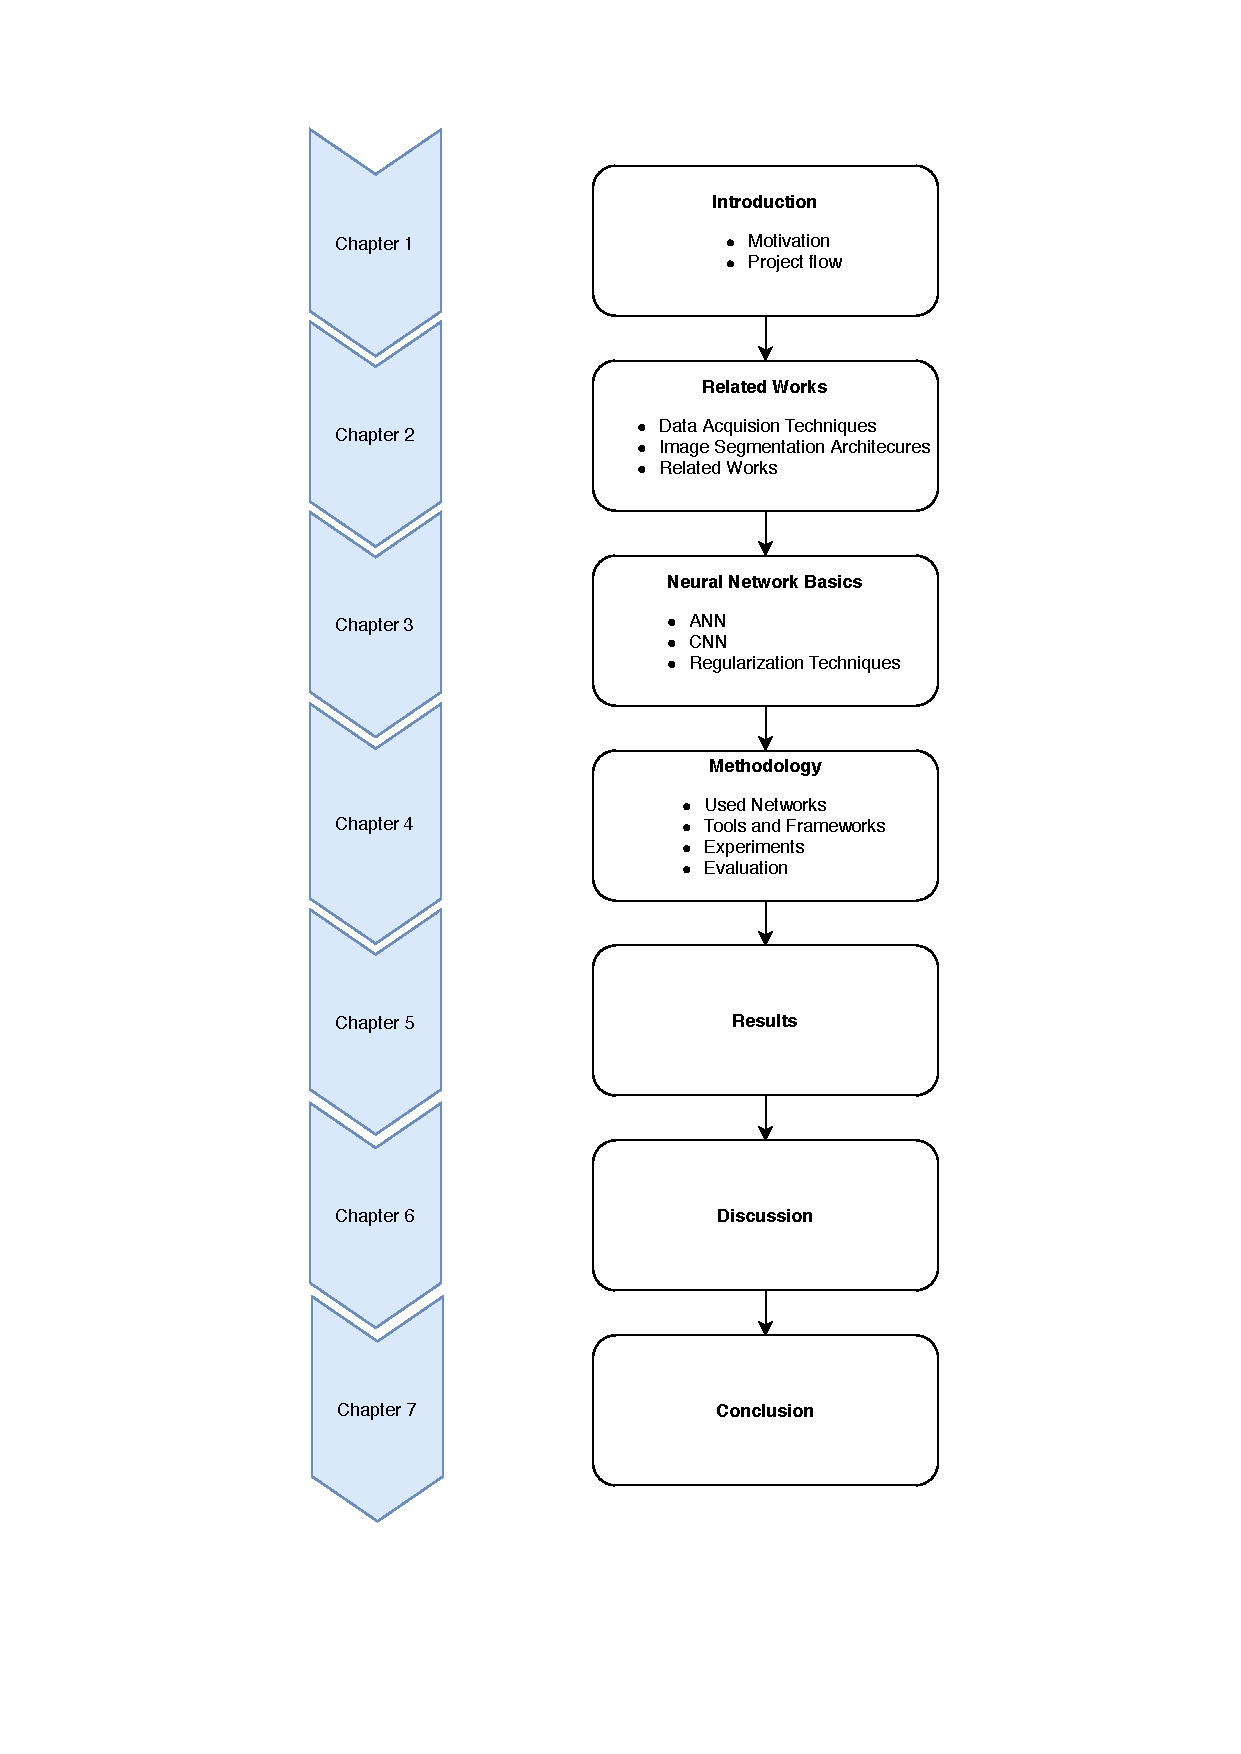
\includegraphics[width=1\columnwidth]{01-introduction/figures/project-flow.pdf}}
    \caption{ Thesis flow }
    \label{figure:project-flow}
\end{figure}

In this thesis, we provide a new application area of deep neural networks in skin lesion analysis.
We note that dermoscopic feature extraction is relatively a new problem in deep learning to address the detection and the classification of lesions.
The following section presents the medical imaging techniques, image segmentation architectures for automatic diagnosis of skin lesions from dermoscopic images and related studies of DNN for medicine.
The third section shows the basis of neural networks and convolutional neural networks.
Used neural network architectures, dataset, tools and deep learning frameworks are explained in fourth section
along with our corresponding formulation through computational parameters and the statistical evaluation.
Our detection results are given through statistical parameters in the fifth section.
Finally, the assessment of examined neural networks in skin lesion detection is concluded through the current state-of-the-art and prospective improvements.
The flow of the study in this thesis is summarized in Figure ~\ref{figure:project-flow}.

%
\chapter{Related Works}
\thispagestyle{empty}

    In this section, both common medical imaging techniques and dermatology imaging techniques are presented.
    Furthermore, skin lesion segmentation is detailed through commonly image segmentation architectures.
    Finally, related works are given to illustrate recent approaches in dermoscopic image analysis

    \section{Medical Imaging Techniques}

    Medical Image Segmentation aims to determine the location and shape of the body part or structure within a 2D or 3D image automatically or semi-automatically \cite{merjulah2019classification}.
    Medical images are created by many different modalities which will be examined below in detail.
    Wide modality range and the high variability of human anatomy is the major difference of medical image segmentation.
    Medical images are divided into several interests related with the problem definition to detect or segment the tumor or mass.
    Irregularities, blurred vision borders, low contrast between lesion and skin, air bubles are the some of various artifacts that makes segmentation medical imaging challenging \cite{guo2019neutrosophic}.

    Medical Imaging Techniques (MIT) are concerned to create medical images to be able to examine internal structures of body without opening up it \cite{kasban2015comparative}.
    In this section, common medical imaging techniques are being investigated.

    \subsection{Common Medical Imaging Techniques}

        \begin{figure}
    \centerline{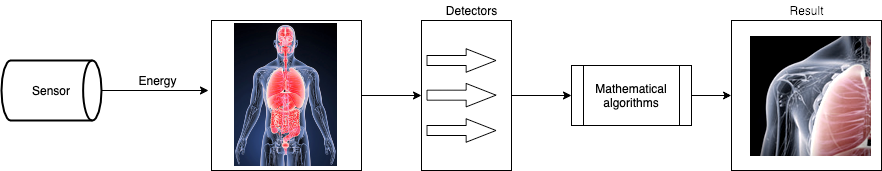
\includegraphics[width=1\columnwidth]{02-related-works/figures/medical-imaging-system-concept.png}}
    \caption{Medical Imaging Concept}
    \label{fig:medical-imaging-system-concept}
\end{figure}

        This section represent the review of widely-used medical imaging techniques namely X-ray Radiography, Magnetic Resonance Imaging, and Computed Tomography.

        \paragraph{X-ray Radiography} is an imaging technique that uses ionizing electromagnet radiation, such as X-ray which is a type of high-energy electromagnetic radiation \cite{kasban2015comparative}.
            As it can be seen at Figure~\ref{fig:sample-xray-images}, there is a trade-off between radiation level and image contrast which should be chosen carefully.
            X-ray passes through the body and is absorbed at different levels according to several factors such as the different tissue density.
            Mammography which deals with the scanning of breast tissue is one of the well-known application areas of X-ray Radiography.

            \begin{figure}
    \centerline{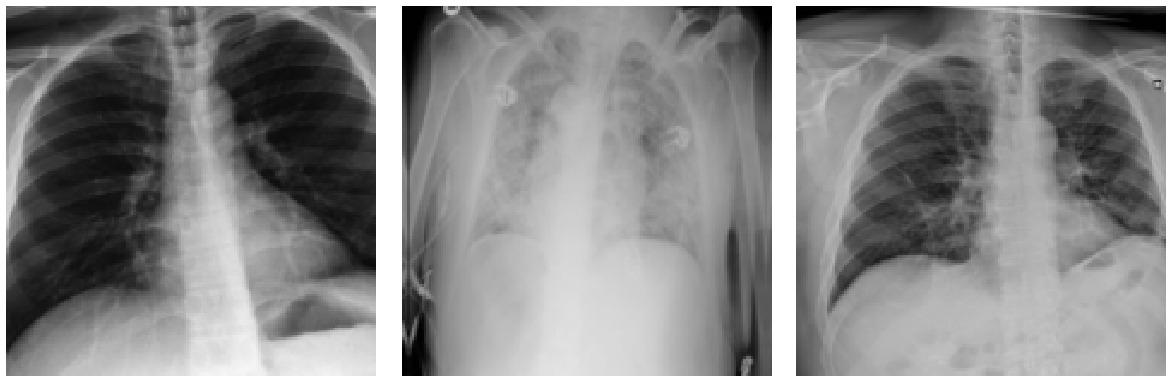
\includegraphics[width=1\columnwidth]{02-related-works/figures/sample-xray-images.png}}
    \caption{Sample X-ray Images \cite{ChestXRa12online}}
    \label{figure:sample-xray-images}
\end{figure}

        \paragraph{Magnetic Resonance Imaging (MRI)} is a commonly used imaging techniques for medical tasks
            which uses magnetic fields and frequencies in the radio wave spectrum to create images of body tissue \cite{mehmood2013prioritization}.
            Magnetic spin relaxation times and proton density changes can be used as distinctive in detecting abnormal tissues.
            MRI is based on visualizing these changes.
            MRI imaging can be enhanced by using a contrast solution, e.g. gadolinium, which will change the relaxation properties of some tissues under certain conditions.

            \begin{figure}
    \centerline{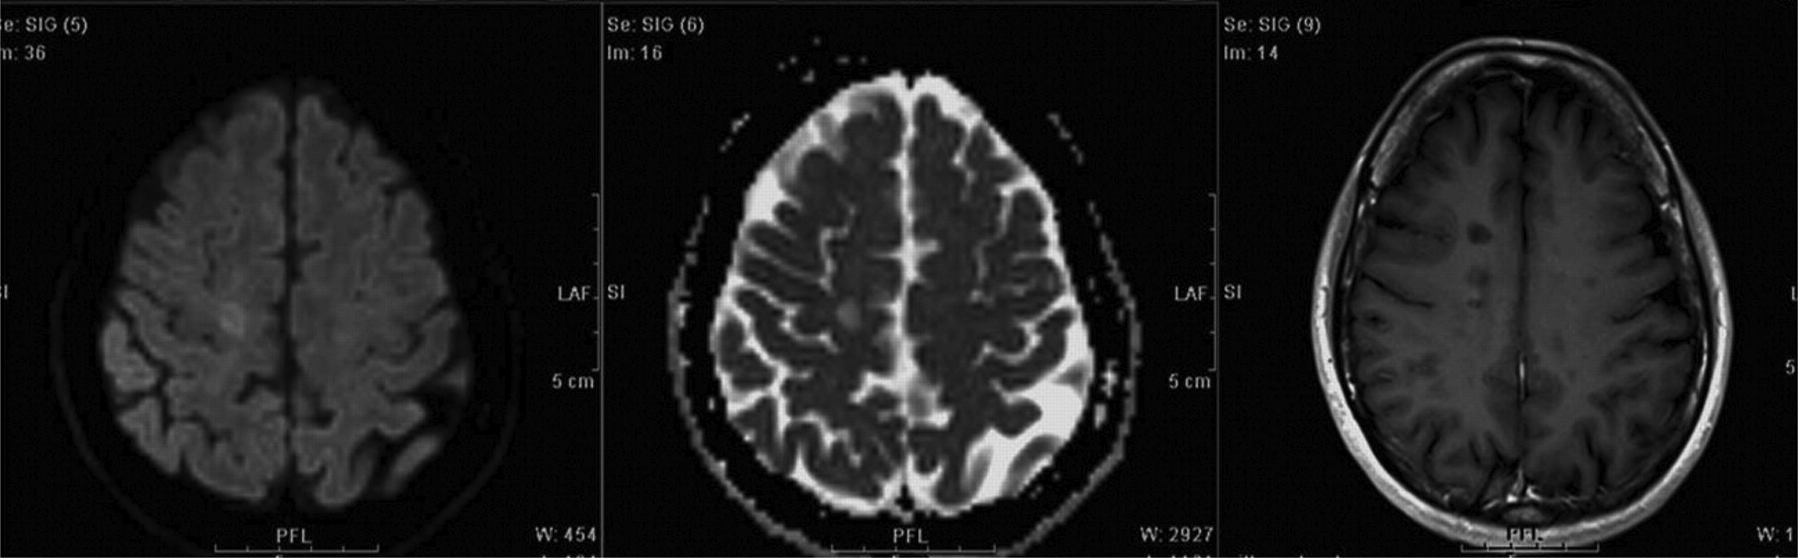
\includegraphics[width=1\columnwidth]{02-related-works/figures/sample-mri-images.png}}
    \caption{Sample MRI Images \cite{lovblad2010mr}}
    \label{figure:sample-mri-images}
\end{figure}

            Advantages of using MRI include painless, ionizing-free radiation, and high spatial resolution with operator independent usage.
            However, it may hard to use in people who cannot remain calm, and because of the relatively long scanning and post processing time, MRI does not offer real time results.
            An MRI sample is shown in Figure~\ref{fig:sample-mri-images}.

        \paragraph{Computed Tomography (CT)} is a computerized X-ray diagnostic imaging test which is supported with a cathode ray tube used to create detailed image of parts of the human body such as internal organs, blood vessels, bones and soft tissues \cite{Computed66online}.
            CT scanning is a common method in cancer diagnosis, as it is widely used to determine the size and location of a tumor.
            It is used to create not only for two dimensional (2D) images but also for three dimensional (3D) images using spiral CT which is basically reconstructing the collected volume data to provide 3D images.
            Figure~\ref{fig:sample-ct-images} shows some examples of generated CT images.

            \begin{figure}
    \centerline{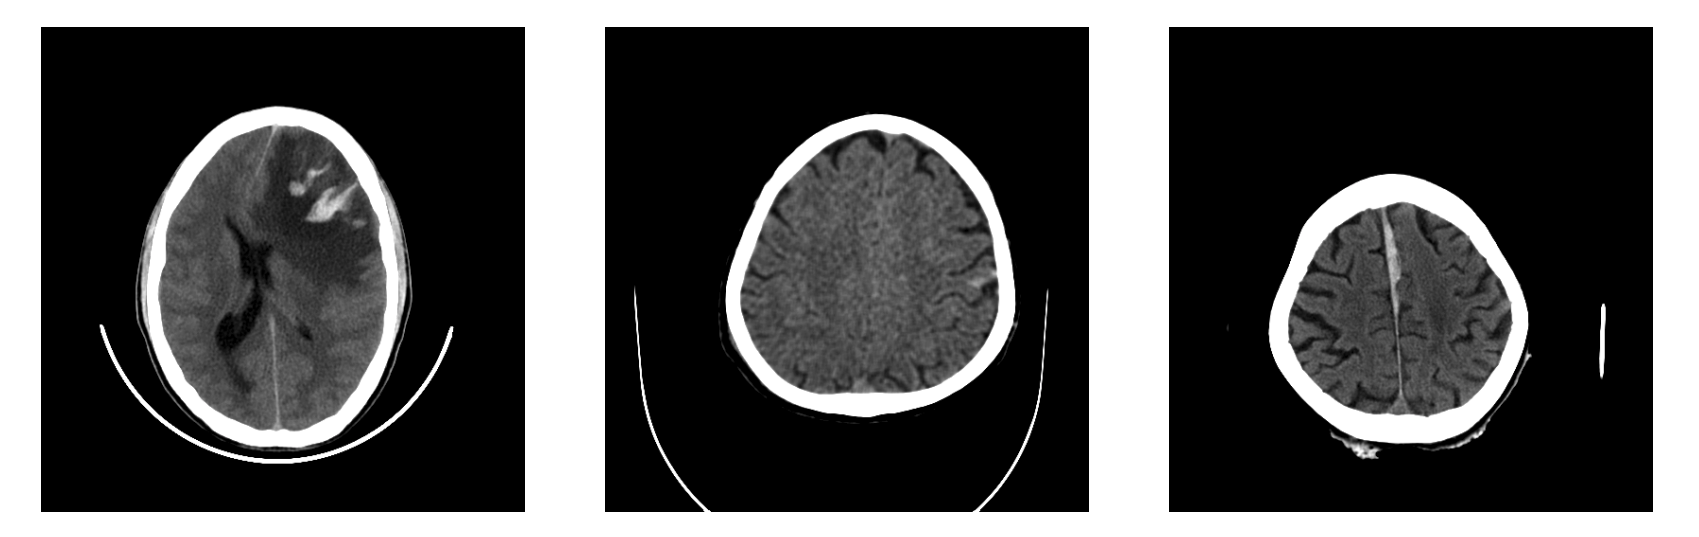
\includegraphics[width=1\columnwidth]{02-related-works/figures/sample-ct-images.png}}
    \caption{Sample CT Images \cite{chilamkurthy2018deep}}
    \label{fig:sample-ct-images}
\end{figure}

            Analyzing the parts of human body, diagnosing the abnormalities and traumas, observing the results of the cancer treatments are the common use cases of CTs.
            It comes with several benefits sucs as getting good spatial resolution, detecting issues quickly and painlessly.
            CTs, on the other hand, does not provide real time analysis and relatively useless results with the soft tissues with low contrast.

        %! Author = fatihergin
%! Date = 2020-05-03

\begin{table}[h]
\caption{Comparision of medical imaging techniques}
\centering
\begin{tabular}{c|cccc}
Imaging Techniques         & \begin{tabular}[c]{@{}c@{}}Spatial \\ resolution\end{tabular} & \begin{tabular}[c]{@{}c@{}}Good \\ contrast\end{tabular}          & Cost   & \begin{tabular}[c]{@{}c@{}}Real time \\ visualization\end{tabular} \\
\specialrule{2pt}{1pt}{1pt}
Ultrasonography            & 1mm                                                          & Soft tissues                                                      & Low    & Supported                                                           \\
X-ray                      & 1mm                                                          & \begin{tabular}[c]{@{}c@{}}Soft tissues \\ and fluid\end{tabular} & Medium & Unsupported                                                        \\
CT                         & 0.5mm                                                        & \begin{tabular}[c]{@{}c@{}}Hard and \\ soft tissues\end{tabular}  & High   & Unsupported                                                         \\
MRI                        & 0.5mm                                                        & \begin{tabular}[c]{@{}c@{}}Hard and \\ soft tissues\end{tabular}  & High   & Unsupported                                                         \\
\hline
\end{tabular}
\label{table:comparision-of-medical-imaging-techniques}
\end{table}

    \subsection{Skin Lesion Imaging Techniques}

        In this section, imaging techniques used in skin lesions are being investigated.

        \paragraph{Traditional Photography (TP)} is the well-known techniques which makes visualizing and monitoring the top layer of the lesion possible \cite{feit2004melanomas}.

        \paragraph{Dermoscopy Imaging Technique (DIT)}  is a real-time noninvasive diagnostic imaging technique
            which is more successful in distinguishing melanoma concentration than traditional photography \cite{aljanabi2019various}.

        \paragraph{Multispectral Imaging (MI)} provides information in both spectral and spatial domains.
            MI systems increase accuracy by calibrating image intensity,
            controlling exposure time automatically with the help of a multispectral camera that includes different optical filters selected by the problem definition.
            MI is used in medical imaging to support  detecting the lesions about 2mm \cite{aljanabi2019various}.
            Figure~\ref{fig:sample-multispectral-images} shows the images of a skin lesion taken by using different optical filters.

            \begin{figure}
    \centerline{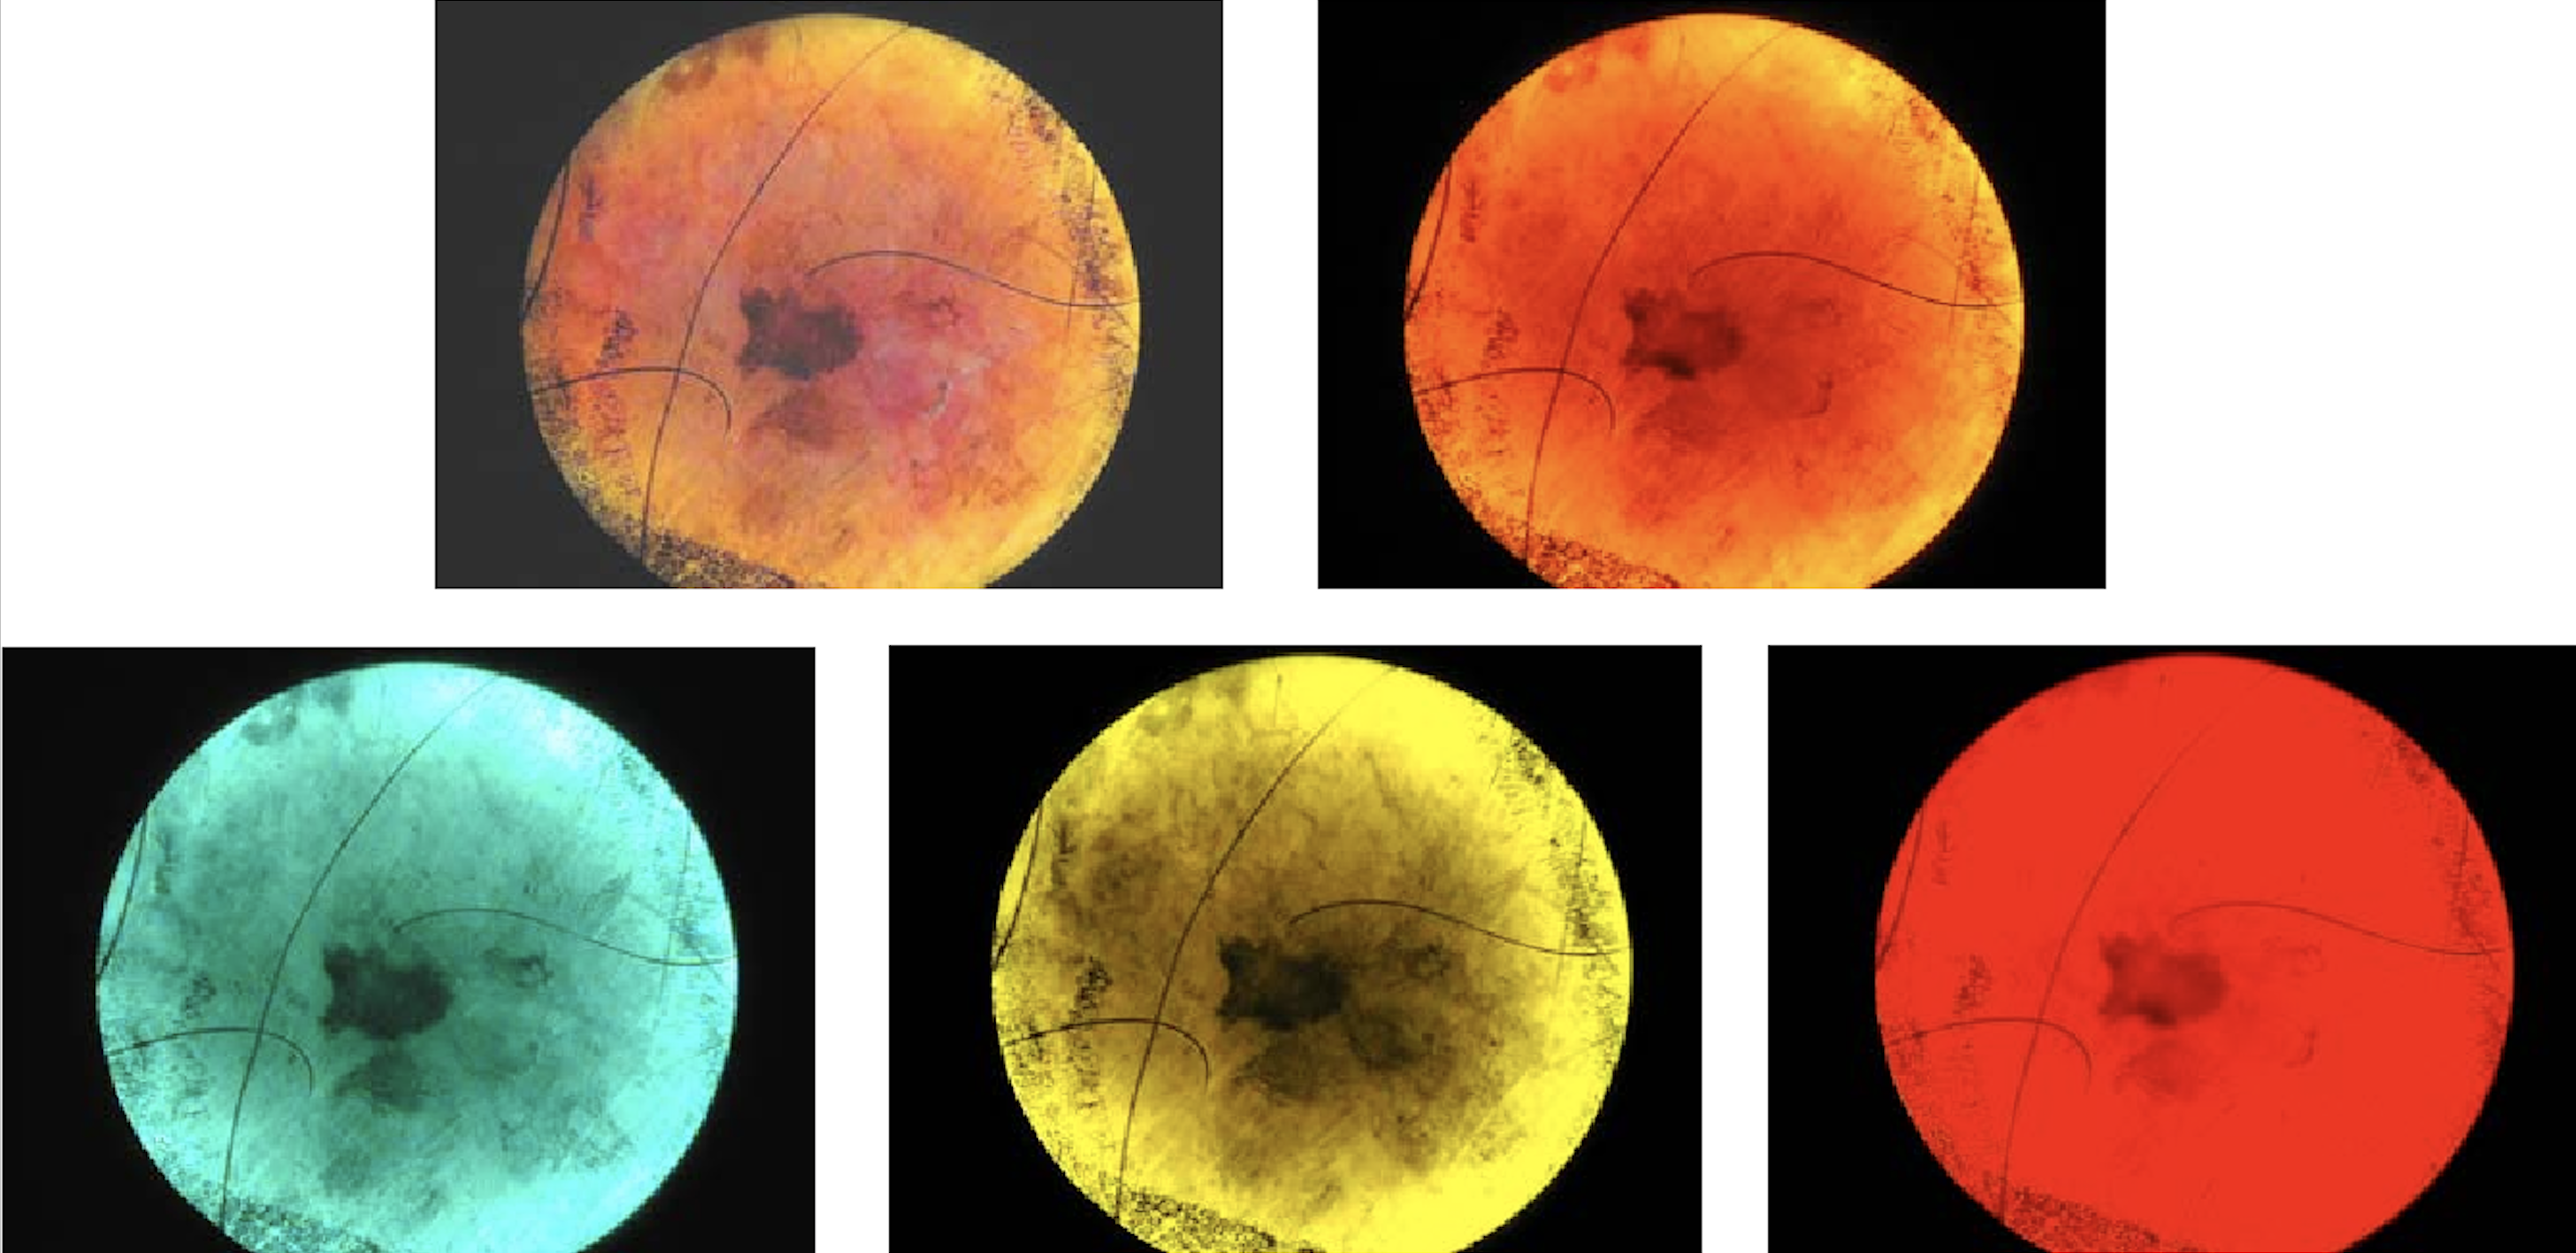
\includegraphics[width=1\columnwidth]{02-related-works/figures/sample-multispectral-images.png}}
    \caption{Sample Multispectral Images \cite{dhawan2009multispectral}}
    \label{figure:sample-multispectral-images}
\end{figure}

        \paragraph{Confocal Laser Scanning Microscopy (CLSM)} is an imaging technique that provides real-time details of skin morphology
            and provides images with the same resolution as traditional microscopes \cite{gerger2005diagnostic}.
            CLSMs are very sensitive for clinical applications but they are relatively expensive to use in there.
            From right to left clinical, dermoscopical, confocal images of a skin lesion is shown on Figure~\ref{fig:sample-clsm-images}.

            \begin{figure}
    \centerline{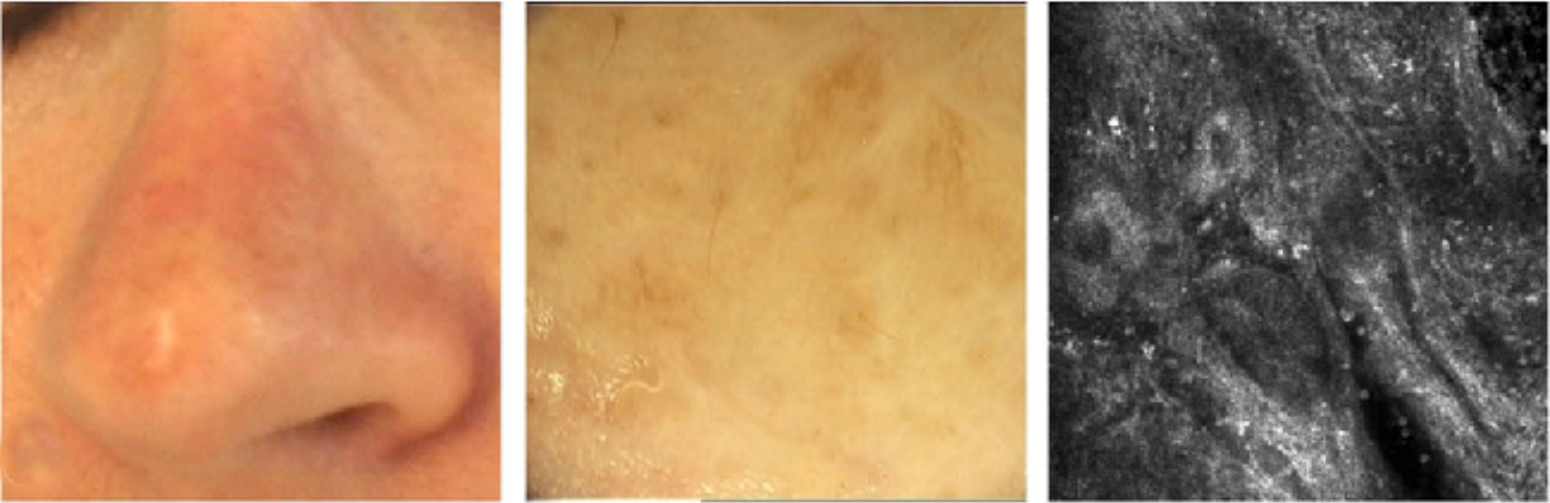
\includegraphics[width=1\columnwidth]{02-related-works/figures/sample-clsm-images.png}}
    \caption{From right to left clinical, dermoscopical, confocal images of a skin lesion \cite{ruini2016invisible}}
    \label{figure:sample-clsm-images}
\end{figure}

        \paragraph{Ultrasonography} which is also known as diagnostic sonography is another imaging technique that is used to create medical imaging to create internal body parts using high frequency broadband sound waves.
            Because different tissues behave differently under these sound waves,  the images generated using the waves reflected by tissue \cite{sahuquillo2013study}.
            Calculating the depth of skin cancer is the focused usage of Ultrasonography for this kind of projects.

            Ultrasonography offer painless real time visualization without ionized radiation in high resolution.
            But it is a time consuming and operator dependendent imaging technique.


    \section{Image Segmentation Architectures}

    Fully convolutional network (FCN) is a CNN variant which is a turning point for semantic segmentation literature \cite{long2015fully}.
    After that, many variants of CNN for segmentation has been developed.
    In this section, commonly used CNNs which are used for image segmentation starting from FCN are examined.

    \subsection{Fully Convolutional Network}

        Fully convolutional networks (FCNs) indicate that the convolutional neural networks are obtained by dismantling the fully connected layers from deep CNNs \cite{ulku2019survey}.
        FCNs are built on traditional classification networks such as VGG\cite{simonyan2014very}, AlexNet \cite{krizhevsky2012imagenet}, GoogLeNet\cite{szegedy2014going}, and ResNet\cite{he2016deep}.

        Convolutional layers are used instead of fully connected layers to produce outputs with the same size of inputs  instead of classification scores which are the outputs of CNNs.
        FCNs consist of two units encoding and decoding. Convolution and subsampling operations are performed in the encoding unit to encode the lower dimensional latent space.
        Deconvolution and upsampling are performed in the decoding unit which guarantee the obtaining the same size of output with the input.
        Because FCNs do not include fully connected layers, it is faster to inference an image if they are compared with the classical CNNs.

        Besides the including convolutional layers, skip architecture is one of the main reasons that makes FCNs faster over CNNs.
        Skip architectures help to prevent losing some information which can be lost because of the dropout or any other architectural decisions which may cause losing information.
        They provide flowing the summed or concatenated data between downsampling and upsamling blocks.
        Skip connections are also preserve the localised information which may lose on pooling layers with bypassing them.

    \subsection{SegNet}

        \citet{badrinarayanan2017segnet} proposed a FCN based network architecture, called SegNet, aiming to increase the accuracy of segmentation tasks.
        As it can be seen in Figure~\ref{figure:segnet-architecture}, the encoder network of the proposed method is consist of 13 convolutional layers of VGG16 network instead of the original fully connected layers of FCN.
        A pixel-wise classification layer is added to helps the upsampling on the lower resolution images in the decoder network.
        The upsampling part is the novel improvement of SegNet.

        \begin{figure}
    \centerline{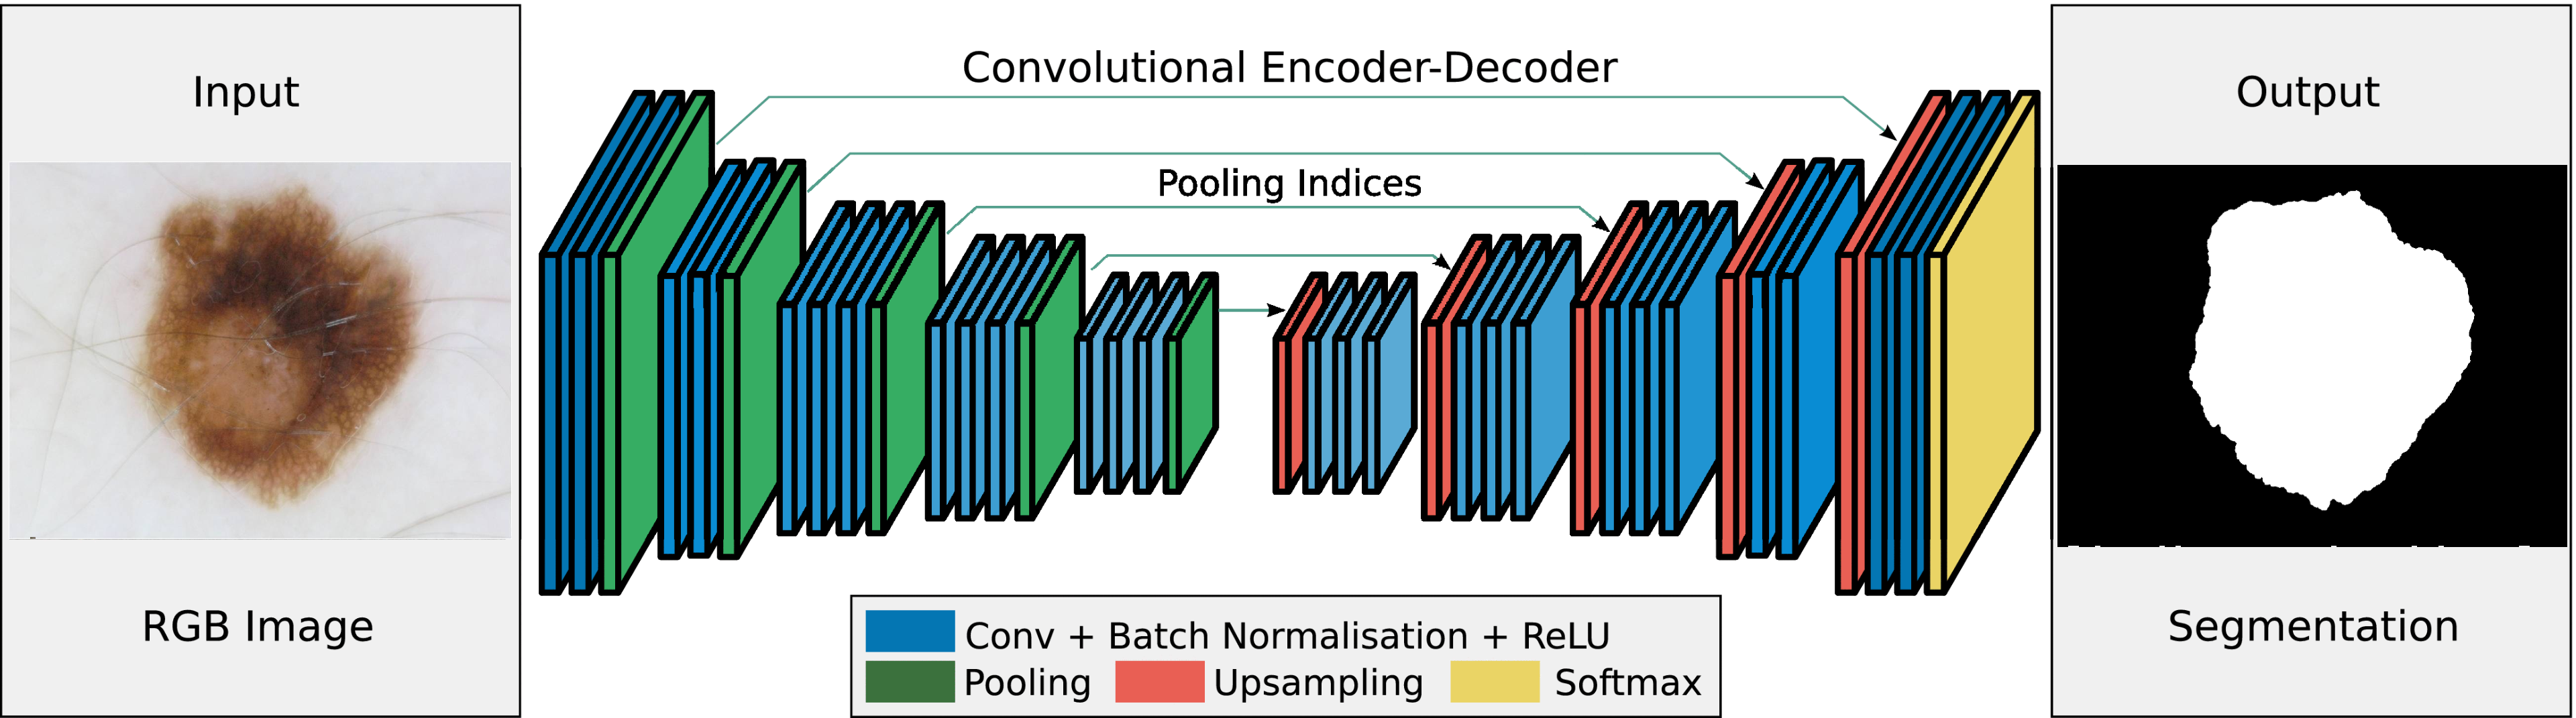
\includegraphics[width=1\columnwidth]{02-related-works/figures/segnet-architecture.png}}
    \caption{ SegNet architecture \cite{badrinarayanan2017segnet} }
    \label{figure:segnet-architecture}
\end{figure}

        Encoder is not fully connected in Segnet causes the train parameters to decrease by ~90\%.
        There is a corresponding decoder for every 13 encoders and they are responsible for upsampling of the feature map.

    \subsection{U-Net}\label{section:unet}

        \citet{ronneberger2015u} proposed a new CNN namely U-Net designed for medical imaging.
        Because medical image segmentation suffers from lack of large dataset, it is relatively hard to capture image context with localized lesions.
        U-Net aims to achieve competitive results even if the training data are relatively small.

        \begin{figure}
    \centerline{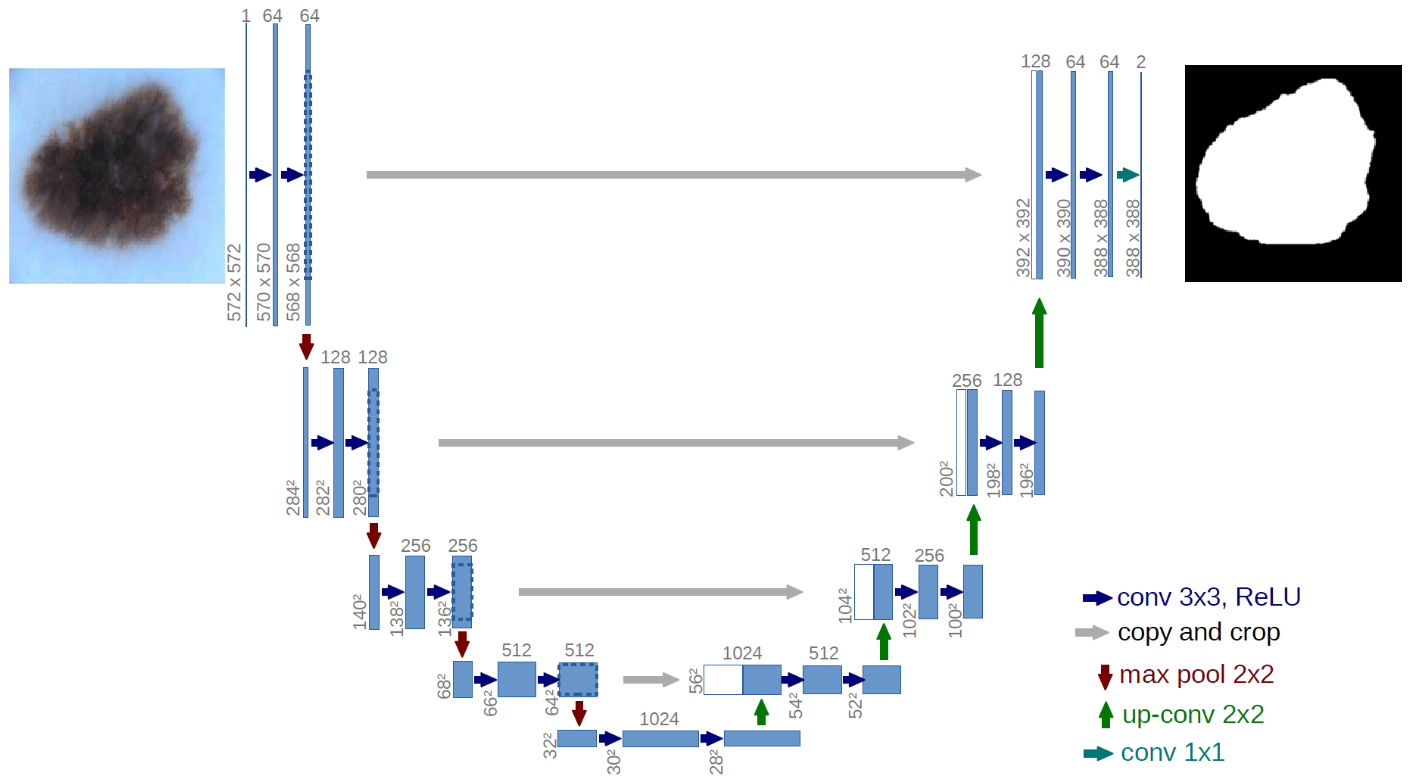
\includegraphics[width=1\columnwidth]{02-related-works/figures/u-net-architecture.png}}
    \caption{ U-Net architecture \cite{ronneberger2015u} }
    \label{fig:unet-architecture}
\end{figure}

        Classical feed-forward CNNs can learn many small information with details with the help of the fully connected layers because large datasets provide a number of parameters to train.
        On the contrary, large datasets oftenly are not exist or not accesible in medical imaging.
        Thus, if the neural network aims to accurate results with them, each image in dataset needs to be learnt deeply to extract the features.
        Up convolutions of the decoder unit which is a replacement of fully connected layers still have trainable parameters and this makes U-Net relatively more successful with smaller datasets by capturing context in detail.
        As it can be shown in Figure~\ref{figure:unet-architecture}, U-Nets are made up of contracting and expansive paths on the left and right respectively.

        The purpose of the contracting path is to increase resolutions and learn features  to capture context while the role of the expanding path is to aid in precise localization with a series of upsampling operations.
        The contracting path consist of two three-by-three convolutions followed by a ReLU and two-by-two max pooling layers.
        On the other side, up convolution layers exist to upsample the outputs.
        Skip connections help to prevent to lose the spatial context combining with upsampled outputs by transfering the low resolution features to expanding path.
        The authors used a large-weighted loss function to separate boundaries of background labels and touching segments which is a known problem of medical image segmentation.

    \subsection{Generative Adversarial Network}

        \citet{goodfellow2014generative} proposed a deep learning framework which is called generative adversarial network (GAN) consisting of two neural networks namely generator and discriminator.
        The proposed network can be considered as an autoencoder trying to produce a fake version of the real data.

        The generator which is the first part of the GANs, generates a sample and the discriminator interprets the sample as a real or fake.
        The ‘real’ means that whether the source of the data is training set. The flow can be seen in Figure~\ref{figure:gan-architecture}.

        \begin{figure}
    \centerline{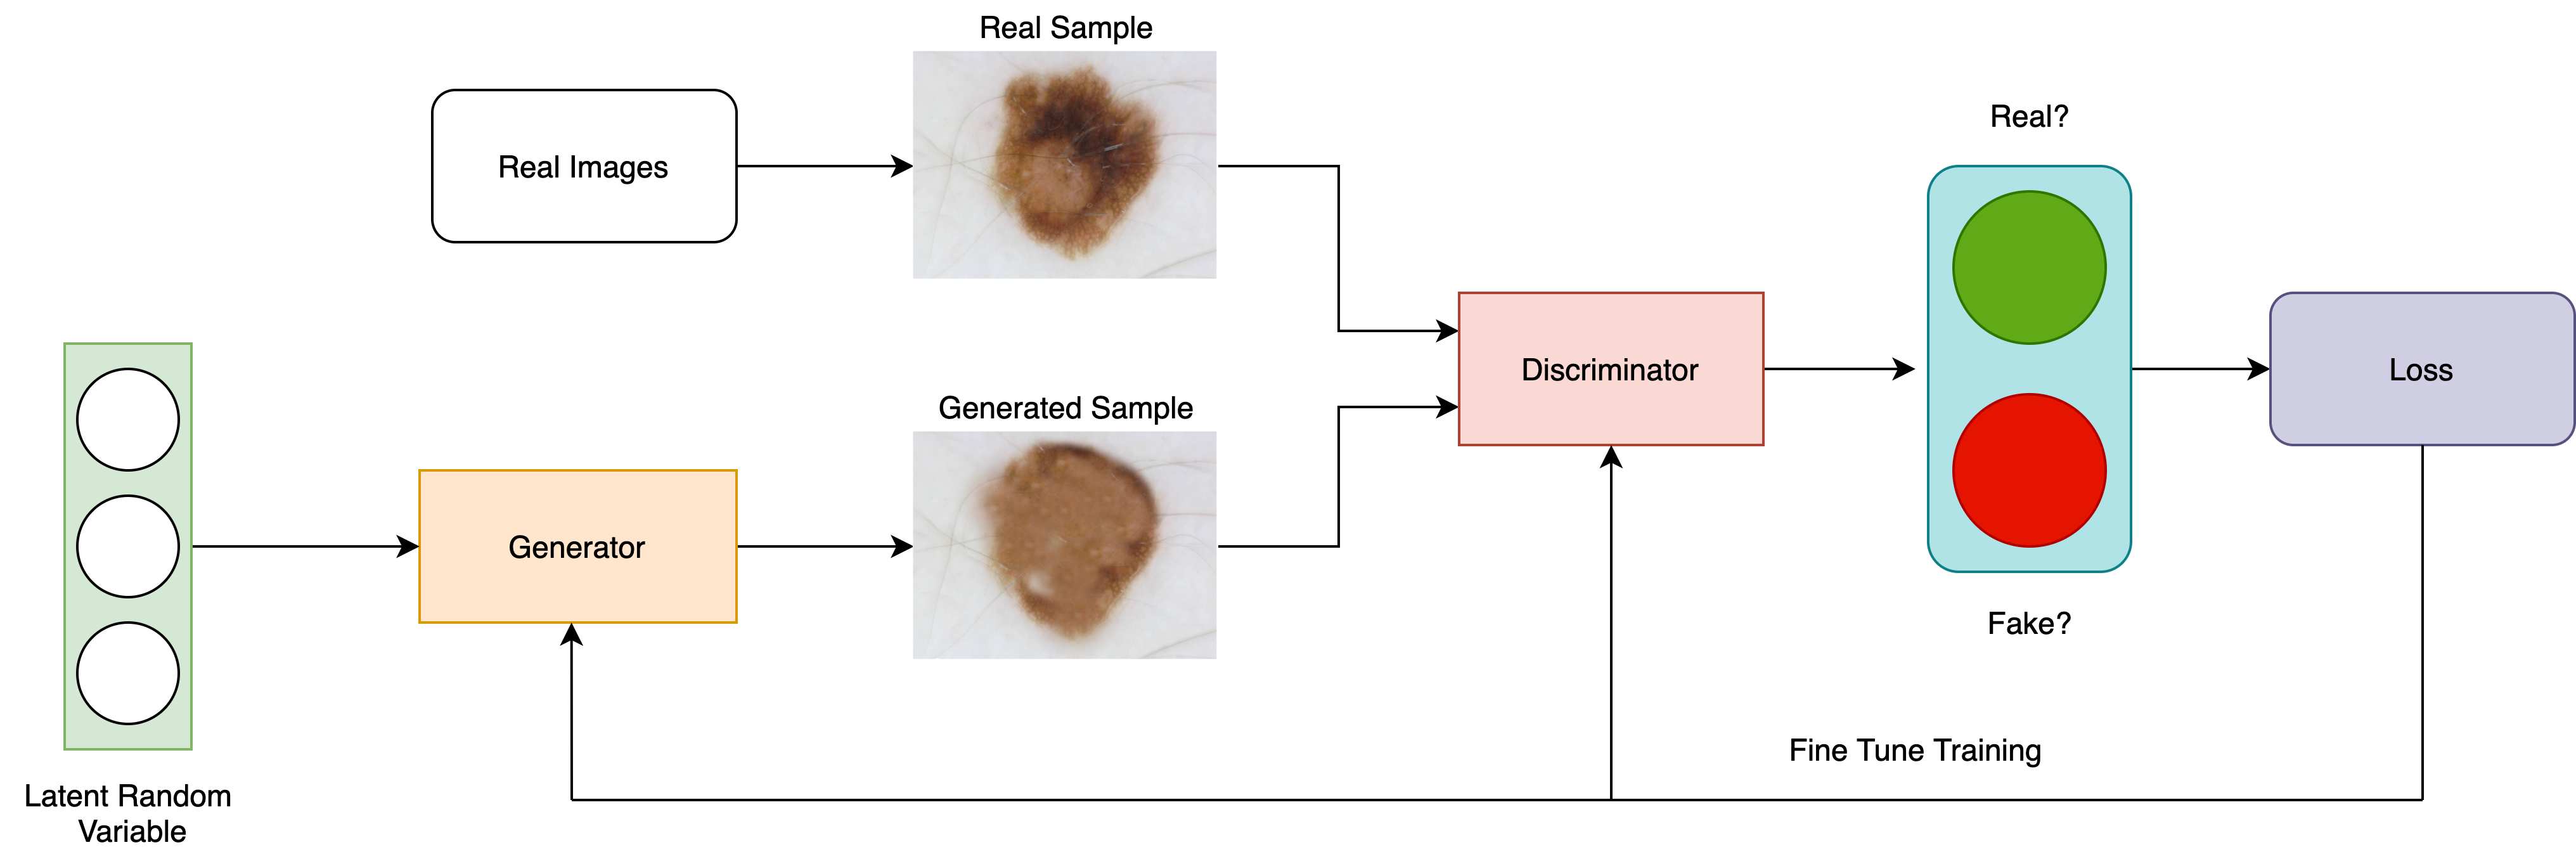
\includegraphics[width=1\columnwidth]{02-related-works/figures/gan-architecture.png}}
    \caption{ GAN architecture }
    \label{figure:gan-architecture}
\end{figure}

        It looks like a game where the generator tries to fool the discriminator with the samples it creates.
        The generator are update itself using the output of the discriminator on each iteration and gives better results.
        GANs have proved its success in many image analysis tasks, such as creating very realistic synthetic images \cite{shrivastava2017learning},
        domain adaption \cite{bousmalis2017unsupervised} and data completion \cite{yeh2017semantic}.
        Such successful applications of GANs to image processing tasks.


    \section{Related Works}

    Publication of AlexNet in 2012 have triggered a paradigm change in image segmentation, and then
    deep learning methods have provided prominent results and became the state-of-the-art in this area in recent years \cite{quang2017automatic}.
    In this section, the studies that propose deep architectures for skin lesion segmentation are discussed.
    Table~\ref{table:summary-of-related-skin-lesion-segmentation-surveys} shows the summary of the discussed surveys.

    \citet{long2015fully} proposed an FCN from the CNNs known to be successful in semantic segmentation.
    They adapted well-known classification networks such as AlexNet, VGG, GoogleLeNet to fully convolutional networks.
    Then, to create a successful segmentation, they combined semantic details from a deep layer
    and the appearance details from a shallow layer to define a new skip architecture.
    The proposed architecture achieved remarkable results compared to state-of-the-art models on PASCAL VOC.

    \citet{ronneberger2015u} built a new neural network aimed to be able to get accurate results with insufficient data by using them more effectively.
    U-Net, the proposed network, is based on classical FCNs and consist of two symmetric paths
    namely contracting and expanding which is responsible for capturing the context and enabling precise localization respectively.
    The new neural network proved its success with very few images by  winning the International Symposium on Biomedical Imaging (ISBI) 2015 Cell Tracking Challenge.
    In addition to being able to work with insufficient data, U-Net offers prominent results for training duration with images with relatively higher resolutions such as 512x512.
    In the following years, new studies showed that the proposed U-shaped network is more successful than C-Means Clustering in ISBI 2017 challenge dataset \cite{lin2017skin}.

    \citet{yuan2017automatic} introduced an improved version of FCN model using Jaccard distance as loss function.
    The aim of this network is increasing segmentation accuracy with
    solving common dermoscopic image problems such as imbalanced skin and lesion pixels, the existence of various artifacts, and irregular lesion borders.
    The proposed network achieved better results than the other state-of-the-art networks in ISBI 2016 challenge and PH2 databases.

    \citet{yuan2017automatic2} presented a new skin lesion segmentation framework base on Fully Convolutional Deconvolutional Neural Networks (CDNN).
    Their main focus is to improve network architecture rather than pre and post processings.
    Rectified Linear Unit (ReLU) is used as the activation of each layer in the network except to output layer.
    Internal covariate shift is reduced by adding batch normalization to the output of CD layers.
    The proposed CDNN model won the ISBI 2017 challenge.

    \citet{yuan2017improving} improved their other skin lesion segmentation architectures by using smaller kernels to optimize the discriminant capacity of their newly proposed neural network.
    The improved version of the previous work is evaluated on the ISBI 2017 challenge dataset and placed among the top 21 in the ranking.

    \citet{bi2017dermoscopic} proposed a multistage FCN to increase segmentation accuracy of classical FCNs.
    In this network, first stage FCN focused on learning localization information and coarse appearance,
    whereas second stage FCN focused on subtle characteristics of the lesion boundaries.
    A parallel integration method is also introduced to combine the results of the first and second stage FCNs.
    \citet{yu2018melanoma} presented a novel deep neural network architecture  consisting of two stages called segmentation and classification.
    The network combines a deep learning method with a local descriptor encoding strategy for dermoscopy image recognition.
    A pretrained large image dataset is used to extract deep representations of a rescaled image.
    After that, extracted descriptors are aggregated and encoded with a Fisher Vector to get global features.
    At the end, the global features are used to classify images with the help of a support vector machine.
    The proposed network is a fully convolutional residual network (FCRN) and took second place in the segmentation category of the ISBI 2016 challenge.

    \citet{al2018skin} developed a framework for skin lesion segmentation via full resolution convolutional networks (FrCN).
    This method eliminated subsampling layers and learned the full resolution features directly.
    It is tested with ISBI 2017 challenge and PH2 datasets and has achieved better results against the well-known state-of-the-art segmentation networks such as U-Net, SegNet and FCN.

    \citet{li2018dense} introduced a new dense deconvolutional network (DDN) for skin lesion segmentation.
    The proposed network is based on residual learning. It consist of three main parts namely dense convolutional layer, hierarchical supervision (HS), and chained residual pooling (CRP).
    Dimensions of the input and output images remain unchanged in DDLs.
    CRP helps to capture contextual background features while HS is responsible for improving the prediction mask.
    They tested the network with the ISBI 2017 dataset and it achieved 86.6\% Dice coefficient indices.

    \citet{xue2018adversarial} proposed an Adversarial Neural Network (GAN), called SeGAN, based deep neural network aimed to increase accuracy of medical image segmentation.
    Classical GANs are not as good as expected in providing gradient feedback to the network, because their output is single which may not represent pixel level details of images.
    Segmentation label maps are created with the help of newly created FCN based segmentor network with a new activation function.
    Another significant improvement in the proposed network is multi-scale L1 loss function aimed to extract both local and global features which represent the relations between pixels.

    \citet{peng2019segmentation} introduced a new adversarial network based segmentation architecture consisting of a CNN based discrimination and a U-Net based segmentation networks.
    This utilized generative adversarial network is evaluated on the ISBI 2016 challenge dataset and achieved 97.0\% Accuracy rate.

    \citet{tu2019segmentation} proposed an adversarial network based deep learning framework focused on solving the imbalanced lesion-background problem.
    The segmentation block of the proposed network is an encoder-decoder network with Dense-Residual block. Deep supervision is utilized with a multi-scale loss function.
    The network is evaluated on the ISBI 2017 challenge dataset and gained better segmentation results than the other state-of-the-art methods participating in that challenge.

    \citet{tschandl2019domain} introduced a new FCN where pretrained ImageNet weights are being used to feed the network on ResNet34 layers which are reused as encoding layers.
    The evaluation results showed that using pretrained weights improved the segmentation score on the ISBI 2017 challenge dataset.

    \citet{ninh2019skin} proposed a SegNet architecure based FCN framework
    which aimed to decrease the number of upsampling and downsampling layers of classical SegNet architecture to reduce the learned parameters.
    The proposed network is evaluated on the ISBI 2017 challenge dataset and gained sufficient results in terms of Jaccard Index and Dice coefficient.

    \citet{mirikharaji2019learning} proposed a deep CNN framework focused on segmenting skin lesions.
    The main focus of the proposed network was the use of two different annotation set consisting of reliable and unreliable annotations.
    The reliable annotations are marked by experts and showed reliable segmentation results. This reweighting is done by a newly deployed meta-learning approach.
    The proposed network shows that using different levels of annotation noise on weighting affects the segmentation results and model robustness positively.

    \citet{sarker2019mobilegan} proposed a lightweight GAN framework, called MobileGAN, aiming to reduce the number of training parameters while keeping the segmentation accuracy high.
    They combined the channel attention module with the 1D non-bottleneck factorization networks for the generator part of the GAN.
    MobileGAN is trained with ISIC 2018 training dataset and was evaluated with ISBI 2017 challenge dataset.
    Compared to state-of-the-art models such as FCN, U-Net, or SegNet, the results showed that the proposed network had fewer parameters, about 2.3 million, and achieved considerable scores.

    \citet{lei2020skin} proposed a GAN framework aiming to increase skin lesion segmentation accuracy and won the first part of ISBI 2017 challenge.
    The segmentation part of the proposed GAN was construct with a skip connection and dense convolution U-Net while the discrimination part was consist of a dual discriminator module.
    One of the discriminators was responsible for increasing the detection of boundaries while the other one was responsible for learning the contextual informations.

    \citet{zafar2020skin} proposed an automated neural network architecture aimed to segment skin lesion accurately.
    Res-Unet, the proposed network, is a combination of two well-known neural networks in image segmentation namely U-Net and ResNet.
    The other major improvement in this network is using image inpainting for hair removal.
    It was evaluated on the ISBI 2017 challenge and PH2 datasets and gained Jaccard Index of 77.2\% and 85.4\%  respectively.

    \citet{xie2020mutual} introduced a CNN variant, called MB-DCNN, which consisted of three sub CNNs namely coarse segmentation network,
    mask guided segmentation network, and enhanced segmentation network respectively.
    The first network was responsible for creating coarse masks which had been used on the next network to classify the lesions.
    The third network was a segmentation network fedded from the second classification network.
    There were learning transfer between networks to increase the segmentation accuracy.
    MB-DCNN was tested with the ISBI 2017challenge and PH2 datasets and it achieved Jaccard index of 80.4\% and 89.4\%.

    %! Author = fatihergin
%! Date = 2020-05-03

\begin{longtable}{c|cccc}
\caption{Summary of related skin lesion segmentation surveys} \\
Publication                       & Architecture & Title                                                                                                                                                 & Highlights \\
\specialrule{2pt}{1pt}{1pt}
\citet{long2015fully}             & FCN          & \begin{multilinetable}Fully convolutional networks for semantic segmentation\end{multilinetable}                                                      & \begin{multilinetable}The first FCN implementation for semantic segmentation\end{multilinetable}   \\
\specialrule{0.5pt}{1pt}{1pt}
\citet{ronneberger2015u}          & U-Net        & \begin{multilinetable}U-net: Convolutional networks for biomedical image segmentation\end{multilinetable}                                             & \begin{multilinetable}A new architecture focused on medical image segmentation\end{multilinetable}   \\
\specialrule{0.5pt}{1pt}{1pt}
\citet{yuan2017automatic}         & FCN          & \begin{multilinetable}Automatic skin lesion segmentation using deep fully convolutional networks with jaccard distance\end{multilinetable}            & \begin{multilinetable}Jaccard distance bases loss function\end{multilinetable}   \\
\specialrule{0.5pt}{1pt}{1pt}
\citet{yuan2017automatic2}        & CDNN         & \begin{multilinetable}Automatic skin lesion segmentation with fully convolutional-deconvolutional networks\end{multilinetable}                        & \begin{multilinetable}Adding batch normalization to the output of CD layers\end{multilinetable}   \\
\specialrule{0.5pt}{1pt}{1pt}
\citet{yuan2017improving}         & CDNN         & \begin{multilinetable}Improving dermoscopic image segmentation with enhanced convolutional-deconvolutional networks\end{multilinetable}               & \begin{multilinetable}Discriminant capacity is optimized with smaller kernels\end{multilinetable}   \\
\specialrule{0.5pt}{1pt}{1pt}
\citet{bi2017dermoscopic}         & FCN          & \begin{multilinetable}Dermoscopic image segmentation via multistage fully convolutional networks\end{multilinetable}                                  & \begin{multilinetable}Multistage FCN with localized responsibilities\end{multilinetable}   \\
\specialrule{0.5pt}{1pt}{1pt}
\citet{yu2018melanoma}            & FCRN         & \begin{multilinetable}Melanoma recognition in dermoscopy images via aggregated deep convolutional features\end{multilinetable}                        & \begin{multilinetable}A pretrained dataset is used to extract deep representations of images\end{multilinetable}   \\
\specialrule{0.5pt}{1pt}{1pt}
\citet{al2018skin}                & FrCN         & \begin{multilinetable}Skin lesion segmentation in dermoscopy images via deep full resolution convolutional networks\end{multilinetable}               & \begin{multilinetable}Eliminates subsampling layers and learns the full resolution features directly\end{multilinetable}   \\
\specialrule{0.5pt}{1pt}{1pt}
\citet{li2018dense}               & DDN          & \begin{multilinetable}Dense deconvolutional network for skin lesion segmentation\end{multilinetable}                                                  & \begin{multilinetable}Residual learning based 3 layered network\end{multilinetable}   \\
\specialrule{0.5pt}{1pt}{1pt}
\citet{xue2018adversarial}        & SeGAN        & \begin{multilinetable}Adversarial learning with multi-scale loss for skin lesion segmentation\end{multilinetable}                                     & \begin{multilinetable}GAN based network with multi-scale loss function\end{multilinetable}   \\
\specialrule{0.5pt}{1pt}{1pt}
\citet{peng2019segmentation}      & GAN          & \begin{multilinetable}Segmentation of dermoscopy image using adversarial networks\end{multilinetable}                                                 & \begin{multilinetable}Consist of A CNN based discrimination and a U-Net based segmentation networks\end{multilinetable}   \\
\specialrule{0.5pt}{1pt}{1pt}
\citet{tu2019segmentation}        & GAN          & \begin{multilinetable}Segmentation of Lesion in Dermoscopy Images Using Dense-Residual Network with Adversarial Learning\end{multilinetable}          & \begin{multilinetable}Dense-Residual Network based segmentation block\end{multilinetable}   \\
\specialrule{0.5pt}{1pt}{1pt}
\citet{tschandl2019domain}        & FCN          & \begin{multilinetable}Domain-specific classification-pretrained fully convolutional network encoders for skin lesion segmentation\end{multilinetable} & \begin{multilinetable}Encoding layers are fed with pretrained weight\end{multilinetable}   \\
\specialrule{0.5pt}{1pt}{1pt}
\citet{ninh2019skin}              & SegNet       & \begin{multilinetable}Skin Lesion Segmentation Based on Modification of SegNet Neural Networks\end{multilinetable}                                    & \begin{multilinetable}Reduces the training parameters while keeps the accuracy\end{multilinetable}   \\
\specialrule{0.5pt}{1pt}{1pt}
\citet{mirikharaji2019learning}   & CNN          & \begin{multilinetable}Learning to segment skin lesions from noisy annotations\end{multilinetable}                                                     & \begin{multilinetable}Reliable and unreliable annotation sets are used together\end{multilinetable}   \\
\specialrule{0.5pt}{1pt}{1pt}
\citet{sarker2019mobilegan}       & MobileGAN    & \begin{multilinetable}MobileGAN: Skin Lesion Segmentation Using a Lightweight GAN\end{multilinetable}                                                 & \begin{multilinetable}Reduces the training parameters while keeps the accuracy\end{multilinetable}   \\
\specialrule{0.5pt}{1pt}{1pt}
\citet{lei2020skin}               & GAN          & \begin{multilinetable}Skin Lesion Segmentation via Generative Adversarial Networks with Dual Discriminators\end{multilinetable}                       & \begin{multilinetable}Dual discriminator module are used for discrimination block\end{multilinetable}   \\
\specialrule{0.5pt}{1pt}{1pt}
\citet{zafar2020skin}             & Res-Unet     & \begin{multilinetable}Skin Lesion Segmentation from Dermoscopic Images Using Convolutional Neural Network\end{multilinetable}                         & \begin{multilinetable}Combination of U-Net and ResNet\end{multilinetable}   \\
\specialrule{0.5pt}{1pt}{1pt}
\citet{xie2020mutual}             & MB-DCNN      & \begin{multilinetable}A Mutual Bootstrapping Model for Automated Skin Lesion Segmentation and Classification\end{multilinetable}                      & \begin{multilinetable}Consists of three sub CNNs with different responsibilities\end{multilinetable}   \\
\hline
\end{longtable}
\label{table:summary-of-related-skin-lesion-segmentation-surveys}




%
\chapter{Neural Networks in Tumor Detection}

    In this section, firstly Artificial Neural Networks (ANNs), and then Convolutional Neural Networks (CNNs) are examined
    with the commonly used regularization techniques in the orientation of tumor detection.

    %! Author = fatihergin
%! Date = 2020-05-03

\section{Artificial Neural Networks}

    ANNs are a category of supervised machine learning algorithms whose design has been inspired by the neurophysiological workings of the human brain \cite{hill1994artificial}.
    These networks consist of several layers mainly first layer, last layer and middle layer(s).
    The first layer is known as the input layer, middle layer which is called as hidden layer and the last layer is the output layer where each layer has several artificial neurons.
    An example of ANN with a single hidden layer can be seen at Figure~\ref{figure:simple-ann}.
    The most common layer organization is the fully connected layer, where each neuron is fully paired with adjacent neurons.

    An ANN transform the inputs into outputs using the activation function, bias and weights.
    To explain, the sum of inputs is multiplied by weights; the deviation is added and the result is passed through the activation function which is selected by purpose.
    Deciding whether the neuron is active is determined by the activation function.

    \begin{figure}
    \centerline{\scalebox{0.65}{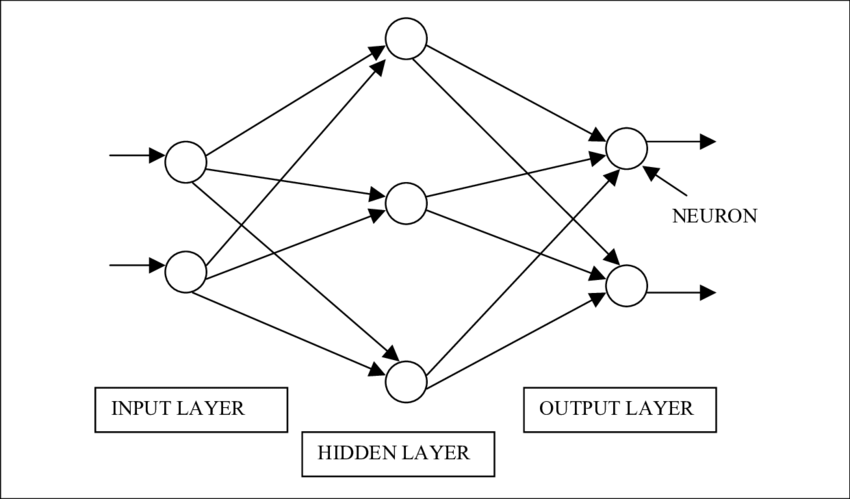
\includegraphics{03-neural-networks-in-tumor-detection/figures/simple-ann.png}}}
    \caption{A sample ANN model}
    \label{figure:simple-ann}
\end{figure}

    During the training, training samples are sent one by one through the network.
    The output value is calculated for each sample sent.
    Output values are compared to the target with the help of a loss function to minimize the error rate.
    At the backpropagation step, the network is updated by propagating errors backwards through the network \cite{lecun1988theoretical}.

    \subsection{Weight Update}

        Gradient descent is used to minimize the loss function of the neural network.
        The first-order derivative of the loss function, namely gradient is computed at the current point and it is used to increase the slope in the opposite direction by moving in by the value of self.
        These two steps are applied to the weights in each cycle.
        Batch gradient descent (BGD), stochastic gradient descent (SGD), and mini-batch gradient descent are some of the commonly used weight update methods.
        In SGD, the training samples are randomly shuffled, to put it another way, the weights are updated after each training sample \cite{bottou2010large}.
        On the other hand, all the training samples are used at weight update in batch gradient descent.
        SGD requires more calculations than batch gradient descent and it is more sensitive than the other.
        Because SGD is suitable for larger datasets and batch gradient descent is for the smaller datasets, mini-batch gradient descent which is a combination of SGD and batch gradient descent is developed.
        It use a batch of a limited number of samples to update the weights.

    \subsection{Activation Functions}

        An activation function is used to decide whether an artificial neuron should be activated by calculating the weighted sum of its input.
        To explain, it basically decides whether the information that the neurons receive is relevant, and ignores it if not.
        The activation functions can be basically divided into 2 groups as linear and non-linear activation functions.
        Because linear functions have constant derivatives, there is no relation between the derivative of the linear function and the input value of x.
        Therefore, the output of functions will not be limited across any range.

        \begin{figure}
    \centerline{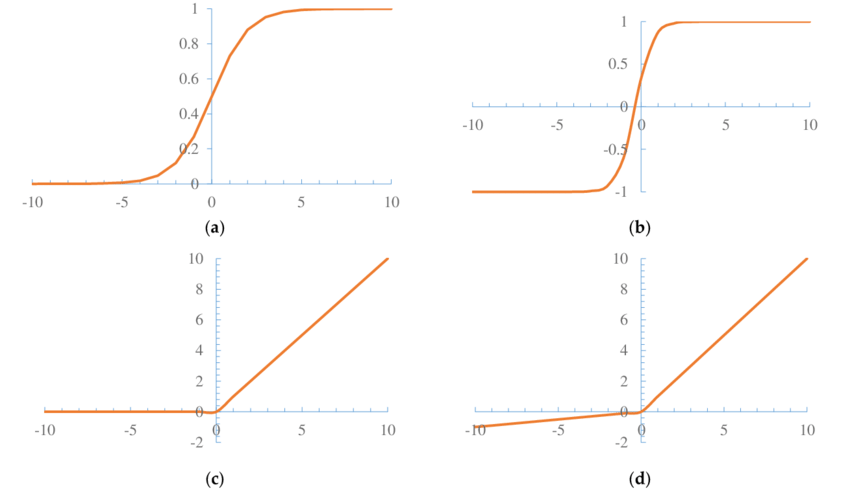
\includegraphics[width=1\columnwidth]{03-neural-networks-in-tumor-detection/figures/nonlinear-activation-functions.png}}
    \caption{Nonlinear activation functions \textbf{(a)} Sigmoid, \textbf{(b)} Tanh, \textbf{(c)} ReLU, and \textbf{(d)} Leaky ReLU \cite{yang2018modified}}
    \label{figure:nonlinear-activation-functions}
\end{figure}

        The non-linear activation functions which are preferred over the linear activation functions can be seen in Figure ~\ref{figure:nonlinear-activation-functions}.
        It helps to the model to generalize or adapt data. They are basically grouped by their curves and ranges.
        Commonly used activation functions such as Softmax, Sigmoid, Tanh, ReLU, Leaky ReLU and PReLU are examined in this section.

        \begin{itemize}

            \item \textbf{Sigmoid} functions are smooth and continuously differentiable which means the slope of the Sigmoids can be found for any two points.
                    The Sigmoids are monotonic but their derivatives are not.
                    In Sigmoids, the Y values tend to respond very less to changes in X as it can be seen in Equation \eqref{equation:sigmoid}.
                    It means that small changes in the X values will cause larger changes in the Y values in this range.
                    So the purpose of this function is to try to keep the Y values to the extremes.
                    This is helpful when classifying the values into a particular class.
                    If they are compared to linear functions, the outputs are always stay in a fixed range (0,1) unlike the linear functions whose outputs can be in the range of infinity.
                    It is clearly understood that the Sigmoid function produces positive values for all the points and it is not symmetric around the origin.

                    \begin{equation}
                        h_ \theta (x) =  \frac{\mathrm{1} }{\mathrm{1} + e^- \theta^Tx } \label{equation:sigmoid} \\
                    \end{equation}

            \item \textbf{Softmax} is a Sigmoid function derivative which gives remarkable results in multi variant image classification.

                    \begin{equation}
                        y_i(z_i) = \frac{e^{z_i}}{ \sum\nolimits_{k=1}^{k}{e^{z_k}} } \label{equation:softmax} \\
                    \end{equation}

            \item \textbf{Tanh} function is an activation function which is a scaled version of the Sigmoid function.
                    The difference between the Sigmoid and the Tanh is that the Tanh is symmetric over the origin whereas the Sigmoid is not symmetric, so the range of the Tanh is between -1 and 1.
                    Continuity and differantiability of the Tanh is similiar to the Sigmoid, it is continuous and differentiable.

                    \begin{equation}
                        tanh(x) = \frac{2}{(1+e^(-2x)) -1} \label{equation:tanh} \\
                    \end{equation}

                    It is preferred to Softmax if there are no more than two classes in a classification problem.
                    The advantage is that the negative inputs will be mapped strongly negative and the zero inputs will be mapped near zero in the Tanh graph.

            \item \textbf{Rectified Linear Unit (ReLU)} is an activation function which is non-linear and the most widely used activation function while designing neural networks today.

                    \begin{equation}
                          f(x) = x^+ = \max(0, x) \label{equation:relu} \\
                    \end{equation}

                    The non-linearity makes backpropagate the errors and have multiple layers of neurons being activated by ReLU function easy.
                    ReLU does not activate the all neurons at once
                    As it can be seen in Equation \eqref{equation:relu}, the neuron does not activated if the input is not positive.
                    This may cause the dead neurons problem which is the main problem of ReLU.
                    In this activation function, only a few neurons are activated at a time. This makes the network sparse means efficient and easy for computation.

            \item \textbf{Leaky ReLU} function is an improved version of the ReLU function.
                    The gradient which is \emph{0} for \emph{x < 0} in ReLU make the neurons die for activations in that region.
                    Leaky ReLU is focused on solving the dead neurons problem.
                    The function is defined as a small linear component of \emph{x}.

                    \begin{equation}
                         f(x) = \begin{cases} x &
                            \text{if } x > 0, \\
                            0.01x & \text{otherwise}.
                         \end{cases}\\
                    \end{equation}

            \item \textbf{PReLU} which is also known as Parameterised ReLU is very similar to the Leaky ReLU.

                    \begin{equation}
                         f(x) = \begin{cases}
                            x & \text{if } x > 0, \\
                            a x & \text{otherwise}.
                        \end{cases}
                    \end{equation}

                    In this context, \emph{a} is a trainable parameter which its values is learnt the network for faster and more optimum convergence.
                    PReLU is preferred when Leaky ReLU fails to passing the relevant information to the next layer with solving the dead neurons problem.

        \end{itemize}

    \subsection{Loss Functions}

        Loss function which is also called cost function evaluates the penalty between the ground truth label and the prediction during the training process to detect how well neural network models the dataset.
        The output of the loss function is inversely proportional to the success of the model, meanly higher numbers in the output are the sign of the unsuccessful model.
        Loss function is used the error which is calculated during backpropagation to update the weights in the negative direction of its derivative.

        In this section, some of the commonly used loss functions for image segmentation such as weighted cross entropy, balanced cross entropy, and Dice loss are examined.

        \begin{itemize}

            \item \textbf{Weighted Cross Entropy (WCE)} weights the classes based on the fraction of the respective class in the total dataset as it can be seen in Equation \eqref{equation:wce-loss} which is the definition of WCE for prediction \emph{p} and label $\hat{p}$.
                    Thus, a class with a low fraction of the pixels in the dataset will get a high weighting. This is particularly interesting when the dataset contains unbalanced classes.

                    \begin{equation}
                        \text{WCE}\left(p, \hat{p}\right) = -\left(\beta p \log\left(\hat{p}\right) + (1-p) \log\left(1 - \hat{p}\right)\right) \label{equation:wce-loss} \\
                    \end{equation}

                    $\beta \emph{> 1}$ should be setted to reduce the false negative rates while $\beta \emph{< 1}$ should be setted to reduce the false positive rates.

            \item \textbf{Balanced Cross Entropy (BCE)} another variant of cross entropy which differs from WCE is that weighting the negative examples also.

                    \begin{equation}
                        \text{BCE}\left(p, \hat{p}\right) = -\left(\beta p \log\left(\hat{p}\right) + (1 - \beta)(1-p) \log\left(1 - \hat{p}\right)\right) \label{equation:bce-loss} \\
                    \end{equation}

            \item \textbf{Dice Loss}\\

                    The values of Dice ranges from zero to one, and high value means high similarity between the segmentations.
                    For two overlapping regions, the Dice is defined as two times the intersection over the union.
                    Dice loss is defined in Equation \eqref{equation:dice-loss} for prediction \emph{p} and label $\hat{p}$.

                    \begin{equation}
                        \text{DL}\left(p, \hat{p}\right) = 1 - \frac{2\sum p_{h,w}\hat{p}_{h,w}}{\sum p_{h,w} + \sum \hat{p}_{h,w}} \label{equation:dice-loss} \\
                    \end{equation}

        \end{itemize}



    \section{Convolutional Neural Networks}

    A convolutional neural network (also known as CNN) is a deep neural network inspired in the behavior of biological systems through artificial neurons with learnable weights and biases for image recognition tasks.
    D.H Hubel and T.N Wiesel discovered that the visual cortex consists of receptive fields that detect light in overlapping subregions.
    It is the entry point of modeling CNNs \cite{hubel1968receptive}.
    Every neuron responds to stimuli in a restricted region, as in visual cortex of the human brain, and that the overlapping regions of the neurons together cover the entire visual area.

    \begin{figure}
    \centerline{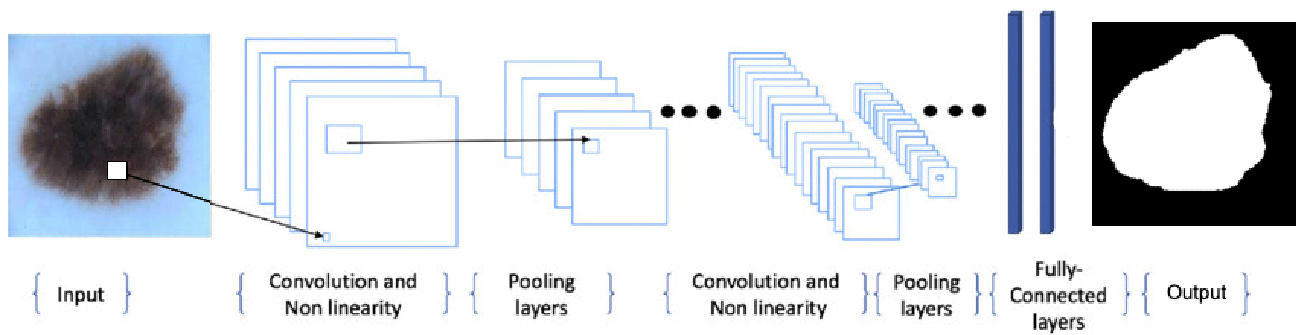
\includegraphics[width=1\columnwidth]{03-neural-networks-in-tumor-detection/figures/cnn-architecture-image-classification.png}}
    \caption{A CNN architecture for skin lesion classification}
    \label{figure:sample-cnn-architecture-skin-lesion-classification}
\end{figure}

    A CNN mainly consists of different types of layers as it can be seen in Figure~\ref{figure:sample-cnn-architecture-skin-lesion-classification} including input, convolutional, non-linearity, pooling, and fully connected layers.

    \begin{itemize}

        \item \textbf{Input layer} contains input images as a matrix of the raw pixel values.

        \item \textbf{Convolutional layer} is used to extract features of the input data.
            Each neuron has a local receptive field which means it is not fully connected, but connected to some section of the input to provide abstractions of small sections of the input data.
            Convolution layers calculate a dot product between the receptive field and the filter by performing convolution.
            The result of this convolution is a single integer which will be used as the input of the next layer.

            The filter is slided over the next receptive fields of the input image repeatedly until there is no unconvolved receptive field left.

        \item \textbf{Non-linearity layer} consists of an activation function, which applies an elementwise activation by thresholding at zero, creates and activation map with taking the output of the convolutional layer in CNNs.

        \item \textbf{Pooling layer} applies a spatial downsampling along the output volume.
            Pooling layers are commonly used to reduce the computational requirements of the neural networks progressively and minimize the overfitting.

        \item \textbf{Fully connected layer} mainly computes the class scores based on the training dataset.
            They connect the neurons in layers to each other.
            The last fully connected layer classifies the generated features with the help of an activation function.

    \end{itemize}




    \section{Regularization Techniques}

    \subsection{Data Augmentation}

        Data augmentation is artificially boosting the diversity and number of training examples by performing random transformations to existing images to create a set of new variants without altering the meaning of the data.
        Flipping, rotating, adding noise are the some of the commonly used data augmentation techniques.

        Data augmentation is used to prevent overfitting and especially useful when the training dataset is relatively small.
        While some augmentation increases the robustness of the algorithm, irrelevant transformations might make the task hard to learn, and adding new data to the training set will increase the model complexity and reqiured time to build the model.

    \subsection{Dropout}

        Overfitting is a common problem which is not limited only deep neural networks but includes the different disciplines such as several supervised and unsupervised methods in machine learning.
        Neural networks can be used to create relation between their input and output to predict the newly added input with acceptible result.
        It can be said that there is an overfitting if the results are not good for the unknown test data but good for the training data.

        Feeding the neural network with more training data is the simplest way which can be tried to prevent overfitting.
        This may effective if the newly added training data bring about new features which may increase the representativeness of the model. On the other hand, more training data will require more training time because it increase the model complexity.
        Bootstrap aggregating is another method which increase the network success \cite{breiman1996bagging}.
        This method classify different subsets of the training data, and fit a model based on these subsets.

        \citet{srivastava2014dropout} said that feature vectors should be combined instead of a single feature detector in order to describe meaningful features.
        They found out that  individual feature detectors start to detect helpful features afte dropping units from the neural network randomly.

        \begin{figure}
    \centerline{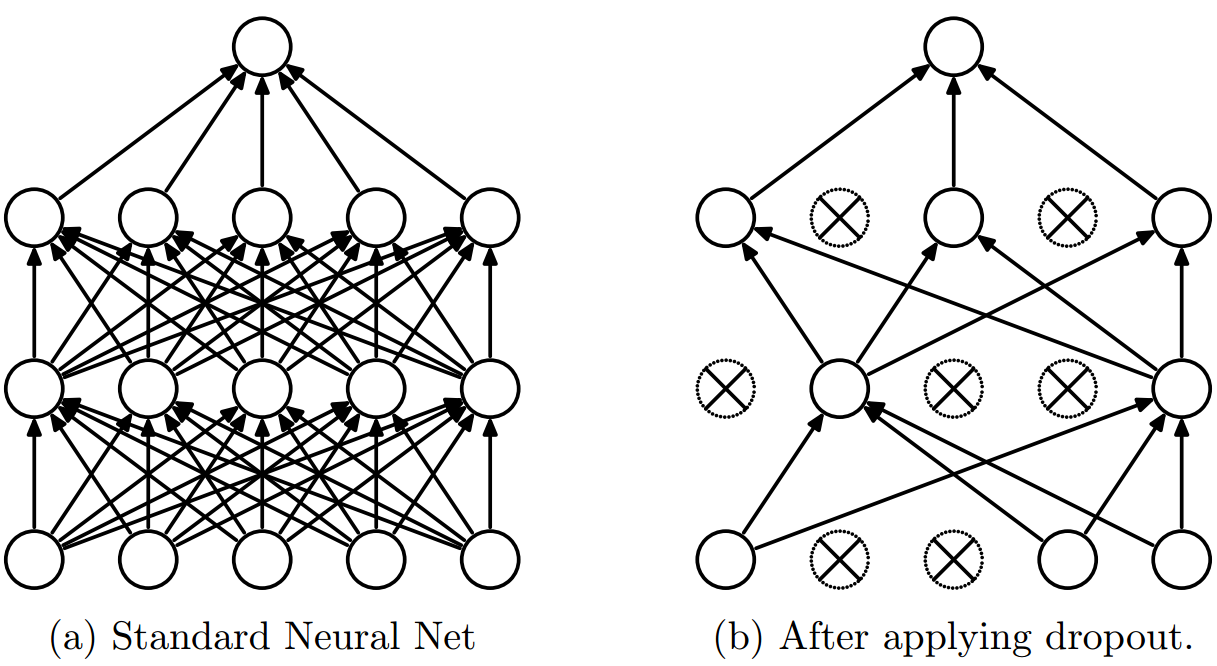
\includegraphics[width=1\columnwidth]{03-neural-networks-in-tumor-detection/figures/dropout.png}}
    \caption{ Dropout neural network model }
    \label{fig:dropout}
\end{figure}

        Dropout is a method of improvement aims to increase the performance of a neural network by reducing the overfitting \cite{srivastava2014dropout}.
        It's not only for CNNs but also all neural networks. At each training step, a new subset is excluded to improve the network's ability to generalize.
        The amount of exclusion is regulated by the dropout rate.
        Figure~\ref{fig:dropout} shows a regular neural network (a) and a thinned network by applying dropout (b).

    \subsection{Weight Decay}

        Weight decay is another technique used to prevent overfitting by adding a regularization term such as L1 or L2 to the loss function.
        L1 regularization is the sum of the absolute value of the weights and produces sparse weight matrices while L2 regularization is the sum of the squares of all the feature weights and make the calculation more computationally efficient.

        $$L_2\text{ regularization term} = ||\boldsymbol w||_2^2 = {w_1^2 + w_2^2 + ... + w_n^2}$$

        In L2 regularization, model complexity is dramatically affected by the outlier weights.

    \subsection{Early Stopping}

        Early stopping is a technique to reduce overfitting using the some part of the training data as a validation set.
        Training process does not include this data.
        If the error of the validation set reaches a certain amount, training is stopped at the training phase.
        It can be said that there is an overfitting exists in the current neural network for the training data.

        A significant point of eary stopping is selection of the validation set.
        It should represent the all data. It can be understood how well the model is generalizing beyond the training data.



%
\chapter{Methodology}

\section{Dataset}\label{sec:dataset}

The first part of ISBI Challenge 2017 \cite{codella2018skin} - Skin Lesion Analysis Towards Melanoma Detection: Lesion Segmentation dataset is used in this project.
This dataset has train, validation and test data separately. The training dataset consist of 2000 dermoscopic .jpg images and the related masks with .png format.
The dataset include various type of lesions namely malignant melanoma, nevus and seborrhoeic keratosis.
Sample images is given with corresponding masks in Figure ~\ref{fig:sample-images-from-dataset}.

\begin{figure}
    \centerline{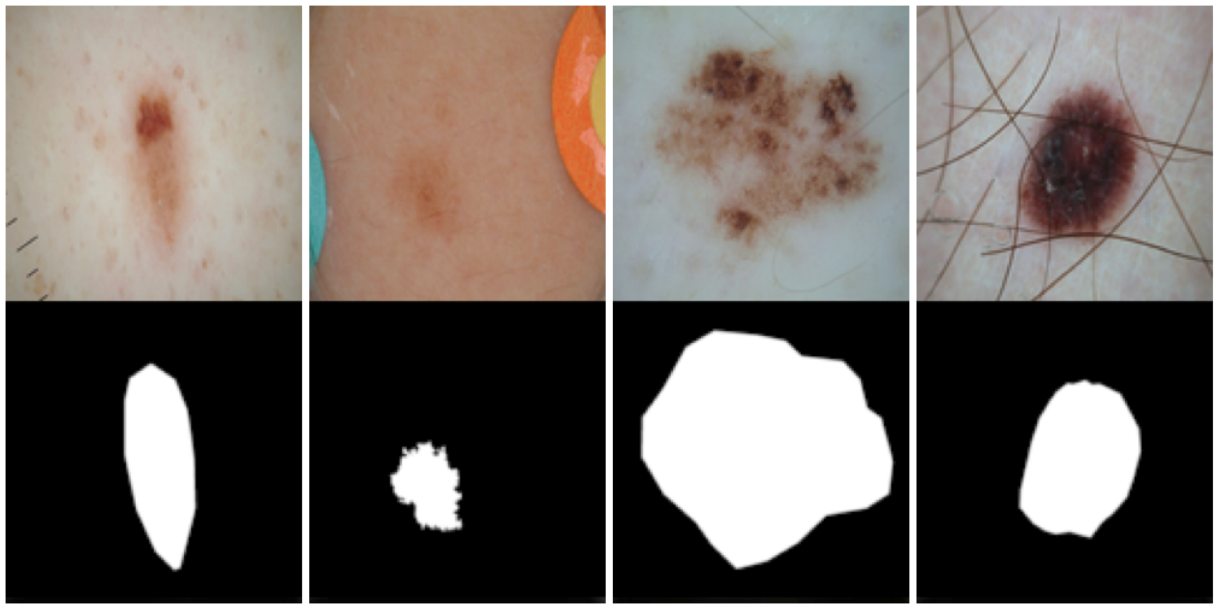
\includegraphics[width=1\columnwidth]{04-methodology/figures/sample-images-from-dataset.png}}
    \caption{Sample images from dataset. First row is original images, second row is corresponding masks}
    \label{figure:sample-images-from-dataset}
\end{figure}

There are also validation and test datasets which contain 150 and 600 images respectively.
The results are based on several common image similarity metrics which are given related section.

\begin{figure}
    \centerline{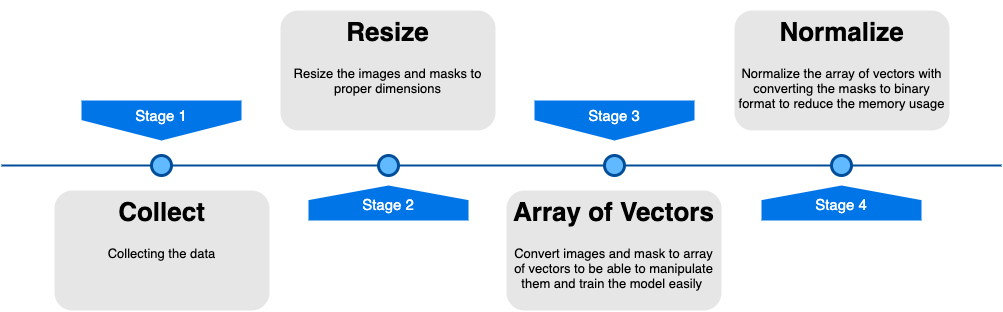
\includegraphics[width=1\columnwidth]{04-methodology/figures/data-preparation-process.png}}
    \caption{Data preparation process}
    \label{figure:data-preparation-process}
\end{figure}

The images are of various dimensions and the all used neural networks can't handle relatively big images because of their different internal architectures and memory constraints.
We also had to resize all images into same dimension to reduce the memory consumption and increase the accuracy as a preprocessing stage.
As it can be stated at Figure~\ref{fig:data-preparation-process}, arrays of mask files converted to uint8 to reduce the size of the masks.

    
\section{Networks}\label{sec:networks}

    In this section, the architectures used in this project are examined.

    \subsection{MultiResUNet}\label{sec:multiresunet}

        As discussed in Section~\ref{sec:unet}, U-Net is a state-of-the-art neural network in medical imaging, but it has some drawbacks in certain conditions.
        Starting from this point, \citet{ibtehaz2020multiresunet} proposed a new U-Net variant, MultiResUNet including several modifications examined below.

        \begin{figure}
    \centerline{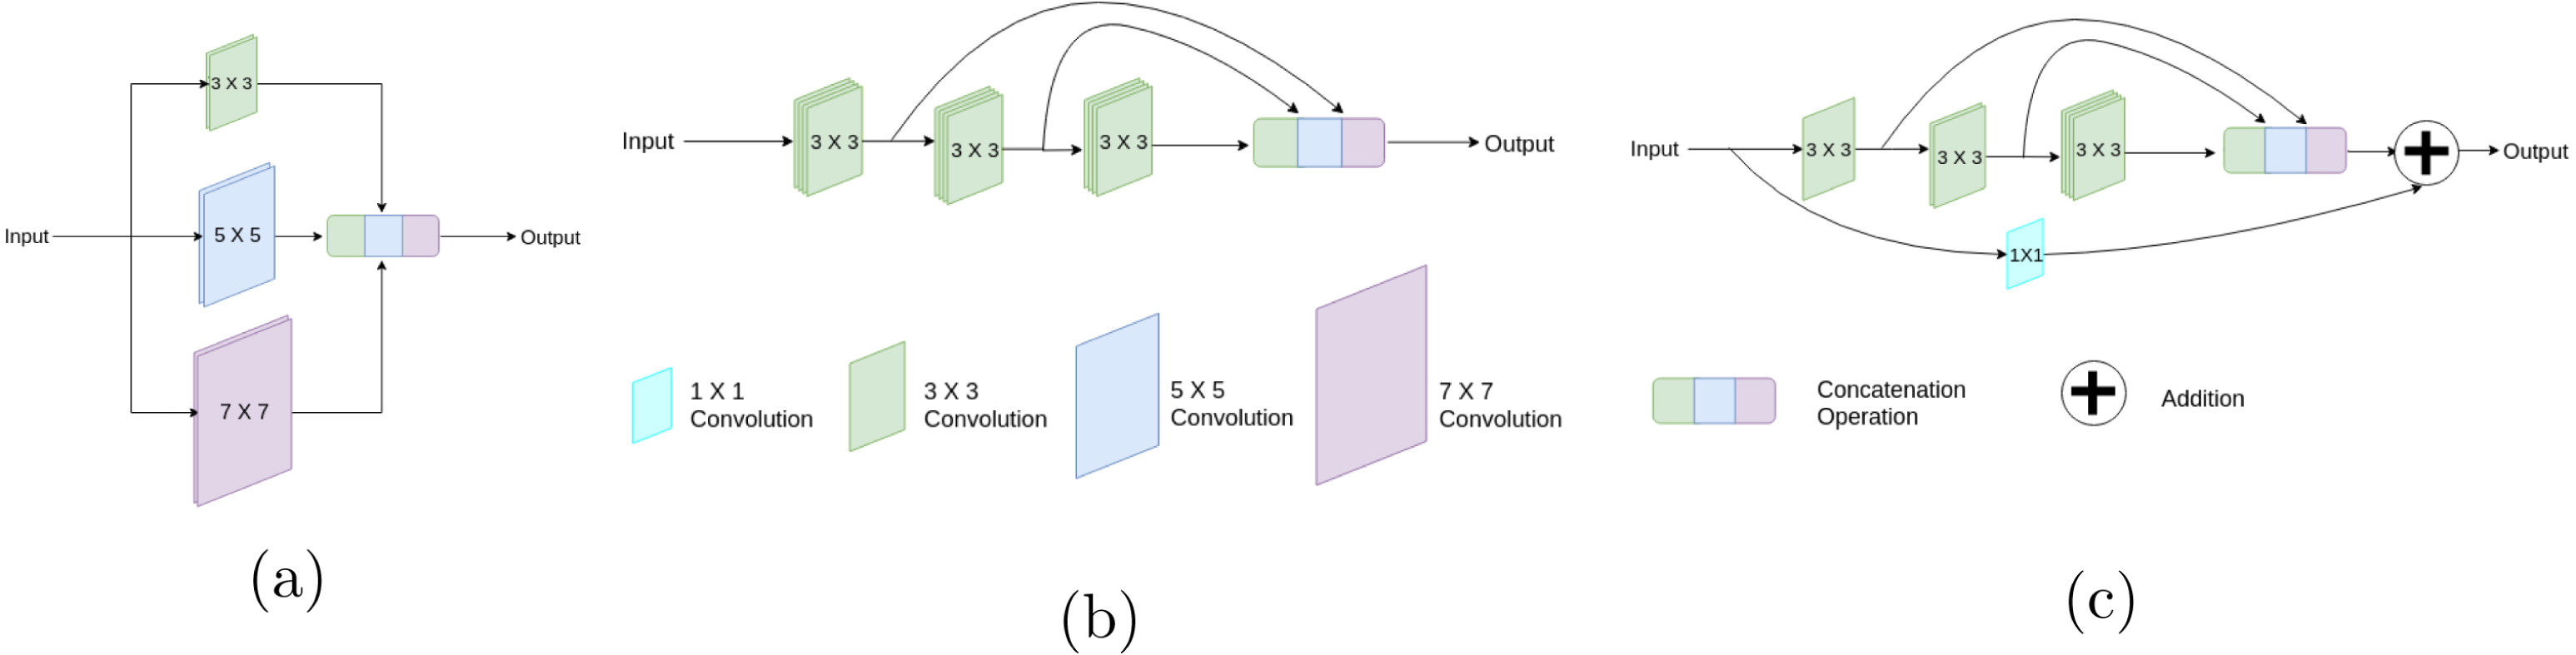
\includegraphics[width=1\columnwidth]{04-methodology/figures/multiresunet-multiresblock-steps.jpg}}
    \caption{Evalution of MultiRes block : \textbf{(a)} Inception-like block \textbf{(b)} a more expensive attempt \textbf{(c)} MultiRes block \cite{ibtehaz2020multiresunet}}
    \label{figure:multiresunet-multiresblock-steps}
\end{figure}

        Irregularity and images in different scales are common conditions in medical imaging samples.
        Neural networks aiming to get accurate results in medical imaging should able to overcome these kind of problems.
        Images in different scales is an ongoing situation for medical imaging even if there are some studies about it, because of that, it is not possible to say that this issue has been definitely resolved.
        \citet{szegedy2015going} proposed Inception architecure built on convolutional layers with various kernel size to minimize the difference of the scales between images.
        MultiResUNet has an improvement similar to Inception architecture.
        In addition to the 3x3 convolution layer in the classic U-Net, MultiResUnet has convolution layers in different kernels such as 5x5 and 7x7.
        Figure~\ref{fig:multiresunet-multiresblock-steps} shows the evolution of the MultiRes blocks with different attempts, resulting from the different uses of these kernels.
        These multires blocks have replaced the sequences of two convolutional layer in the vanilla U-Net.

        \begin{figure}
    \centerline{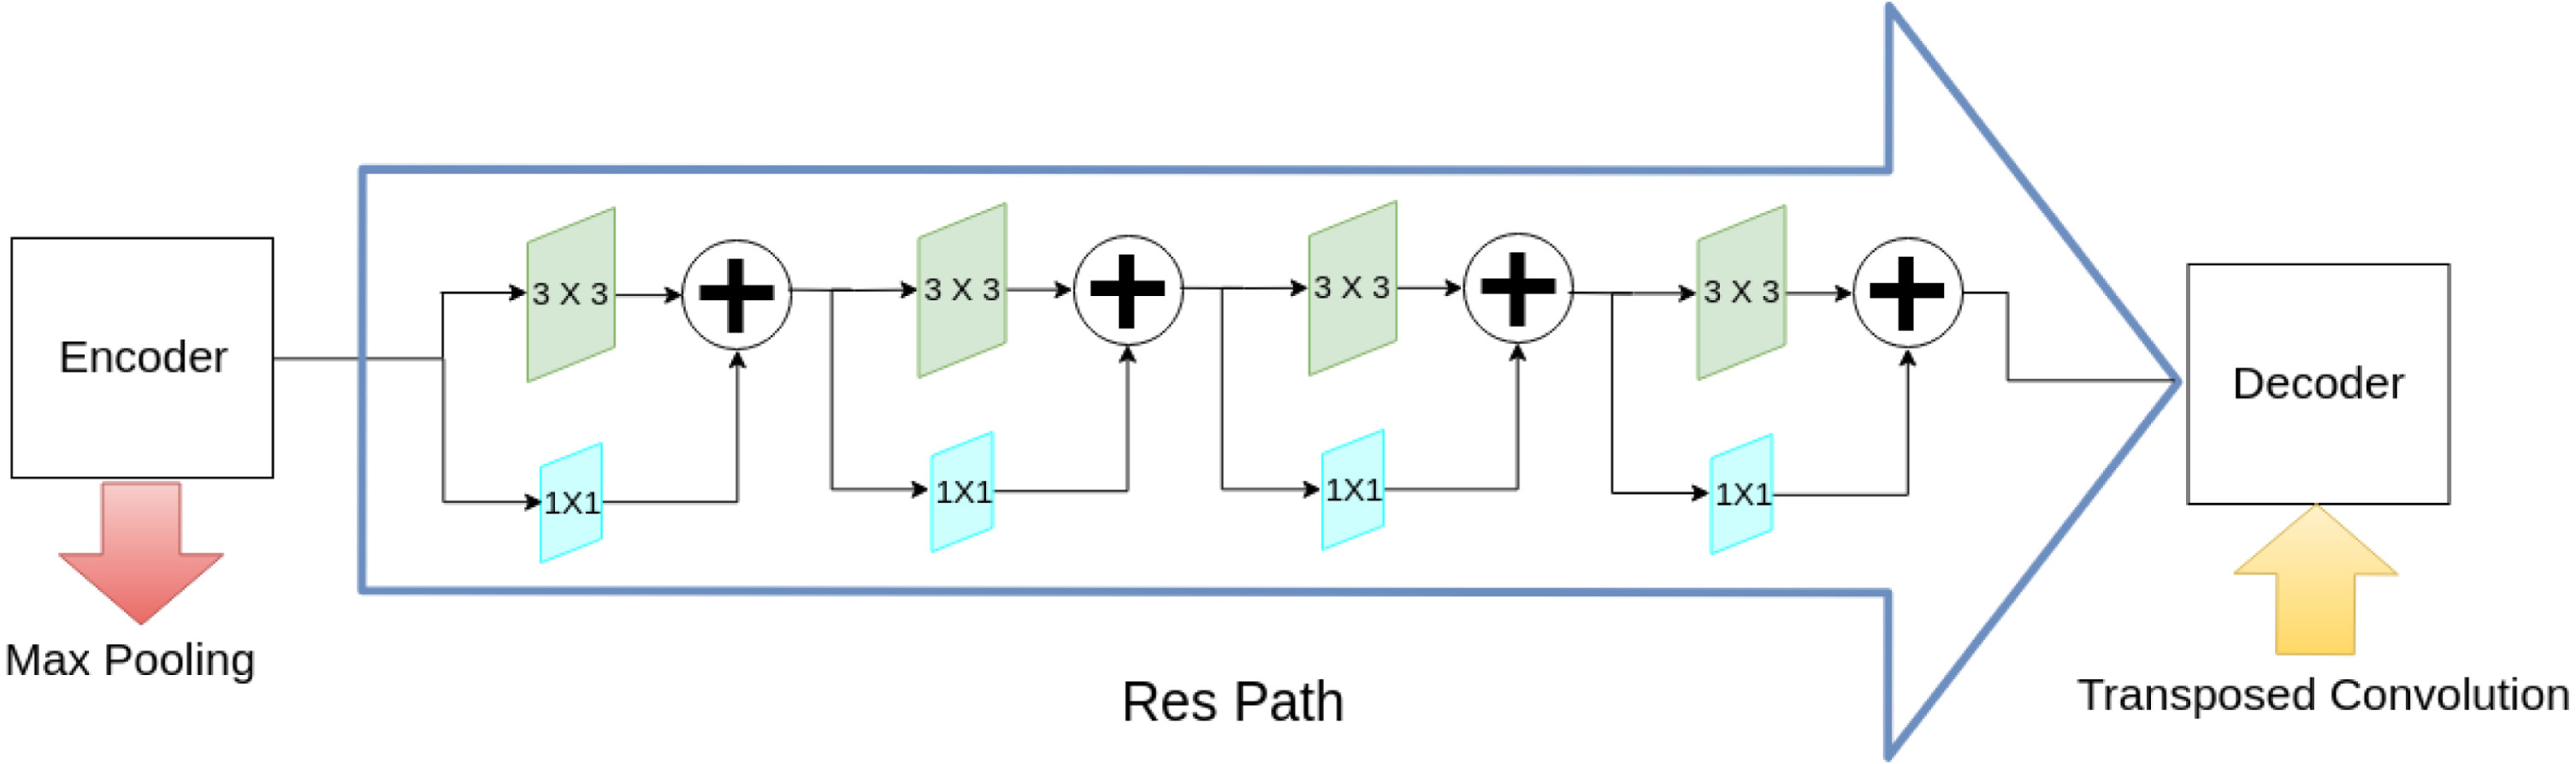
\includegraphics[width=1\columnwidth]{04-methodology/figures/multiresunet-respath.jpg}}
    \caption{Proposed Res path with residual connections \cite{ibtehaz2020multiresunet}}
    \label{fig:multiresunet-respath}
\end{figure}

        One of the significant improvement in U-Net is using the skip connections between the encoder and decoder.
        Thus, features which are lost during pooling is recovered and transferred from encoder to decoder.
        It is expected that the features sent by encoder to decoder are low level while the features in the decoder are expected to be high level.
        They thought that this may cause a semantic gap between the encoder and decoder and proposed another improvement called Res path which can be seen in Figure~\ref{fig:multiresunet-respath}.
        The proposed Res path consist of convolutional layers connected by residual connections to make learning easier \cite{drozdzal2016importance}.
        The features are being sent from encoder to decoder are transmitted over the Res paths instead of classical skip connections of U-Net.
        The proposed MultiResUNet framework is shown in Figure~\ref{fig:multiresunet-architecture} with the all improvements.

        \begin{figure}
    \centerline{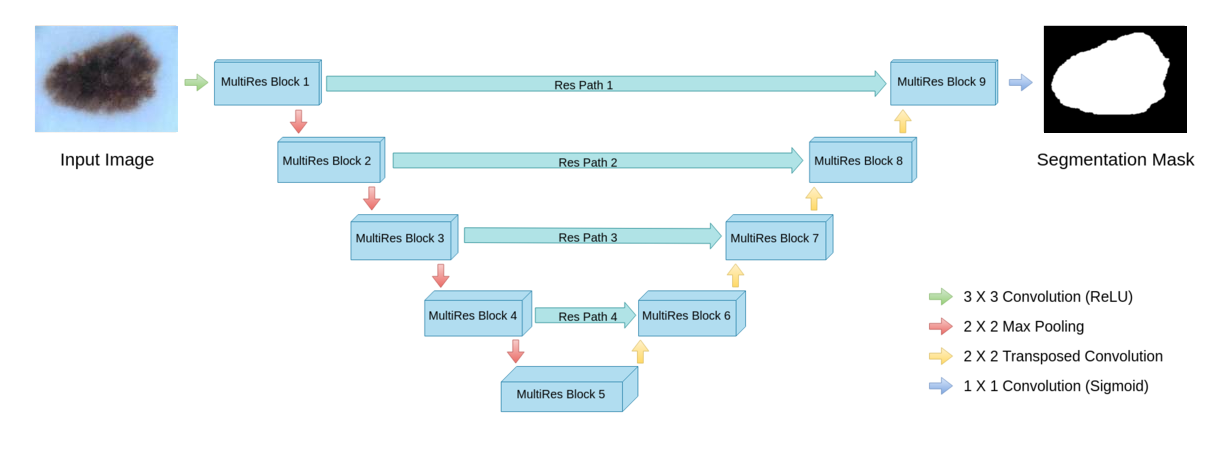
\includegraphics[width=1\columnwidth]{04-methodology/figures/multiresunet-architecture.png}}
    \caption{MultiResUnet architecture}
    \label{fig:multiresunet-architecture}
\end{figure}

        MultiResUNet has been tested and evaluated several dataset including Murphy lab, ISBI 2012, ISIC 2018, CVC-ClinicDB, and BraTS17
        with different modalities such as fluorescence microscopy, electron microscopy, dermoscopy, endoscopy, and MRI respectively.
        Their results show that the MultiResUNet offers more accurate results than the classical U-Net for the all 5 different datasets especially in dermoscopy and endoscopy images.

    \subsection{SegAN}\label{sec:segan}

        \citet{xue2018segan} proposed a new semantic segmentation network inspired by classical generative adversial networks (GANs).
        Their motivation about proposing a GAN based segmentation network is that there was no such GAN based network that give accurate results.
        \citet{luc2016semantic} have tried to segment images with a GAN-like network but explained that the network is unstable for image segmentation tasks.
        The creators of SegAN claim that the single scalar input, which is created by the discriminator,  may the reason of the unstability of image segmentation of conventional GANs.
        Because semantic segmentation requires pixel-level mapping, and the discriminator network of GAN may not be able to produce sufficient gradient feedback with single scalar output.
        The differences of the proposed network for semantic segmentation compared to classical GAN ​​are mentioned below.

        SegAN consists of two networks segmentor and critic similar to Generator and Discriminator networks of conventional GANs.
        It looks like a game as in GAN where the segmentor tries to fool the critic with the samples it creates.

        \begin{figure}
    \centerline{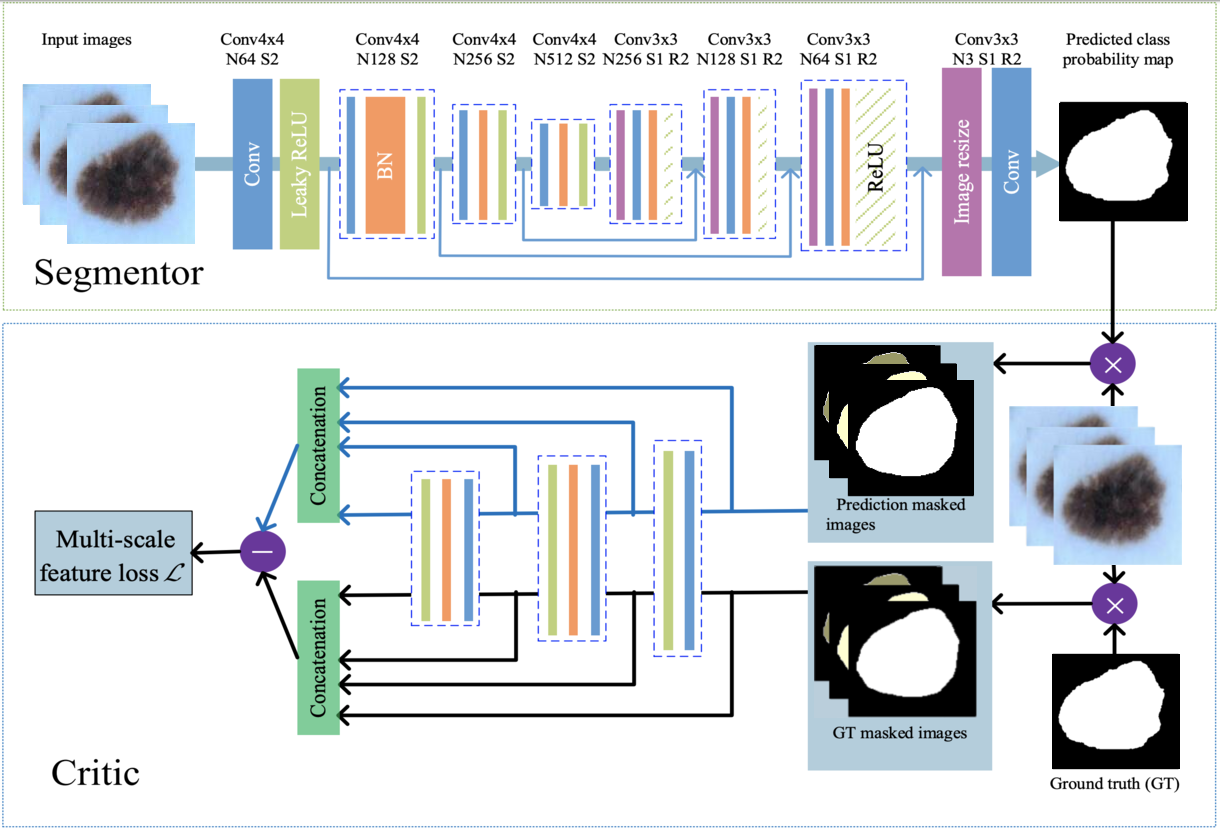
\includegraphics[width=1\columnwidth]{04-methodology/figures/segan-architecture.png}}
    \caption{SegAN architecture}
    \label{fig:segan-architecture}
\end{figure}

        The main difference comes with SegAN is multi-scale loss function. While two separate loss functions are defined for generator and discriminator in GAN,
        segmentor and critic use a common multi-scale loss function to force the both networks of SegAN to learn local and global features which acquires relations between pixels.

        The critic network aims to maximize multi-scale loss function using the differences of CNN features between the predicted images and the ground truth.
        On the other hand, segmentor network, which is an FCN, tries to minimize the loss function used in the critic network.
        They claim that the SegAN can learn spatial pixel features with the help of the proposed multi-scale loss function even the images are in different scales.

        SegAN is trained with the BRATS 2015 dataset and achieved remarkable results compared to other state-of-the-art models, including U-Net, in the field of semantic segmentation.


\section{Tools and Frameworks}

    This section presents tools used for development and testing during the thesis. Python is selected as the main programming language for this thesis.

    \textbf{Tools}

        \begin{itemize}

            \item \textbf{Numpy (Numerical Python)} is a scientific computing library for the Python that allows us
                    to perform scientific calculations quickly \cite{oliphant2006guide}. Numpy arrays form the basis of Numpy.
                    Numpy arrays are similar to Python lists, but are more useful in terms of speed and functionality than Python lists.

            \item \textbf{Scipy} is a package for scientific computing which includes functionality several clustering algorithms,
                    Fourier transforms, linear algebra, interpolation, regression, image and signal processing for the Python programming language \cite{virtanen2020scipy}.

            \item \textbf{Python Imaging Library (PIL)} is a free Python library which supports several widely-used image manipulation procedures
                    like per-pixed manipulating, image filtering, image enhancing, masking etc \cite{anjal2019roi}.

            \item \textbf{ImageMagick} is a open-source, free image editing tool that makes many morphological operation easy
                    for more than 200 image format with its built-in features like resize, flip, transform, or special filters \cite{ImageMag68online}.
                    It runs on multiple thread to increase performance and supports command-line usage that makes image editing possible for scripting languages.

            \item \textbf{Jupyter Notebook} is an open source web application that allows editing and running code
                    which can be used with over 40 different programming languages \cite{kluyver2016jupyter}.
                    It is a Json based document that has ordered cells which can be live code, equations, visualizations or narrative text.

        \end{itemize}

    \textbf{Deep Learning Frameworks}

        \begin{itemize}

            \item \textbf{TensorFlow} is an open source library for performing numerical computations. Although it can be used for computations in general,
                    it is most commonly used as a tool for machine learning research.
                    TensorFlow can be interfaced using Python and is then translated to a computational graph \cite{abadi2015tensorflow}.
                    The computational graph can be fed with the tensors  by launching a TensorFlow session which are generalization of N-dimensional arrays.
                    Weight matrices and biases are trainable variables in the TensorFlow graph during a session.
                    Loss functions and optimization algorithms for backpropagation exist in TensorFlow \cite{johansen2019medical}.
                    Therefore, training a model becomes as simple as specifying an objective function to optimize for, as well as running the optimizer with a batch of data inside a session.

            \item \textbf{Keras} is a neural networks API for Python \cite{chollet2015}. It runs on top of TensorFlow or Theano \cite{mohan2019medical}
                    which is used as the main neural network framework. Keras is user-friendly and allows for complex models to be created with relatively few lines of code.
                    Keras consists of many commonly used building blocks of neural networks. These are parts as layers, objectives, activation functions and optimizers.
                    The components include parts for convolutional and recurrent neural networks as convolutions, pooling, dropout and batch normalization.

            \item \textbf{PyTorch} is a machine learning framework introduced by Facebook which has relatively advantages over TensorFlow
                    in terms of simplicity and usability. It implements dynamic computational graphs which makes dynamic changes
                    on the networks possible with a little effort. Debugging is relatively easy with Pytorch.

        \end{itemize}


    \textbf{Hardware Requirements}

        Google Colab which is also known as Colaboratory that requires no setup and runs entirely in the cloud is used in this thesis.
            Colab is a Jupyter Notebook environment aims to support Machine Learning and Artificial Intelligence researches for free,
            because this kind of process requires serious computational power.
            Many deep learning projects can be developed with Google Colaboratory on the default GPU processor of it, Tesla K80, using common Deep Learning frameworks and tools like Keras,
            TensorFlow and PyTorch. Google Colab runs on a connected Google Drive accounts.
            All models were trained and tested using Tesla K80 GPU which has 25 GB of video memory on a Ubuntu 18.04.



\section{Experiments}

    Our study is composed of three steps; preprocessing, implementations of networks, and evaluation.
    During the preprocessing, image normalization procedures have been applied to data explained in Section~\ref{section:dataset};
    the image resizing and the conversion of file formats.
    Moreover, data size has been augmented by creating additional images files in different noise levels.
    Because our main focus is comparing the proposed network under the same conditions,
    the preprocessing stages were kept the same for a fair comparison of U-Net, MultiResUNet and SegAN.

    Hyperparameters of training proses are explained below while the compared networks are explained in details in Section~\ref{section:networks}.

    \begin{itemize}

        \item \textbf{Batch size} refers to the number of samples utilized in one iteration before updating the model parameters.
        It looks like an iteration where the error rate is calculated at the end of the iteration by comparing the batch predictions with ground truth.
        The calculated error is used to update model parameters.

        \item \textbf{Epoch} is an hyperparameters shows the number of passes of the algorithm through the entire training data.
        It depends on several criteria such as problem definition and data distribution and can changed from hundreds to thousands
        until the error rate of the learning algorithm reduced by a certain level.

        \item \textbf{Learning rate} determines how much an update step affects the current value of the model weights.
        In other words, it is used to decide how quickly the model will forget what it has already learned.

        \item \textbf{Optimizer}s try to minimize the loss function with the help of them by updating the model parameters.

    \end{itemize}

    U-Net and MultiResUnet have been trained for $200$ epochs with a batch size of $8$ and
    binary cross entropy loss function. As the performance did not increase epoch size has been kept as $200$.
    Adam optimizer has been used as optimizer with the default parameters stated in the original paper.

    Furthermore SegAN has been trained for $200$ epochs with a batch size of $200$ and an adaptive learning
    rate for Adam optimizer which started from $2.0 x 10^{-4}$ and multiplied by a decay rate of
    $0.5$ every $25$ epochs. Several learning and decay rates have been tried but the given parameters were found optimal like the original article.

    Early stopping has been used for the all networks.
    If the performances of models stoped improving after a certain number of epochs, $30$ was set to stop the training.

    The experiments have been designed by giving additive noise into initial dataset.
    Five different noise levels except to noise free have been tested using Gaussian noise given as it follows through the
    initial image $I_i$;

    \begin{equation}
        I_{final} = I_i + I_n \label{equation:noisy_common}
    \end{equation}

    $I_{final}$ and $I_{n}$ in Equation \eqref{equation:noisy_common} are the noisy image and Gaussian noise, respectively.

    The Gaussian noise is defined in the Equation  \eqref{equation:noise_gaussian}.

    \begin{equation}
        p_G(z) = \frac{1}{\sigma\sqrt{2\pi}} e^{ -\frac{(z-\mu)^2}{2\sigma^2} }  \label{equation:noise_gaussian}
    \end{equation}

    $p_G(z)$ denotes the noise distribution in single channel image.
    Our images have been encoded in RGB channels. Therefore, the noise has been applied for the all three channels.

    $\mu$ and $\sigma$ represents the mean value and the standard deviation, respectively.
    We used $5$ noise levels for the experiments with different $\sigma$ values from 0 to 50 by 10.

\section{Evaluation Metrics}

    Several evaluation metrics were used to determine the quality of the models.
    Dice coefficient, Jaccard index, Accuracy, Sensitivity and Specificity  were used to compare the target and predicted segmentation mask.
    The true positives (TP) determine pixels (or voxels) correctly classified as being part of the segmentation,
    a false positive (FP) is a pixel incorrectly classified as being part of the segmentation, and a false negative (FN)
    is a pixel which should have been part of the segmentation but was not.

    \begin{itemize}

        \item \textbf{Dice coefficient} which is also known as similarity coefficient or F1 score is a similarity metrics
                computed by comparing the pixel-wise agreement between the groundtruth and its predicted segmentation.
                Specially, this metric is just used to evaluate the segmentation performance of the model.

                \begin{equation}
                    Dice &= \frac{2 * TP}{2 * TP + FN + FP} \\
                \end{equation}

        \item \textbf{Jaccard index} also known as the Jaccard similarity coefficient, is a similarity metrics
                which compares predictions with the ground truths by dividing the size of the intersections by size of the unions.

                \begin{equation}
                    Jaccard &= \frac{TP}{TP + FN + FP} \\
                \end{equation}

        \item \textbf{Accuracy} measures the proportion of true positives and true negatives whose are correctly segmented instances
                to the total number of instances. It is derived from sensitivity and specificity which are given below.

                \begin{equation}
                    Accuracy &= \frac{TP + TN}{TP + FP + TN + FN} \\
                \end{equation}

        \item \textbf{Sensitivity and Specificity} are the other metrics used in this project. Sensitivity aims to measure
            correctly segmented instance ratio while specificity measures incorrectly segmented instance ratio.

                \begin{equation}
                    Sensitivity &= \frac{TP}{TP + FN} \\
                \end{equation}

                \begin{equation}
                    Specificity &= \frac{TN}{TN + FP} \\
                \end{equation}

    \end{itemize}




%
\chapter{Results}

    Experiments show that the both SegAN and MultiResUNet achieved almost the same dice coefficient result for the noise free images.
    MultiResUNet is slightly more successful than SegAN if they compared with Jaccard coefficient.
    The detailed results are given in the Table ~\ref{all-metrics-all-noises-segan} and Table ~\ref{all-metrics-all-noises-multiresunet} through statistical metrics.
    As can be seen from these tables, although the dice results of the models are very close for the noiseless datasets, the dice results differ as the noise level increases.

    The both models achieved their best results in about epoch of 50. The results are almost the same after that point.
    Figure ~\ref{fig:all-noises-by-epoch-dice-multiresunet} and Figure ~\ref{fig:all-noises-by-epoch-dice-segan} are point out the dice results of models at different epochs.

%    \sidebyside
%        {05-results/figures/segan/avg/ISIC_0012330.jpg}{Original image}
%        {05-results/figures/segan/avg/ISIC_0012330.png}{Ground truth}
%        {05-results/figures/segan/avg/ISIC_0012330_dice_8288.png}{Result(dice=0.82)}
%        {SegAN result with average score at 0\% of Gaussian noise}{fig:segan-avg-dice}

    \sidebyside
        {05-results/figures/segan/bad/ISIC_0012136.jpg}{Original image}
        {05-results/figures/segan/bad/ISIC_0012136.png}{Ground truth}
        {05-results/figures/segan/bad/ISIC_0012136_dice_5015.png}{Result(dice=0.50)}
        {SegAN result with low success compared to average at 0\% of Gaussian noise}{fig:segan-bad-dice}

    \sidebyside
        {05-results/figures/segan/good/ISIC_0012152.jpg}{Original image}
        {05-results/figures/segan/good/ISIC_0012152.png}{Ground truth}
        {05-results/figures/segan/good/ISIC_0012152_dice_9112.png}{Result(dice=0.91)}
        {SegAN result with high success compared to average at 0\% of Gaussian noise}{fig:segan-good-dice}

    \begin{figure}
    \centerline{\scalebox{0.55}{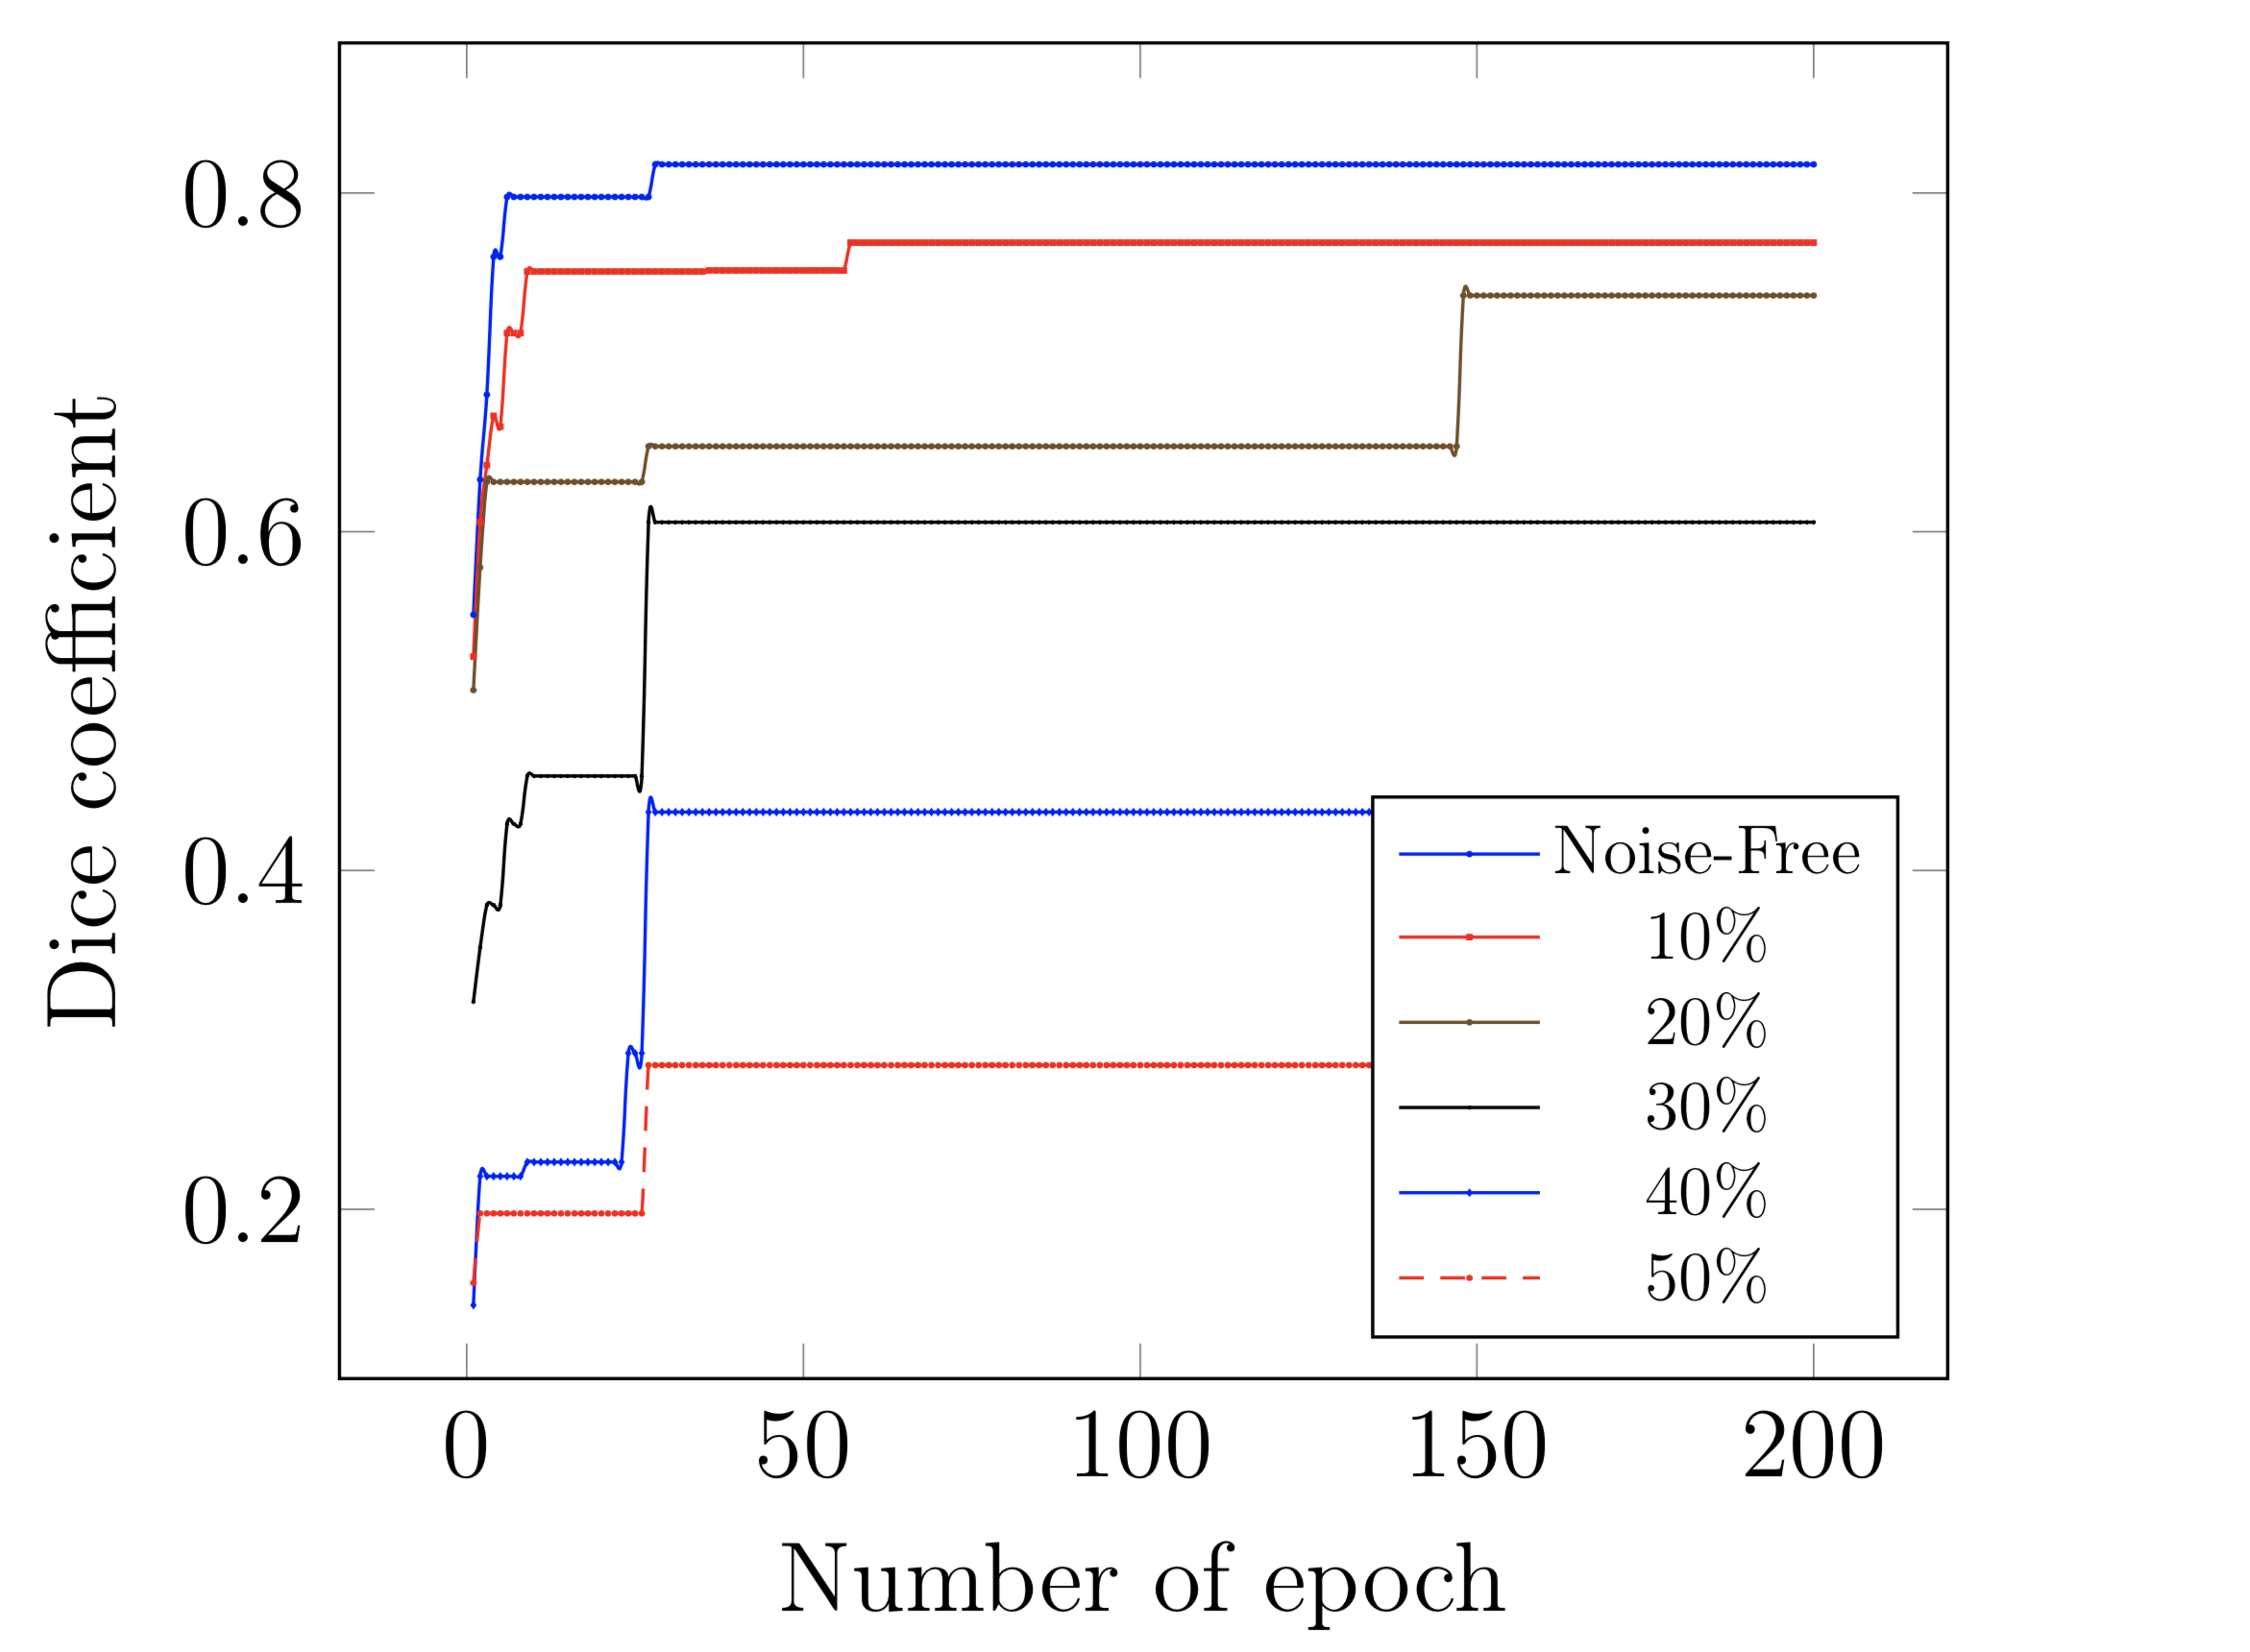
\includegraphics{05-results/figures/all-noises-by-epoch-dice-segan.png}}}
    \caption{Dice results for SegAN at different Gaussian noises by number of epochs}
    \label{fig:all-noises-by-epoch-dice-segan}
\end{figure}

%\figureallnoises
%    {05-results/plots/all-noises-by-epoch-dice-segan.txt}
%    {Dice results for SegAN at different Gaussian noises by number of epochs}
%    {fig:all-noises-by-epoch-dice-segan}


%    \sidebyside
%        {05-results/figures/multiresunet/avg/ISIC_0012152.jpg}{Original image}
%        {05-results/figures/multiresunet/avg/ISIC_0012152.png}{Ground truth}
%        {05-results/figures/multiresunet/avg/ISIC_0012152_dice_8048.jpg}{Result(dice=0.80)}
%        {MultiResUNet result with average score at 0\% of Gaussian noise}{fig:multiresunet-avg-dice}

    \sidebyside
        {05-results/figures/multiresunet/bad/ISIC_0012356.jpg}{Original image}
        {05-results/figures/multiresunet/bad/ISIC_0012356.png}{Ground truth}
        {05-results/figures/multiresunet/bad/ISIC_0012356_dice_543.jpg}{Result(dice=0.54)}
        {MultiResUNet result with low success compared to average at 0\% of Gaussian noise}{fig:multiresunet-bad-dice}

    \sidebyside
        {05-results/figures/multiresunet/good/ISIC_0012092.jpg}{Original image}
        {05-results/figures/multiresunet/good/ISIC_0012092.png}{Ground truth}
        {05-results/figures/multiresunet/good/ISIC_0012092_dice_904.jpg}{Result(dice=0.90)}
        {MultiResUNet result with high success compared to average at 0\% of Gaussian noise}{fig:multiresunet-good-dice}

    When the noise level is 50\%, the dice results of MultiResUNet's decreased up to 28\%, while the SegAN's decreased up to 53\%.
    As it explained in Section ~\ref{sec:multiresunet}, SegAN introduces fake skin lesions during the generator level and the discriminator takes a decision after the training if test image is a lesion.
    The noise added during the training phase of SegAN makes the model more successful againist noisy data.

    Figure ~\ref{fig:comparision-of-models-for-noise-tolerance} shows the change of success of the models against noise.
    As can be seen here, SegAN is more robust than MultiResUNet at increased levels of Gaussian noises.


    \begin{figure}
    \centerline{\scalebox{0.55}{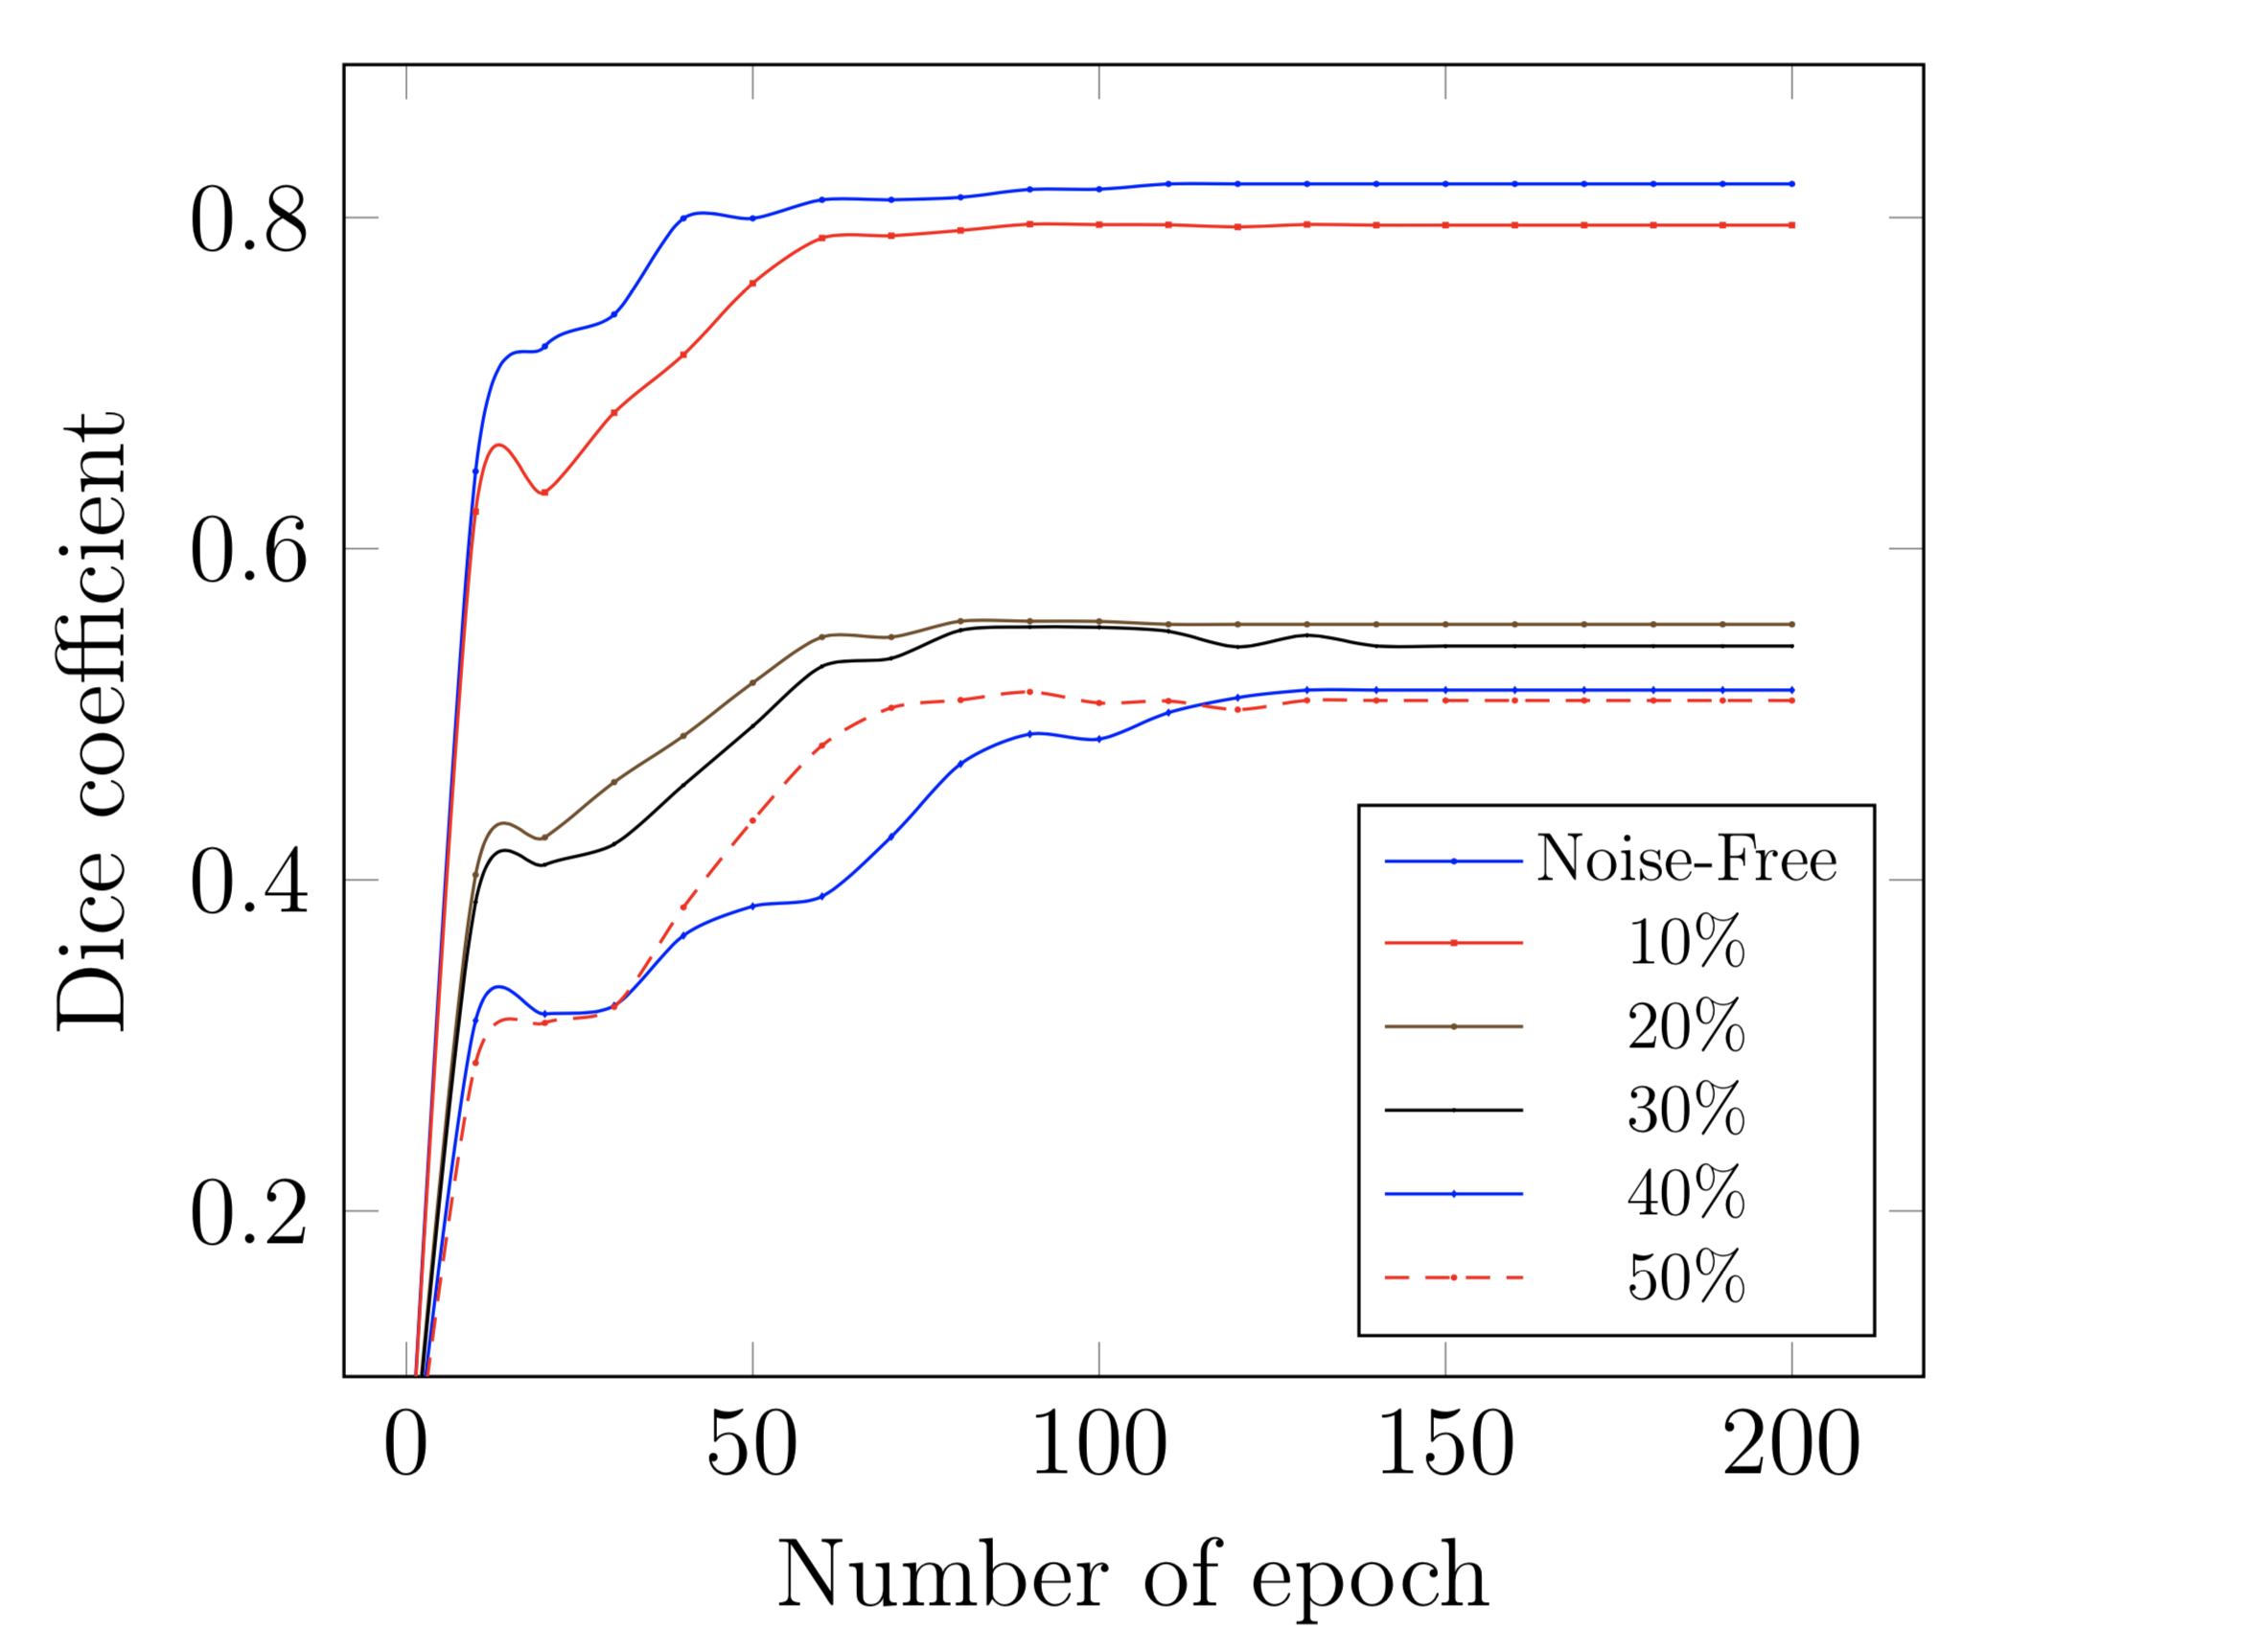
\includegraphics{05-results/figures/all-noises-by-epoch-dice-multiresunet.png}}}
    \caption{Dice results for MultiResUNet at different Gaussian noises by number of epochs}
    \label{fig:all-noises-by-epoch-dice-multiresunet}
\end{figure}

%\figureallnoises
%    {05-results/plots/all-noises-by-epoch-dice-multiresunet.txt}
%    {Dice results for MultiResUNet at different Gaussian noises by number of epochs}
%    {fig:all-noises-by-epoch-dice-multiresunet}

    \begin{table}[h]
\caption{Comparision of segmentation results of SegAN at different levels of Gaussian noise with evaluation metrics}
\centering
\begin{tabular}{c|ccccc}
Gaussian noise(\%)   & Dice   & Jaccard & Accuracy & Sensitivity & Specificity \\
\specialrule{2pt}{1pt}{1pt}
0   & 0.8110   & 0.6968  & 0.9236 & 0.8998 & 0.9240      \\
10  & 0.5570   & 0.4     & 0.8129 & 0.6232 & 0.8445      \\
20  & 0.5518   & 0.3936  & 0.8134 & 0.6322 & 0.8417      \\
30  & 0.5456   & 0.3878  & 0.8132 & 0.6329 & 0.8398      \\
40  & 0.5378   & 0.3791  & 0.809  & 0.6085 & 0.8442      \\
50  & 0.5368   & 0.3783  & 0.8115 & 0.6364 & 0.8351      \\
\hline
\end{tabular}
\label{all-metrics-all-noises-segan}
\end{table}

    \begin{table}[h]
\caption{Comparision of segmentation results of MultiResUNet at different levels of Gaussian noise with evaluation metrics}
\centering
\begin{tabular}{c|ccccc}
Gaussian noise(\%)   & Dice   & Jaccard & Accuracy & Sensitivity & Specificity \\
\specialrule{2pt}{1pt}{1pt}
0  & 0.8169 & 0.7221 & 0.922  & 0.964  & 0.9482 \\
10 & 0.7707 & 0.6747 & 0.9058 & 0.8923 & 0.9024 \\
20 & 0.7395 & 0.624 & 0.8829 & 0.8788 & 0.8705 \\
30 & 0.6056 & 0.4784 & 0.6056 & 0.8402 & 0.7949 \\
40 & 0.4345 & 0.3061   & 0.8062 & 0.7033 & 0.8104 \\
50 & 0.2851 & 0.1969 & 0.7878 & 0.7729 & 0.7847 \\
\hline
\end{tabular}
\label{all-metrics-all-noises-multiresunet}
\end{table}

    \begin{figure}
    \centerline{\scalebox{0.55}{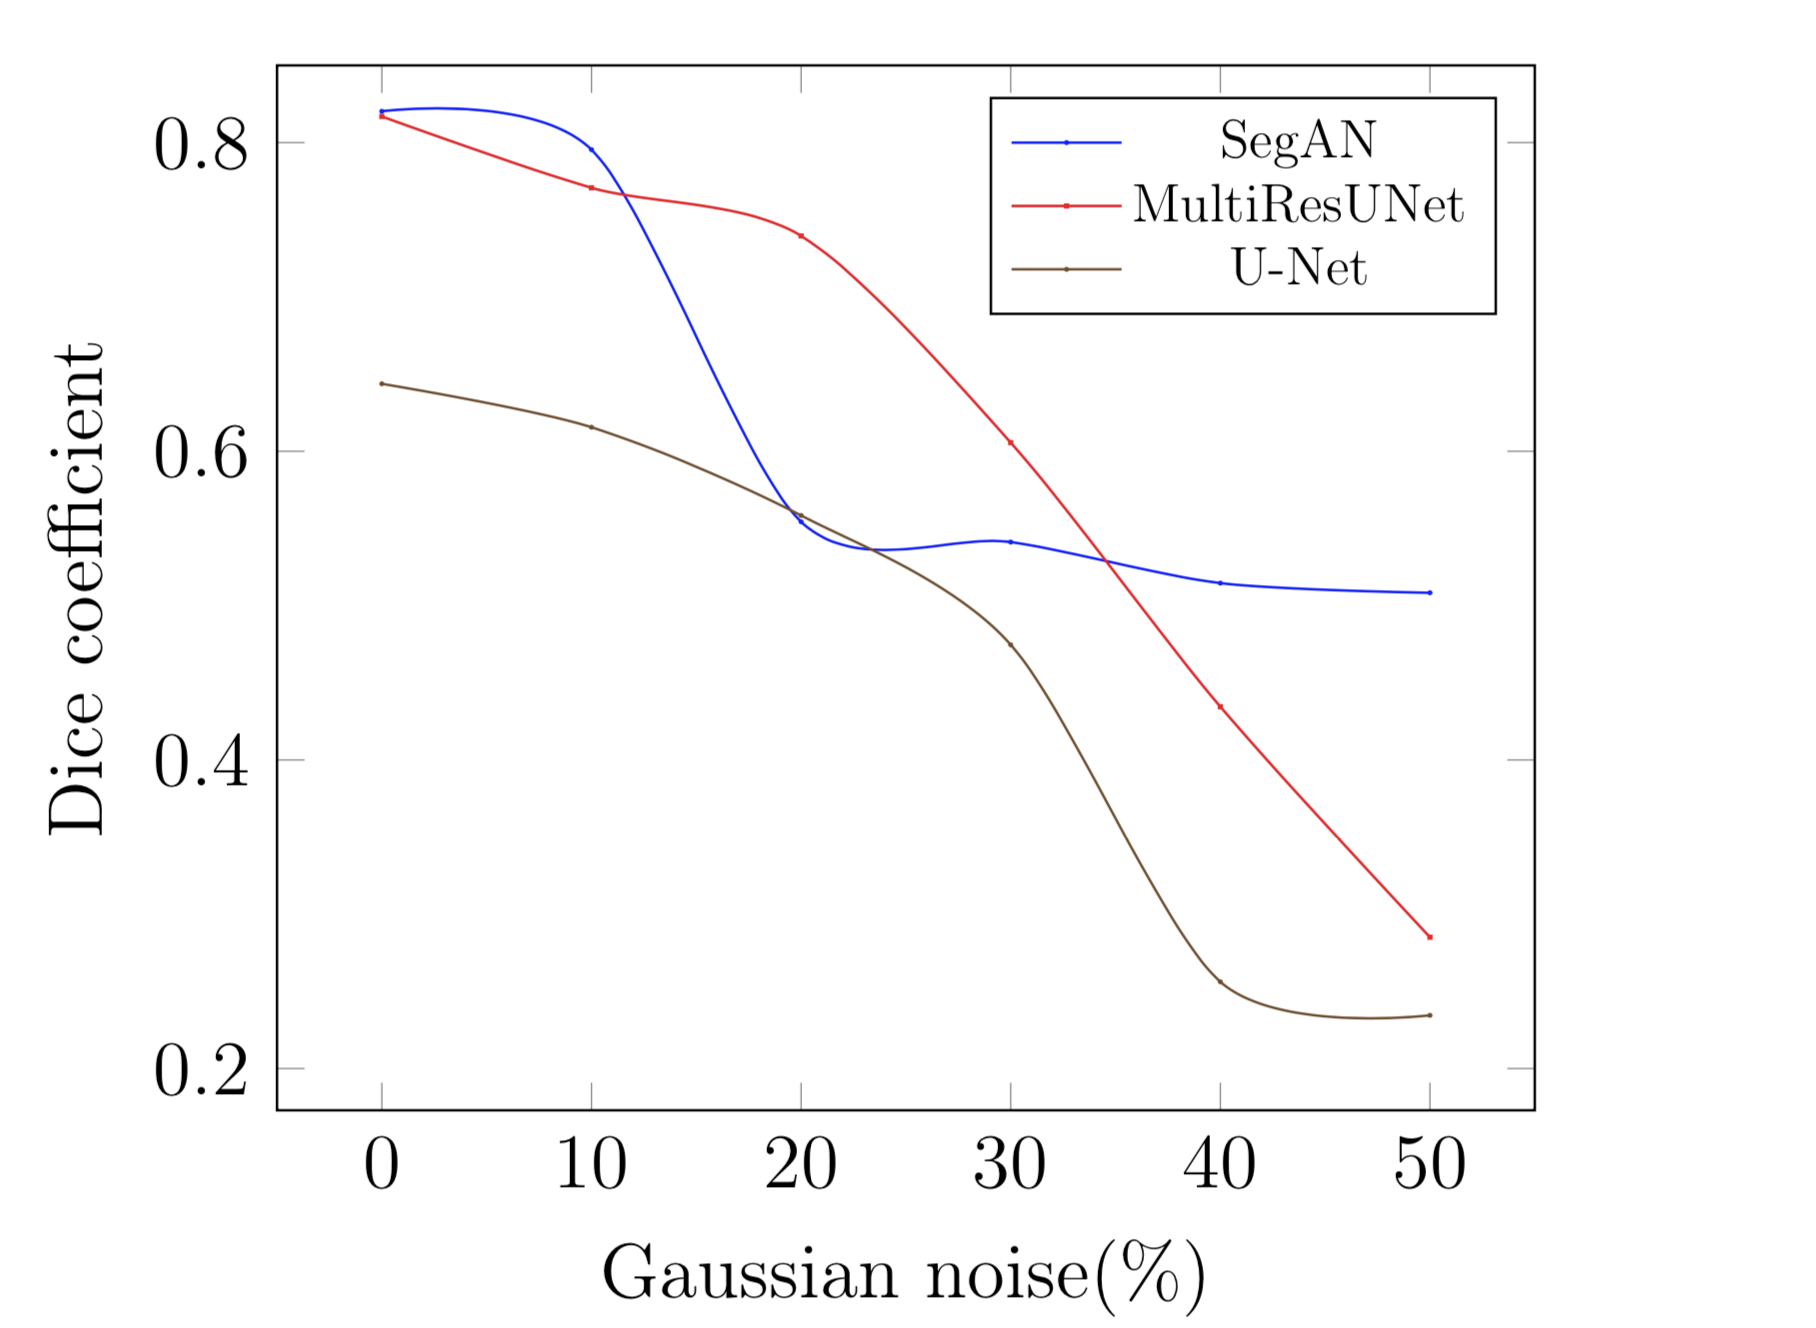
\includegraphics{05-results/figures/comparision-of-results-of-models-at-different-noise-levels.png}}}
    \caption{Comparision of the results of the models at different noise levels}
    \label{fig:comparision-of-results-of-models-at-different-noise-levels}
\end{figure}

%\figureavgnoises
%    {05-results/plots/dice-scores-with-different-gaussian-noise.csv}
%    {Dice result for SegAN at different Gaussian noises}
%    {fig:noise-tolerance-dice-segand}


    \begin{figure}
    \centerline{\scalebox{0.55}{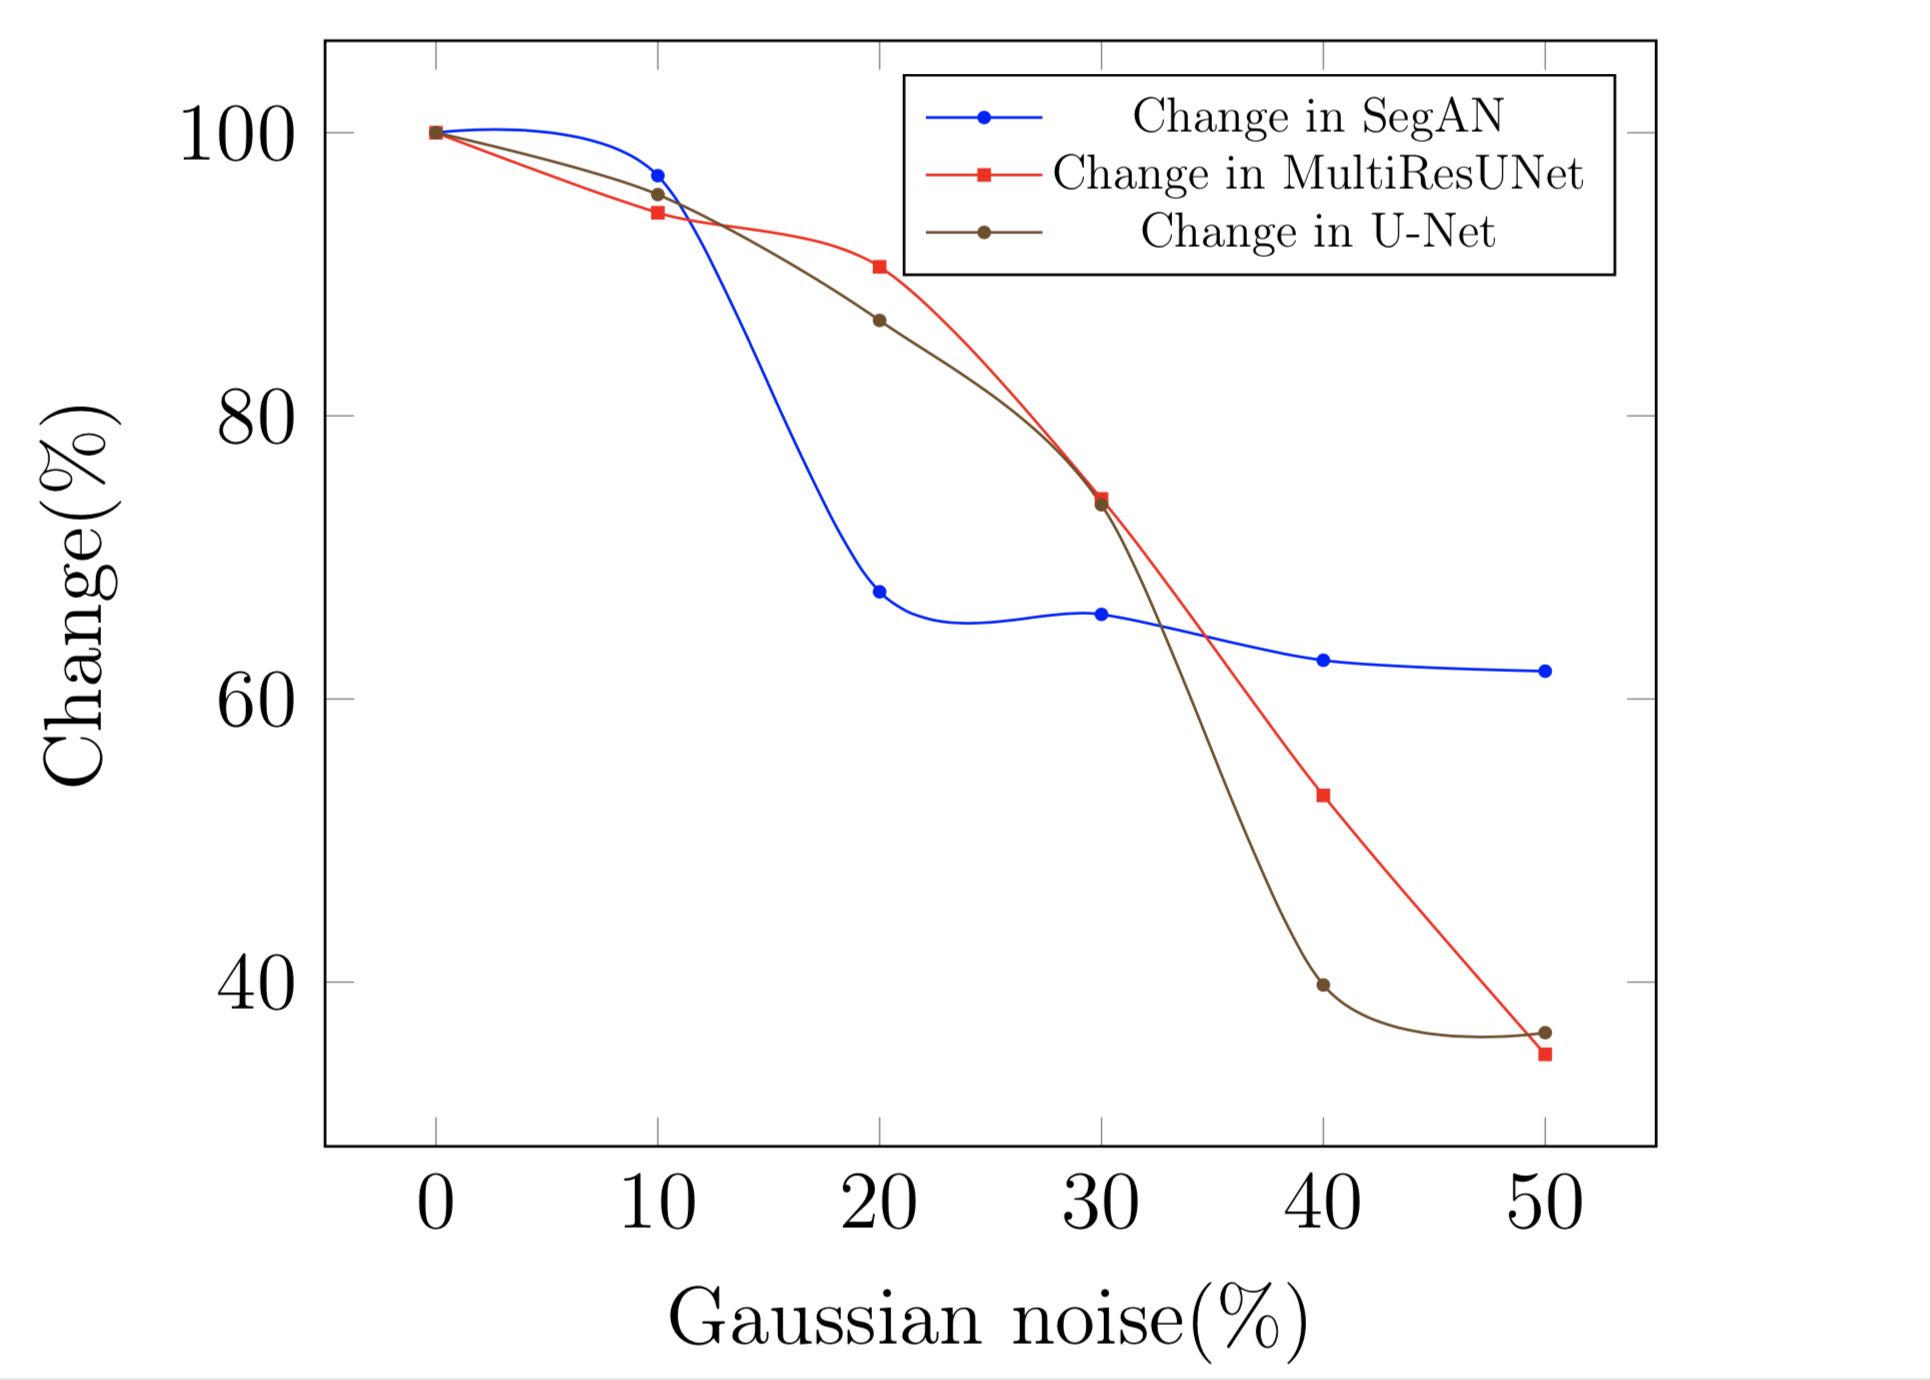
\includegraphics{05-results/figures/comparision-of-models-for-noise-tolerance.png}}}
    \caption{Change of success of the models by noise level}
    \label{fig:comparision-of-models-for-noise-tolerance}
\end{figure}

%\figuretolerancenoises
%    {04-methodology/plots/dice-scores-with-different-gaussian-noise.csv}
%    {Change of success of the models by noise level}
%    {fig:noise-tolerance-dice-seganda}

    \begin{figure}
    \centerline{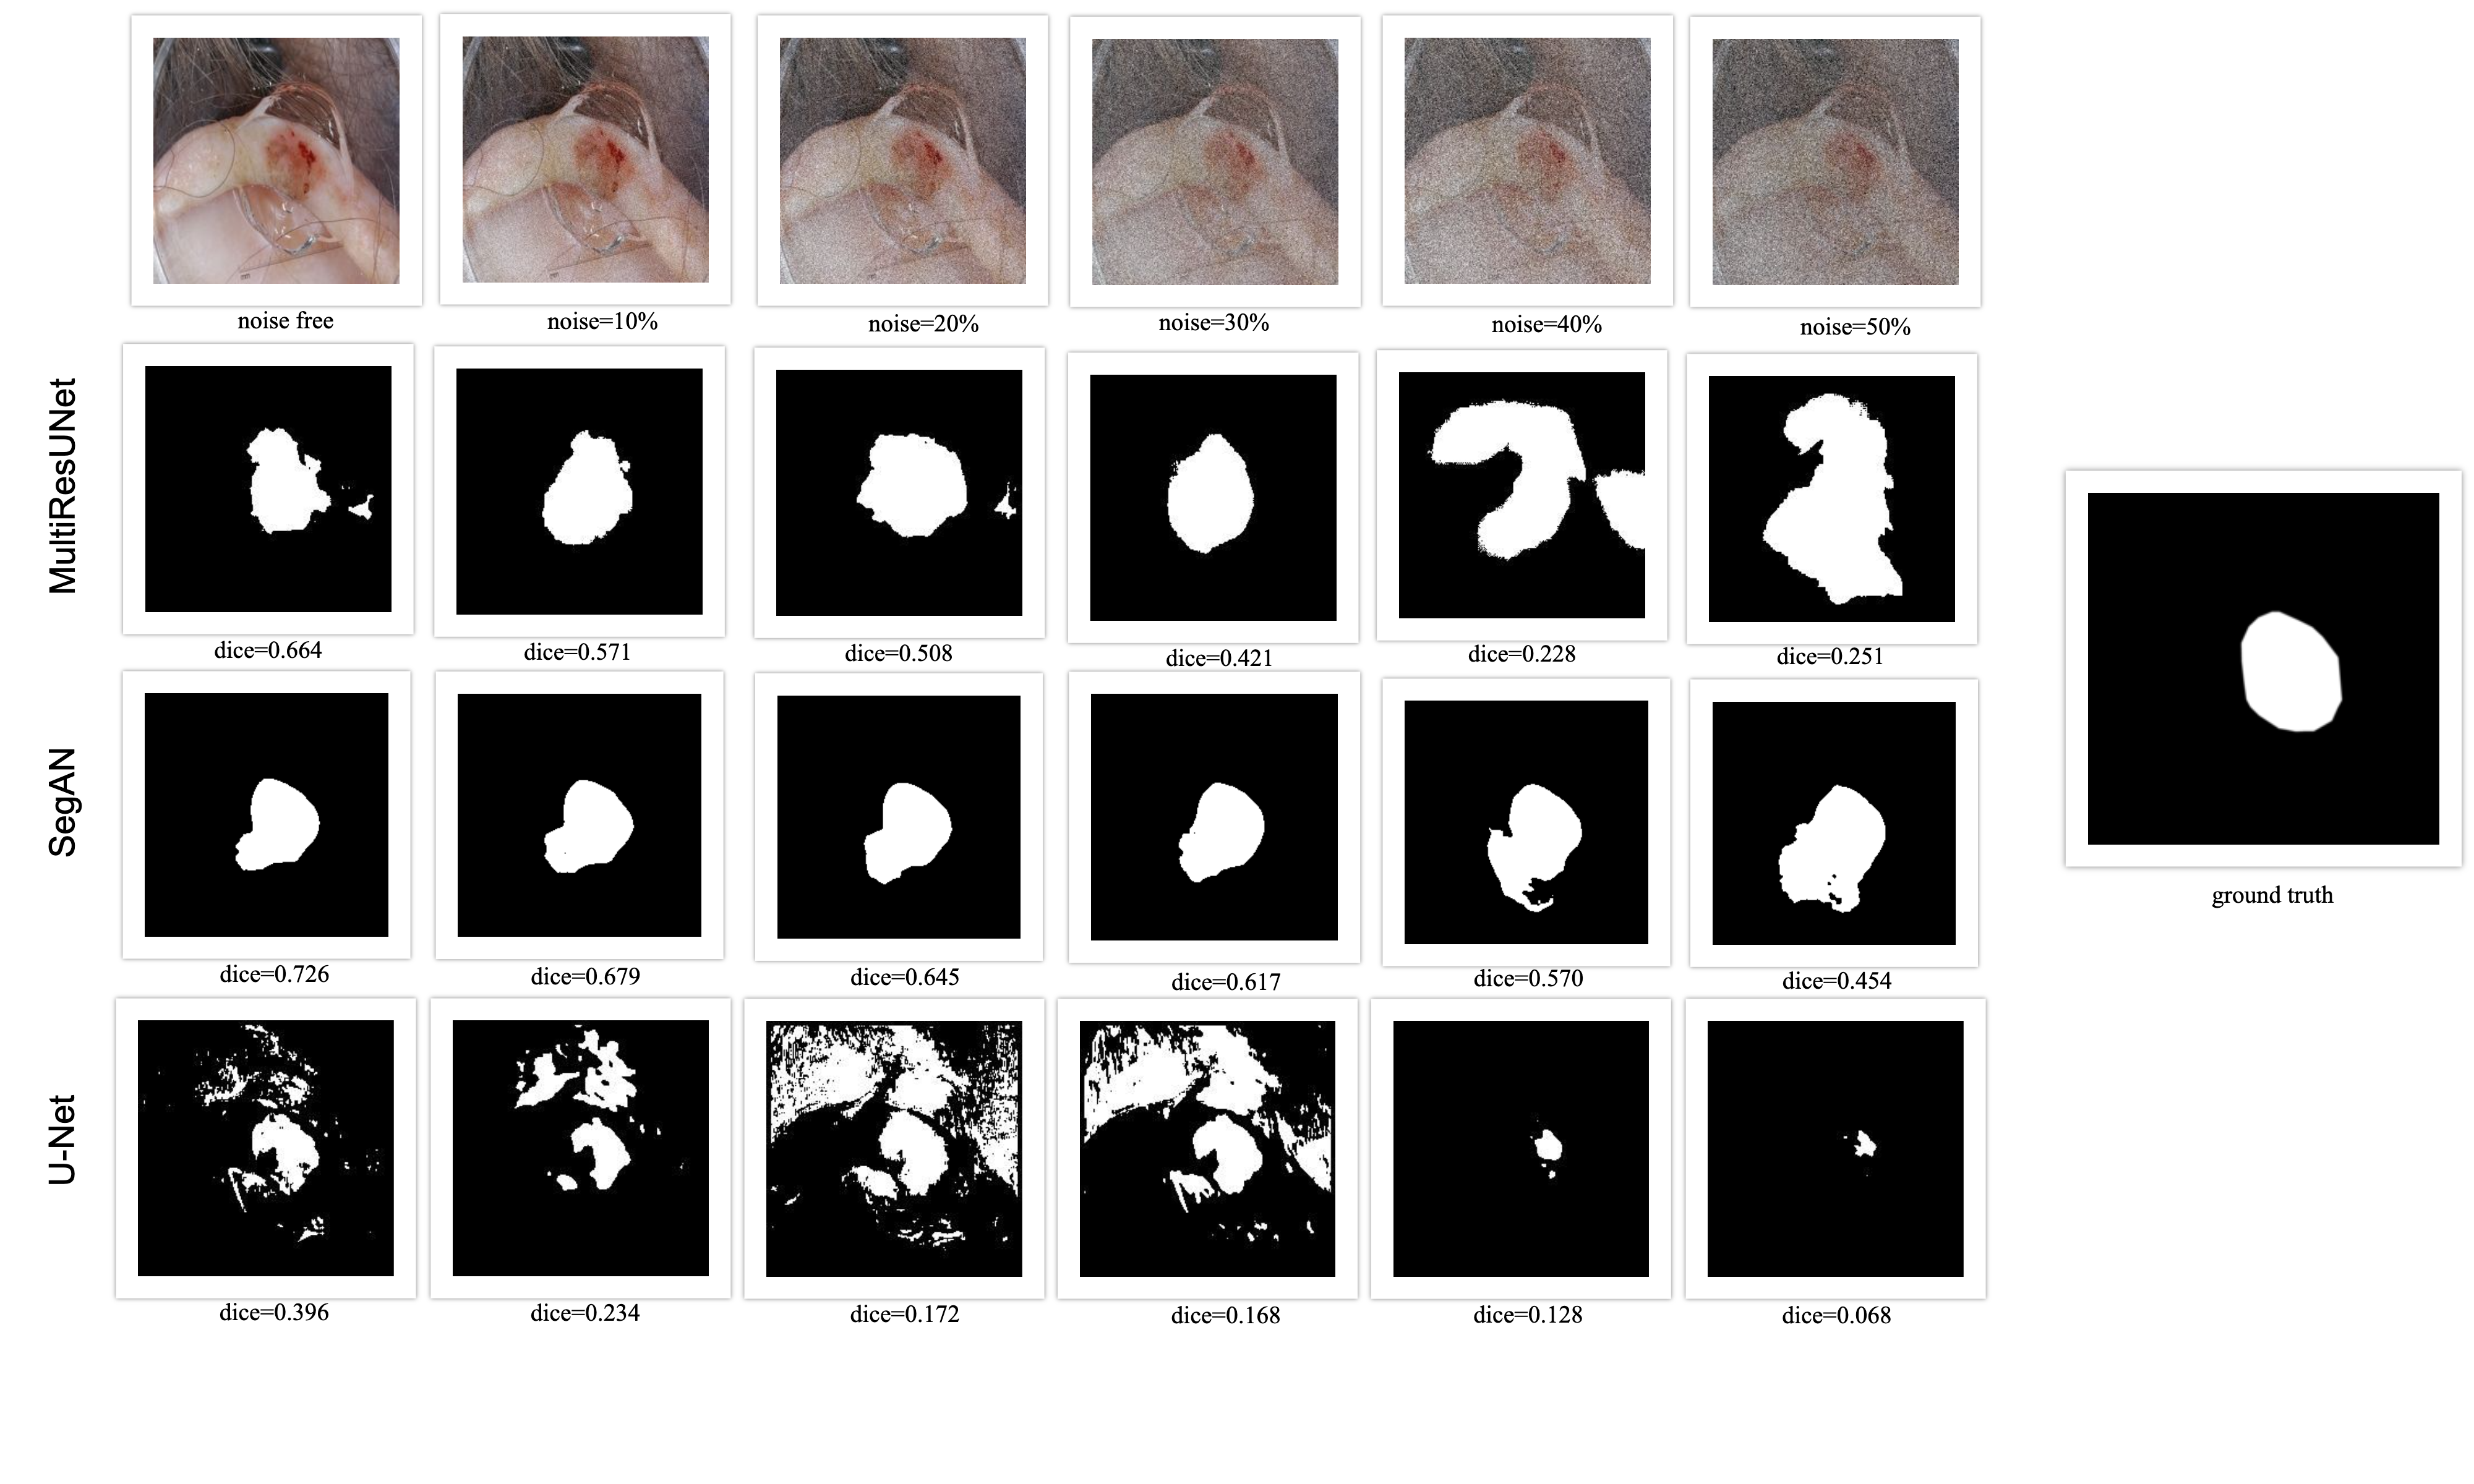
\includegraphics[width=1\columnwidth]{05-results/figures/extended_results_sample_gan_over_unet.png}}
    \caption{Dice results of the same image for SegAN and MultiResUNet at different Gaussian noises. The images in a column from top to bottom show the input, MultiResUnet result and SegAN result respectively. SegAN has better results.}
    \label{fig:all-noises-with-results-dice-segan-over-multiresunet}
\end{figure}


    \begin{figure}
    \centerline{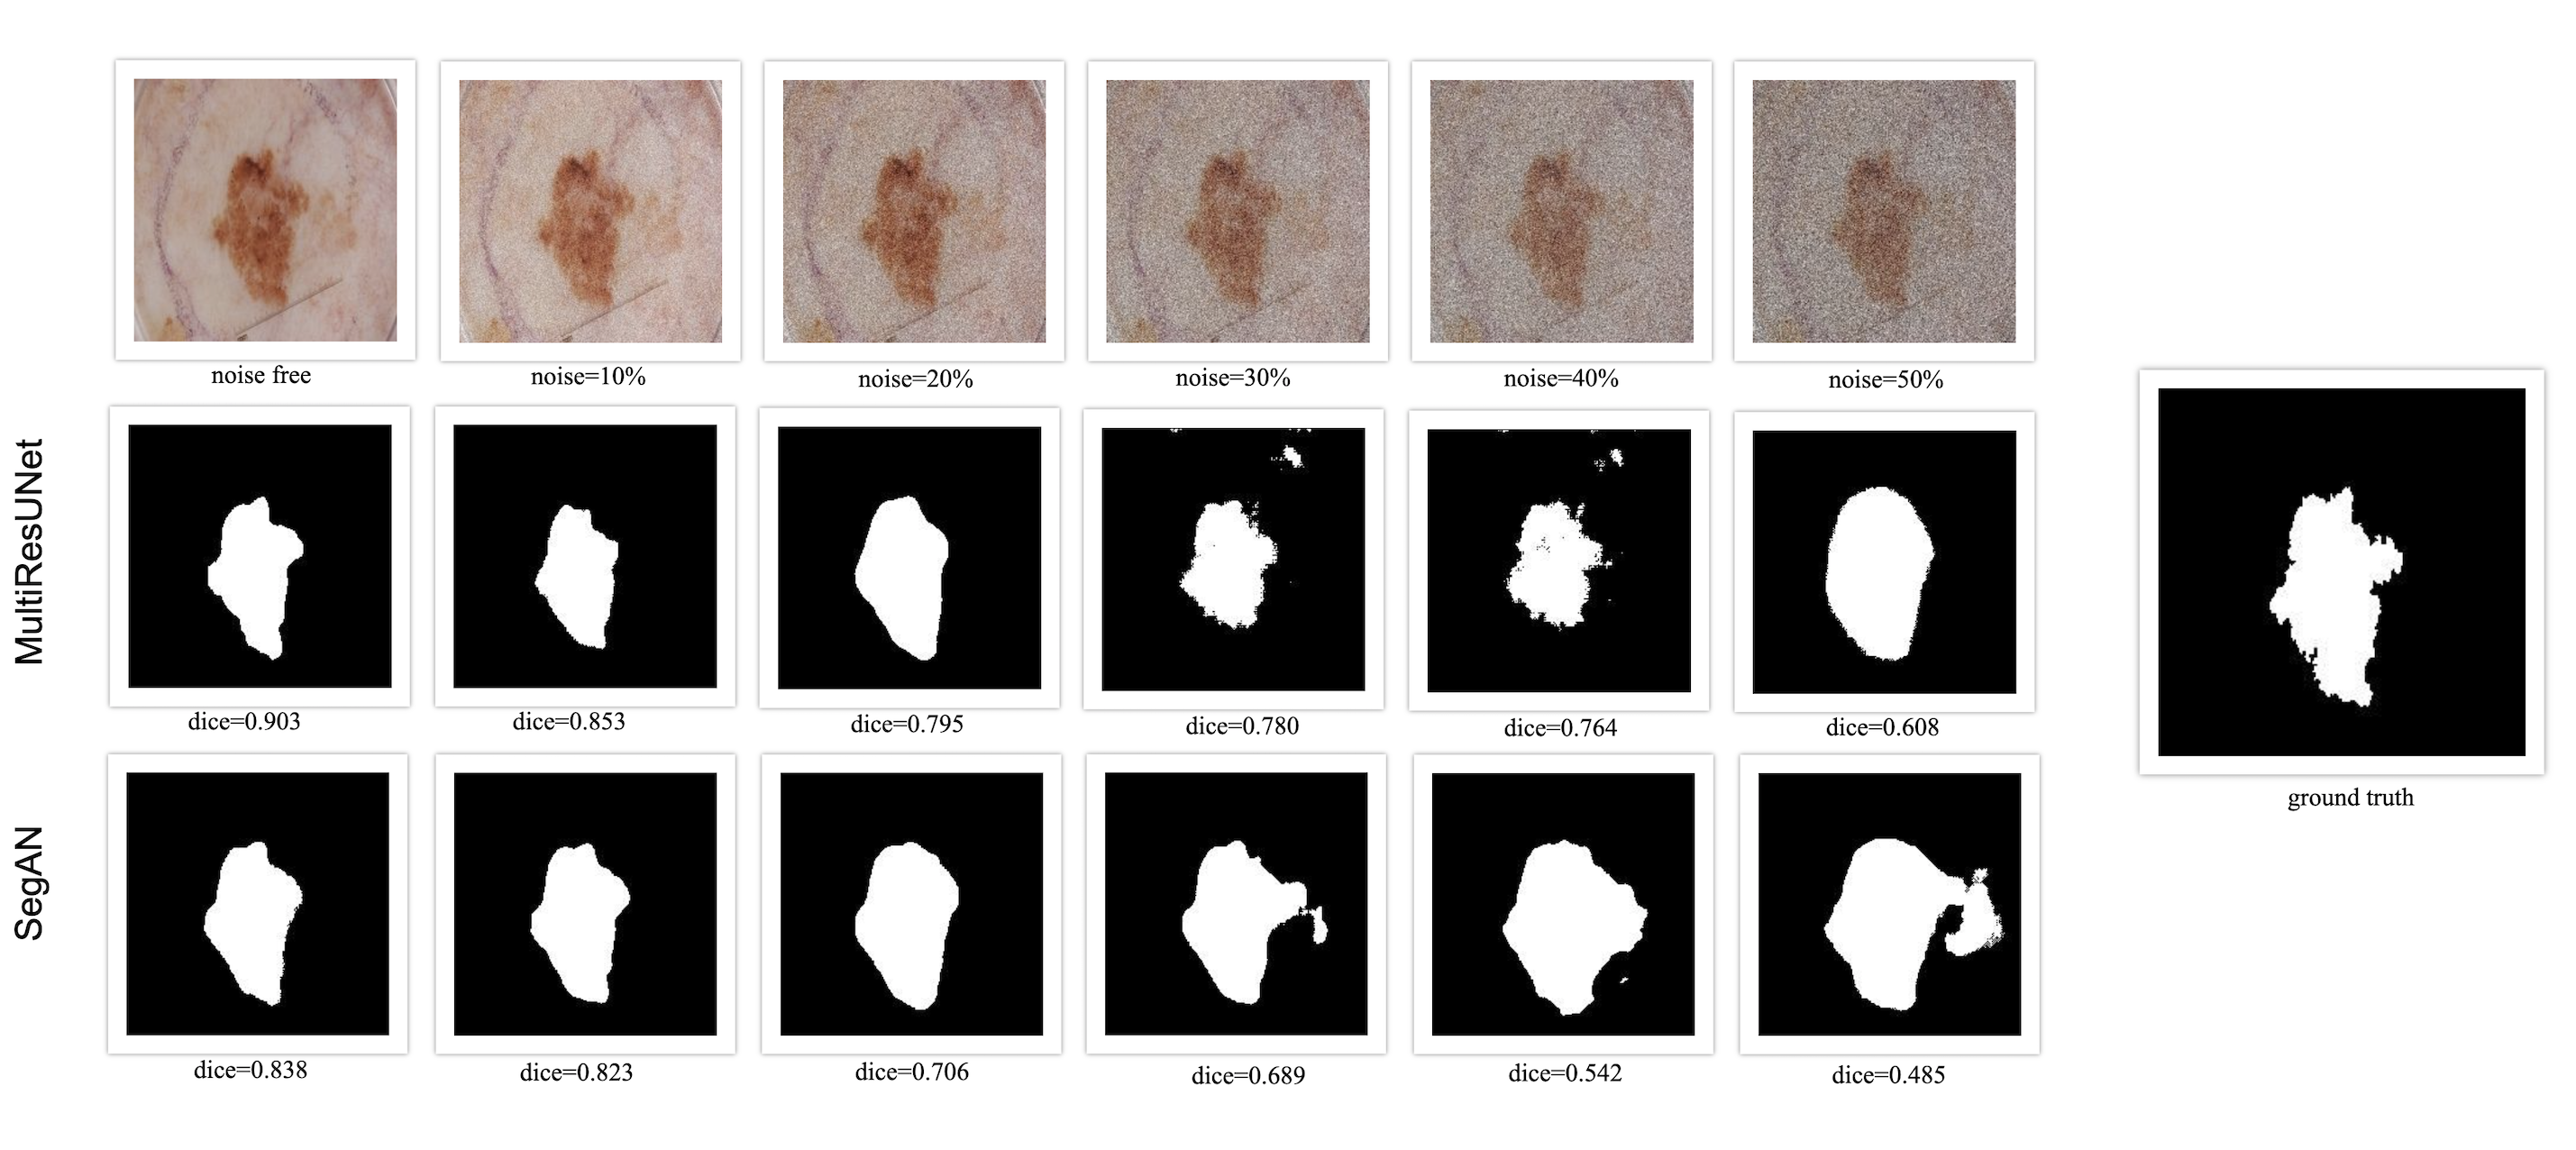
\includegraphics[width=1\columnwidth]{05-results/figures/extended_results_sample_unet_over_gan.png}}
    \caption{Dice results of the same image for the all networks at different Gaussian noises. The images in a column from top to bottom show the input, results of MultiResUnet, SegAN, and U-Net respectively. U-Net has better results}
    \label{figure:all-noises-with-results-dice-multiresunet-over-segan}
\end{figure}




    Although it is not possible to create a model that fit all dataset, it is the main objective to present a model that best generalizes them
    Figures ~\ref{fig:all-noises-with-results-dice-segan-over-multiresunet} and Figure ~\ref{fig:all-noises-with-results-dice-multiresunet-over-segan}
    are the outputs obtained by evaluating 2 pictures with two models in different levels of noises.
    While SegAN give more successful results for the image in Figure ~\ref{fig:all-noises-with-results-dice-segan-over-multiresunet},
    MultiResUNet is more successful in the image of Figure ~\ref{fig:all-noises-with-results-dice-multiresunet-over-segan}.
    As can be seen from that comparision, there is no precise superiority of the models to each other for certain data.


%
\chapter{Discussion}

    The architectures used in this thesis are those that have proven their worth in their fields.
    We aimed to examine both their success to Gaussian noise and their superiority against each other by comparing them with different Gaussian noise levels.
    In the MultiResUNet architecture, the most significant improvement compared to U-Net was the multi-scale loss function.
    Since our main purpose in our study was to compare models with each other, we did not need to compare these models with U-Net.
    Tests at different noise levels can also be done with U-Net to be able to see how well the models behave by well-known comparision point.
    On the other hand, all models can be subjected to more detailed pre and post processing steps.
    It can be understood whether the models are successful only in medical images by testing all of them with different datasets.

    Because it is not our main purpose to improve the model success, we did not update the inner configurations of models.
    In this context, adding different noises to relevant points in networks such as activation functions,
    loss functions, weights or hidden layers can be sensible to see the results of these kind of circumstances.

    Instead of choosing FCN as the segmentor network of SegAN architecture, we can replace it with MultiResUNet to see how powerful a new combined model is.
%
\chapter{Conclusion}

    In skin cancers, tumors may deady and early detection can increase the survival rate.
    Advanced technologies such as deep learning are used in several fields in medicine to increase the diagnosis of the illnesses in the early stages.
    Image based analysis can help to the oncologists or the surgeons when detecting the skin tumors.
    It is clearly stated that the main purpose of the deep learning in medical imaging is to help to the medicians instead of replacing them.
    These kind of supportive methods can help to the medicians before their final diagnosis.

    In this thesis, we have addressed the problem of skin lesion segmentation, providing a unified comparision between several  state-of-the-art deep learning methods
    for medical image segmentation namely Capsule Network, SegAN, and MultiResUNet.
    The comparision dataset is acquired from ISIC 2017 Challenge and enriched by adding Gaussian noises at different levels of sigmas.
    Insufficient data is a big challenge in medical imaging and this thesis aimed to provide accurate guidance, even if the dataset is insufficient.
    The experiment results showed that none of them is superior to others for the all dataset.

%
% End of Chapters
%

\bibliography{99-util/bibliography}
\bibliographystyle{dcu}

\appendix
\thispagestyle{empty}

    \chapter[]{Proof of Some Theorem}
    \thispagestyle{empty}

\curriculumvitae
\label{chapter:vita}

Fatih Ergin was born on August 7, 1991 in Gümüşhane, Turkey.
He completed his high school education at Erzincan Anatolian Teacher High School in 2009.
He obtained his bachelor degree in Computer Engineering with his study on
"Collaborative Filtering Based Recommendation Systems" from Istanbul Technical University, Turkey in 2014.


\section*{\uppercase{Publications}}

    \begin{itemize}
        \item[] Ergin, F., Parlak, B. (2020). A Deep Learning Model for Skin Lesion Analysis using Generative Adversarial Networks, \emph{INFUS 2020}
    \end{itemize}

\end{document}